 % !TeX spellcheck = en_US
\documentclass[a4paper, 12pt, twoside,openright]{book}
\setlength{\parskip}{8pt}%\baselineskip
\setlength{\parindent}{20pt}%
% some very useful LaTeX packages include:
%\usepackage{cite}      % Written by Donald Arseneau
\usepackage{graphicx}   % Written by David Carlisle and Sebastian Rahtz
%\usepackage{psfrag}    % Written by Craig Barratt, Michael C. Grant,
%\usepackage{subfigure} % Written by Steven Douglas Cochran
\usepackage{url}        % Written by Donald Arseneau
%\usepackage{stfloats}  % Written by Sigitas Tolusis
\usepackage{amsmath}    % From the American Mathematical Society
\usepackage[a4paper, dvips, left=3cm,right=2.8cm,top=2.8cm,bottom=3.4cm]{geometry}
\usepackage[english]{babel}
\usepackage[backend=biber, style=ieee]{biblatex}
\usepackage{csquotes}
\usepackage{varioref}
\usepackage{newtxtext,newtxmath}
\usepackage{setspace}
\usepackage{pdfpages}
\usepackage{array,multirow}
\usepackage{amssymb}
\usepackage{booktabs}
\usepackage{tabularx}
\usepackage{tikz}
\usetikzlibrary{mindmap}
\usepackage{listings}
\usepackage{float}
\usepackage{titlesec}
\usepackage{subcaption}
\usepackage{hyperref}
\usepackage{rotating}
\usepackage{notoccite}
\usepackage[normalem]{ulem}
\useunder{\uline}{\ul}{}
%\pagestyle{plain}
\usepackage[acronym,nomain,toc,nonumberlist,nopostdot,shortcuts, style=alttree]{glossaries}
\usepackage{fancyhdr}
\pagestyle{fancy}
\fancyhf{}
\renewcommand{\headrulewidth}{0.5pt}
\fancyhead[LE,RO]{\leftmark}
\setlength{\headheight}{15pt}
\cfoot{\thepage}
\makeglossaries
\makeindex




%\usepackage[nottoc,numbib]{tocbibind} % Use to add list of fig and table to table if content
%\interdisplaylinepenalty=2500
\titleclass{\subsubsubsection}{straight}[\subsection]

\newcounter{subsubsubsection}[subsubsection]
\renewcommand\thesubsubsubsection{\thesubsubsection.\arabic{subsubsubsection}}
\renewcommand\theparagraph{\thesubsubsubsection.\arabic{paragraph}} % optional; useful if paragraphs are to be numbered

\titleformat{\subsubsubsection}
  {\normalfont\normalsize\bfseries}{\thesubsubsubsection}{1em}{}
\titlespacing*{\subsubsubsection}
{0pt}{3.25ex plus 1ex minus .2ex}{1.5ex plus .2ex}

\makeatletter
\renewcommand\paragraph{\@startsection{paragraph}{5}{\z@}%
  {3.25ex \@plus1ex \@minus.2ex}%
  {-1em}%
  {\normalfont\normalsize\bfseries}}
\renewcommand\subparagraph{\@startsection{subparagraph}{6}{\parindent}%
  {3.25ex \@plus1ex \@minus .2ex}%
  {-1em}%
  {\normalfont\normalsize\bfseries}}
\def\toclevel@subsubsubsection{4}
\def\toclevel@paragraph{5}
\def\toclevel@paragraph{6}
\def\l@subsubsubsection{\@dottedtocline{4}{7em}{4em}}
\def\l@paragraph{\@dottedtocline{5}{10em}{5em}}
\def\l@subparagraph{\@dottedtocline{6}{14em}{6em}}
\makeatother

\setcounter{secnumdepth}{4}
\setcounter{tocdepth}{4}
\newacronym{gcd}{GCD}{Greatest Common Divisor}
\newacronym{lcm}{LCM}{Least Common Multiple}
\newacronym{ac}{AC}{Alternative Current}
\newacronym{ai}{AI}{Artificial Intelligence}
\newacronym{adas}{ADAS}{Advanced Driver Assistance System}
\newacronym[\glsshortpluralkey={AVs}, \glslongpluralkey={Autonomous Vehicles}]{av}{AV}{Autonomous Vehicle}
\newacronym{can}{CAN}{Controller Area Network}
\newacronym{cnn}{CNN}{Convolutional Neural Network}
\newacronym{crio}{cRIO}{Compact Redefinable Input and Output}
\newacronym{darpa}{DARPA}{Defense Advanced Research Projects Agency}
\newacronym{das}{DAS}{Driving Assistance System}
\newacronym{dc}{DC}{Direct Current}
\newacronym{dmu}{DMU}{Decision Making Unit}
\newacronym{ev}{EV}{Electric Vehicle}
\newacronym{ecu}{ECU}{Electronic Control Unit}
\newacronym{ems}{EMS}{Energy Management System}
\newacronym{fpga}{FPGA}{Field-programmable gate array}
\newacronym{gps}{GPS}{Global Positioning System}
\newacronym{hv}{HV}{Hybrid Vehicle}
\newacronym{hev}{HEV}{Hybrid Electric Vehicle}
\newacronym{ice}{ICE}{Internal Combustion Engines}
\newacronym{im}{IM}{Induction Motor}
\newacronym{io}{I/O}{Input/Output}
\newacronym{ifoc}{IFOC}{Indirect Flux Oriented Control}
\newacronym{lidar}{LIDAR}{Light Detection And Ranging}
\newacronym{mpc}{MPC}{Model Predictive Control}
\newacronym{ni}{NI}{National Instruments}
\newacronym{nn}{NN}{Neural Network}
\newacronym{opamp}{Op Amp}{Operational Amplifier}
\newacronym{pid}{PID}{Proportional Integral Derivative}
\newacronym{pi}{PI}{Proportional Integral}
\newacronym{prbs}{PRBS}{Pseudo Random Binary Signal}
\newacronym{radar}{RADAR}{Radio Detection And Ranging}
\newacronym{rms}{RMS}{Root main square}
\newacronym{rt}{RT}{Real-Time}
\newacronym{sae}{SAE}{Society of Automotive Engineers}
\newacronym{sdv}{SDV}{Self-Driving Vehicle}
\newacronym{us}{US}{Ultrasound}
\newacronym{vub}{VUB}{Vrije Universiteit Brussel}

\addbibresource{subtex/biblio.bib}
% Your document starts here!
\begin{document}
\pagenumbering{gobble}
\begin{titlepage}
	\centering
	%\includegraphics[width=0.15\textwidth]{example-image-1x1}\par\vspace{1cm}
	{\scshape\LARGE Institut supérieur industriel de Bruxelles \par}
	\vspace{1.5cm}
	{\huge\bfseries Retrofit of an electric vehicle to an autonomous vehicle: case study on the REVA vehicle \par}
	\vspace{2cm}
	{\Large\itshape Maxime Leybaert\par}
	\vfill
	
	\large \textit{A thesis submitted in fulfillment of the requirements\\ for the degree of electromechanical engineer}\\[0.3cm]
	
	\vfill
	supervised by\par
	Dr.~Ir.~ \textsc{Cedric de Cauwer}\par
	Ir.~ \textsc{Olivier Hearlingen}

	\vfill

% Bottom of the page
	{\large \today\par}
\end{titlepage}
\cleardoublepage

\pagenumbering{roman}
\chapter*{Résumé}%
\addcontentsline{toc}{chapter}{Résumé}%
La Vrij Universiteit van Brussel souhaitait étudier la convertion de leur voiture électrique REVA en voiture autonome. Mon stage de master en ingénieur électromécanique présente la synthèse des recherches menées ainsi que leurs résultats.

La première partie présente le concept général des voitures autonomes et ses applications possibles. Le fonctionnement des capteurs est brièvement expliqué. De plus, des références complémentaires sont annexées afin de permettre au lecteur d’approfondir ses connaissances dans ce domaine. Elle conclut également que la contribution de ce travail se concentrera sur le motion control.  

La deuxième section présente le prototype de platforme de recherches. Un premier rapport mentionnait que les batteries de la REVA avaient été endommagées et retirées du véhicule. De nouvelles batteries ont été branchées permettant de finaliser une série de tests et mesures. Le remplacement des batteries n’est pas concluant. Le diagnostic conclut que du motor drive et l’Energy Mangement System ne sont pas calibrés pour fonctionner avec les nouvelles batteries. De plus, ces dispositifs sont brevetés et ne peuvent être adaptés à la nouvelle source. 

 Le développement du contrôleur de vitesse est ensuite investigué. Ce travail propose une boucle de régulation dont le contrôleur, un PI + gain scheduling, remplace l’intervention du chauffeur en régulant le couple à sa place. Le prototype est analysé et le processus d’identification expérimentale du système est sélectionné. Ce processus permet d’obtenir plusieurs modèles du premier ordre de la REVA à différentes vitesses. Sur base de ce modèle, sont ensuite identifiés les multiples paramètres du contrôleur PI +gain scheduling. La boucle de régulation et les outils pour effectuer l’enregistrement des données est programmé en LabVIEW. Dû au dysfonctionnement de la REVA, les données collectées n’ont pas permis l’identification du système ni des paramètres du contrôleur. 

\chapter*{Abstract}%
\addcontentsline{toc}{chapter}{Abstract}%

This master thesis presents the work led during my internship at the Vrij Universiteit van Brussel. The university was willing to investigate the autonomous vehicle field and transform their electric vehicle, the REVA, into an autonomous car. 

The first part introduces the general concept of autonomous vehicle and explains their framework. Automotive sensors are then briefly compared and additional references are provided allowing the interested reader to delve into the autonomous field. It concludes that my personal contribution, as a future electromechanical engineer, resides in applying the motion control to the REVA. 

Next, the prototyping platform investigation is presented. A previous report had stated the REVA batteries were damaged and removed. New batteries were plugged, running tests and measurements are presented in that chapter. It concludes that the new batteries do not supply the REVA correctly; its motor drive and Energy Management System parameters do not correspond to the new batteries which led to a dysfunctional behavior of the REVA. Moreover, it also concludes that the REVA motor drive and Energy Management System are unaccessible proprietary systems. 

The building of the speed controller is then investigated. It proposes a feedback control loop using a \acs{pi}+gain scheduling controller replacing the driver torque regulation. The REVA system analysis led to select a data-driven modeling approach to approximate a first order mathematical model of the vehicle. Using this evaluated model the \acs{pi} controller parameters are deduced for each operating speed. The control loop and the dataset generation are implemented using LabVIEW, and a \acs{crio}. Because of the REVA nonoperational state, the REVA models were not approximated neither were the PI parameters sets. 

\chapter*{Acknowledgments}%
\addcontentsline{toc}{chapter}{Acknowledgements}%

Thank you to Mr. de Cauwer and Mr. Cossemans for making this internship at the \acs{vub} possible and a special thanks to Cedric for his time and advice as a supervisor. 

A special thank to my supervisor Mr. Hearlingen for his valuable tips, Mr. Baiboun and M. Debia for their honesty and their willingness to help me sorting out some project issues.  

I couldn't submit this master thesis without thanking my family for their unconditional love and support; my father for technical knowledge and graphical skills, my mother and my sister for always being supportive and their review.

Finally, thank you to all my friends who have been there when solicitated. 

\cleardoublepage
\tableofcontents
\addcontentsline{toc}{chapter}{Table of contents}%
\cleardoublepage
% \phantomsection

\listoffigures
\addcontentsline{toc}{chapter}{\listfigurename}
\cleardoublepage

\cleardoublepage
% \phantomsection
\listoftables
\addcontentsline{toc}{chapter}{\listtablename}
\glssetwidest{consectetuer}
\printglossaries
\cleardoublepage
\pagenumbering{arabic}
\setcounter{page}{1}
\raggedbottom

%%%%% Content %%%%% 
\chapter{Introduction}\label{chap:Inro}
	\section{General background}	
\acfp{av} are intelligent robots that have the ability to drive more or less autonomously (with limited human interaction). Even if the concept is not recent, it has lately evolved from science-fiction to reality. This new concept of \acrfull{sdv} has promising economical, social and ecological benefits that seduced most car manufacturers. 

Despite the interesting future \acsp{av} could provide, there are still many technical, software, infrastructure along with other technological progress to make before \acrshortpl{sdv} would hit the road. Yet, the huge economic return expectation has attracted investors who didn't hesitate to invest millions in research and development. As many highly financed projects, a wealth of research is being lead by companies as well as universities like Stanford, Oxford, Carnegie Mellon, and so on that are directly involved in prototyping autonomous vehicles. Alternatively, others are trying to solve single feature required for autonomous driving without limiting their research in this specific field. 

	\section{Project description}
Since many universities are being part of the self driving car development by contributing more or less to the evolution, it was natural for a research center like the \acrfull{vub} to question themselves about \textit{how they could contribute to the autonomous vehicle field.}

This question is the guiding motivation of the research center which invested into multiple sub-projects linked to the mobility. Indeed, before building their own Self Driving Car and providing an added value to the research, it was necessary to study their working principle and then investigate a specific field.  

Thus, the actual research question and the backbone of this thesis can be formulated as follow: \textit{How does a self driving car work and how to transform an electric vehicle into it?}

Since building a complete autonomous car is not a single day project, this thesis focuses on introducing their global working framework and developing a speed tracking controller. Additionally, the \acs{vub} posses an electric vehicle, the REVA, which is intended to be transformed into an autonomous vehicle; therefore this REVA will be used as a research platform. 
	\section{Goal - Objective - research question}
The objective of this thesis is multiple, it should:
\begin{enumerate}
\item provide an introduction to autonomous vehicle 
\item provide a study of the REVA platform state
\item propose a speed tracking controller
\end{enumerate}

This thesis purpose is to provide an introduction to self driving cars so future  persons involved would get easily familiar with the field. This document does not cover the entire area of intelligent vehicle, but hopefully, the provided references will allow the reader to find an answer to its questions. 
	\section{Thesis structure}
This thesis is structured into 5 chapters. The present introductory chapter~\ref{chap:Inro} is meant to contextualize this master thesis by mentioning its purpose, its motivation and wrapping this into the global context of the autonomous vehicle development. 

\textit{Chapter~\ref{chap:StateOfArt}} provides the working principle of automated vehicle and provide a theoretical introductory of the field. This chapter summarizes the entry research made while starting this thesis at the \acs{vub}. Those research allowed myself to focus on a specific task of autonomous driving; the speed tracking. 

\textit{Chapter~\ref{chap:reva}} introduces the general concept of electric vehicle and mainly focuses on describing REVA. Moreover, the prototype power supply has been replaced. Based on experimental measurements this chapter settles if the new batteries are able to supply the vehicle. 

\textit{Chpater~\ref{chap:speed_control}} highlights the procedure to develop a speed tracking controller for the REVA. Multiple methods to identify a vehicle model and multiple control methods are investigated. A practical implementation using the prototyping platform is proposed as well. 

\textit{Chpater~\ref{sec:conclusion}} concludes this master thesis and suggests possible future works. 
	
\chapter{Introduction to autnomous vehicles}\label{chap:StateOfArt}
At the end of the previous century autonomous cars were still considered science-fiction, they have rapidly evolved into reality during the last decade. If you have the chance to live near San Francisco, you may have crossed a Waymo, the Google self-driving car prototype, riding around and proposing free ride services. Tesla cars with their autopilot software are already targeting the middleclass segment with the Model 3, but the recurrent accidents also showed that there are still weaknesses. The failure to detect a pedestrian crossing the road by a Uber car is also not really contributing to build customer confidence in fully self-driving vehicles. 

The goal of the following chapter is to provide a timeline on how self-driving evolved from a challenge in 2004~\cite{Towards_Robotic_Cars} towards announcements by most major car manufacturers on the availability of a self-driving vehicles in the years to come. Secondly, the overview of the different components will provide a better view of where the major topic of this thesis fits into the self-driving car canvas. 

\section{History}
It didn't take long after the creation of Internal Combustion Engines (ICE) and personal transport means for investors to dream about vehicles without drivers. In December 1926, Francis Houdina, an electrical engineer, demonstrated a radio-controlled car that drove in the streets of Manhattan~\cite{the_milwaukee_sentinel_1926}. The car had built-in electric actuators controlled over the air by radio waves. The vehicle was able to start, switch gears, accelerate and brake through remotely controlled actuators. As the waves were generated by the operator from a closely following car, the setup was mainly a remote-controlled car and far from nowadays driverless vehicles. But the initiative was remarkable at that time and even underlines a primary requirement of self-driving car for being controlled by actuators instead of direct mechanical links. Moreover, it introduces the notion of driverless into literature which is defined as vehicles without chauffeur. As we will see later, this is not a synonym of actual autonomous car which have been normalized by a standardization department.

During many years, the focus of car manufacturers has been about making life easier for the human driver by providing assistant technology. Statistical data proved that most road accidents were due to human errors leading to the introduction of \acf{das} which evolved lately into \acf{adas}. \acs{adas} is a certain amount of technologies which primary focuses on improving road safety by facilitating or enhancing human intervention. Cars were progressively equipped with Automated Braking Systems (ABS), parking sensors, lane detection, pedestrian detection, adaptive cruise controls, etc. Those systems are acting independently from each other by using dedicated \acfp{ecu}\footnote{Bosch, Delphi, Valeo, ZF} and mostly assist the driver without seeking to replace him. Moreover, considering the "macho factor" of car driving, the manufacturers were not willing to invest in technology making the driver obsolete fearing the loss of its market share. Nevertheless, \acs{adas} technologies improved over the years and have become more and more efficient, increasing the customer trust and the need in the those technologies. Hence, \acs{adas} stood up lately as a standard equipment in nowadays vehicles and has become as important to represent nearly 30\% of the total vehicle cost. 

\begin{figure}[hbtp]
\centering
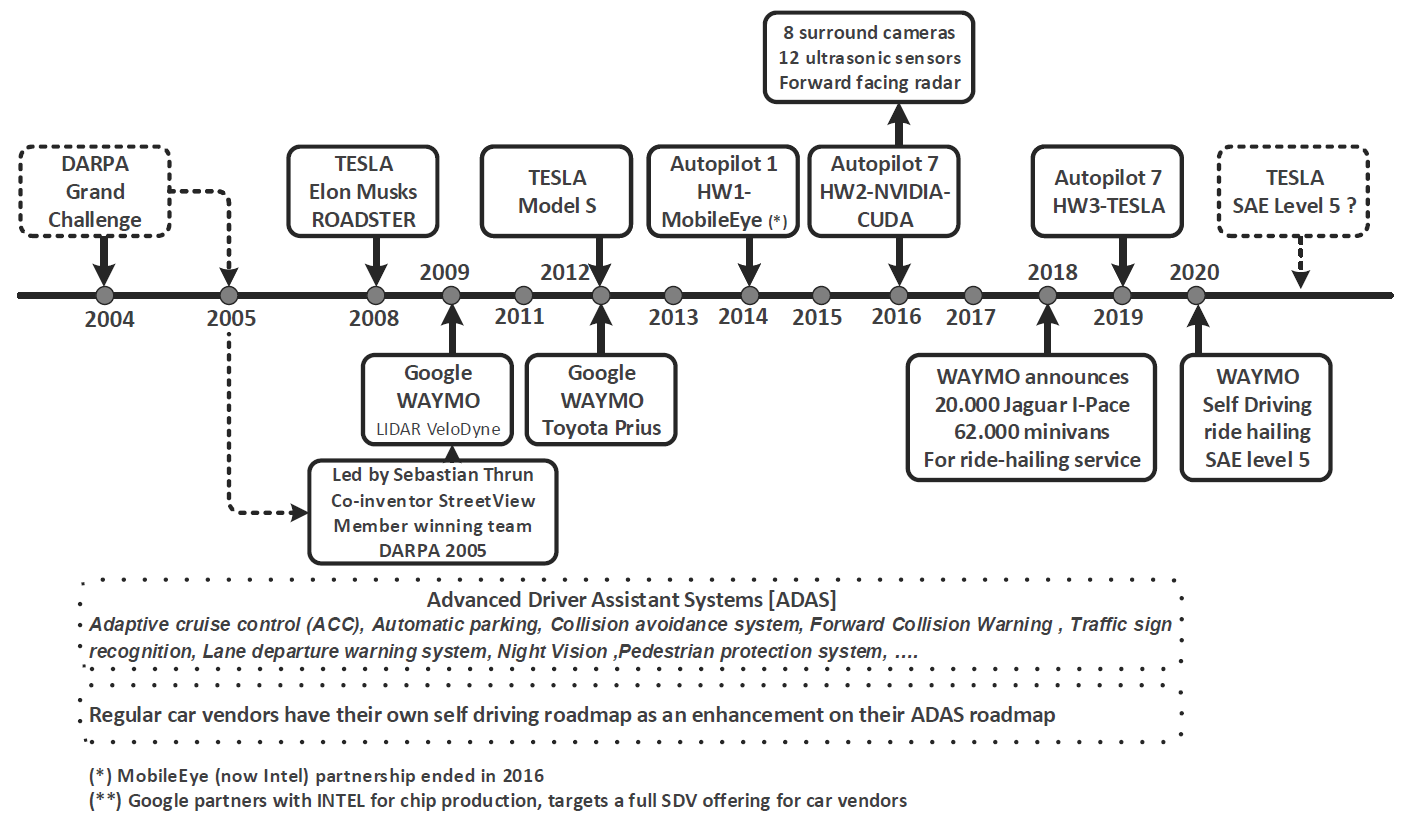
\includegraphics[width = \linewidth]{figure/SDV_evol.png}
\caption{Automated vehicle evolution}
\label{fig:AV_evol}
\end{figure}

Car drivers must continuously scrutinize the car surroundings as well as being able to quickly react. However, there is sufficient proof that a driver can be easily distracted by a conversation, tiredness, a phone call or even by looking at its vehicle system which compromises the driver awareness. Added to a constantly increasing road occupation, the potential risk of accident increases accordingly, requiring higher \acs{adas} performances. Thus, the next logical step of \acs{adas} evoltuion is to replace the human awareness by technical sensors, and, the human brain by a computer system which analyzes in real-time the captured data and reacts instead of the driver. Thoses decisions are next transformed into car actions using different actuators~\cite{DAS_handbook}. \acs{adas} is therefore evolving towards intelligent vehicle which instead of simply assisting the driver, it progressively replaces its intervention in driving situation; automated driving. 

As a result, vehicles have evolved from purely mechanical to electromechanical systems with increasing computerized control, making them more robot alike. When speaking of robots in the autonomous car context~\cite{Towards_Robotic_Cars} it is hard not to mention the \acf{darpa} of United States, leader of the \acs{darpa} Challenges. Those are meant to spur technology innovation through highly prized reward challenges which have been the spark to the research explosion about intelligent vehicles. Autonomous driving really took off with \acs{darpa} Grand Challenge in 2004 where the US military issued a challenge for any inventors to provide a car which could travel across the Majova Dessert. The first edition was far from successful as the best performer only drove driverless 12 km of the targeted 240 km route. Nevertheless, at the second edition of the challenge in 2005, five vehicles completed the full course autonomously. Less then two decades ahead of the DARPA challenge, \acs{adas} capabilities, autonomous research and prototyping has increased (as shown in~\textsc{figure}~\ref{fig:AV_evol}), and are no longer science fiction and will become a reality on next decades. 

		\section{Terminology and automation levels}
Many terminologies are used when arguing about intelligent vehicles, this section aim is to clarify the terms generally used, and to introduce the automation levels proposed by the \acf{sae} International~\cite{SAE}, the most quoted standard. The organism defined the way towards “automated driving under all roadway and environmental conditions” following 6 different levels; the higher is the \acs{sae} level, the more driving tasks are managed by the vehicle. 

\textit{Automated driving system}, according \acs{sae} terminology, is an umbrella term covering three automation stages~\cite{herrmann2018autonomous} from \textit{conditional automation} to the final \textit{full automation}. Autonomous vehicles, autonomous driving or self-driving vehicles, all refers to the highest \acs{sae} levels 4 and 5 whereas driverless cars refer only to the fifth automation stage. Those levels require a high intervention of machine solution, and are thus known as machine centered autonomy while level 1 to 3 are defined as semi-autonomous, or human centered autonomy since the driver is still leading. The actual people dream is vehicles of SAE level 5 capability where all aspects of driving control is handed over to the car system which is the actual target of the research field leaders. 

The SAE automation levels are illustrated in \textsc{figure}~\ref{fig:auto_levels} and described below:

\begin{figure}[hbtp]
\centering
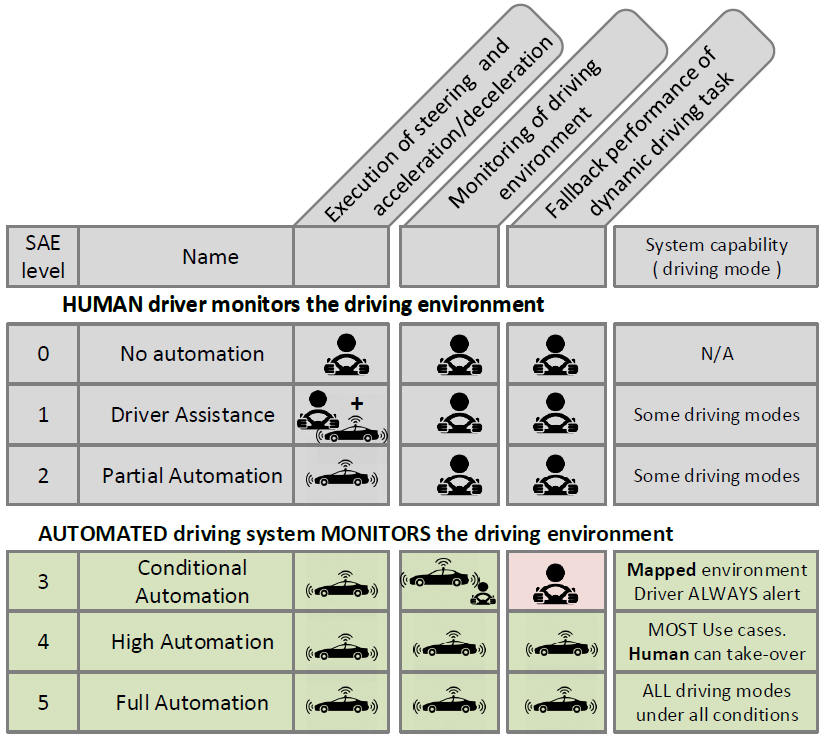
\includegraphics[scale = 0.6]{figure/SAE_levels.png}
\caption{SAE Automation levels (inspired from~\cite{SAE})}
\label{fig:auto_levels}
\end{figure}

\begin{itemize}
\item[(0)] Level 0 is the lowest level of automation which includes vehicles without any automated functions. The driver is entirely responsible of the actuation, and there is no intervention of embedded robotic systems.
\item[(1)] At level 1, the driver and the vehicle shares control for defined situations. For example, while using the parking assistance, the driver actuates the gas pedal while the vehicle steers the wheels. Another example is the cruise control, while the car is actuating the pedals, the driver controls the steering. Such level of automation requires the driver to perceive his environment properly, and to take over the control once requested. 
\item[(2)] At level 2, the driver can hand over the forward, backward and steering controls to the system for a certain amount of time or for a certain driving circumstances. Still, the driver must constantly monitor his environment and must be prepared to take over the control upon request. 
\item[(3)] From level 3, the driver is not compelled to permanently monitor the road and the vehicle indicators. Indeed, the system is capable of controlling the car autonomously in defined road contexts (driving modes). It also has the ability to determine its operational limits, and warns the driver to take the wheel back once the driving situation is out of bound. From level 3, the vehicle has a self-limit understanding; at this level, the vehicle is not capable of handling an out of bound situation. 
\item[(4)] Fourth level automated vehicles are capable to drive autonomously in some driving modes and no driver interaction is needed. The vehicle is capable to handle the driving from place A to place B in most situation. However, once the vehicle observes its own limit, the machine is capable to safely manage the situation (stopping appropriately for example), even if the chauffeur does not respond to the intervention request
\item[(5)] Level 5 is the fully autonomous or driverless vehicle; besides providing its destination to its transport, the human has no other involvement in driving, nor can intervene; at such of automation the vehicle has no longer attributes as steering wheels, or pedals and remains only a Human Machine Interface. 
\end{itemize}

Many car manufactures have taken part into the \acs{av} race because of the expected economic spin-off. \textsc{Figure}~\ref{fig:Navigant} is the result of the Navigant multi-criteria analysis survey which shows the leader-board of the main competitors. \textsc{Figure}~\ref{fig:MileDriven} presents the disengagement frequency relatively the mileage driven by prototypes on public road (according to their official reports).

\begin{figure}[hbtp]
\centering
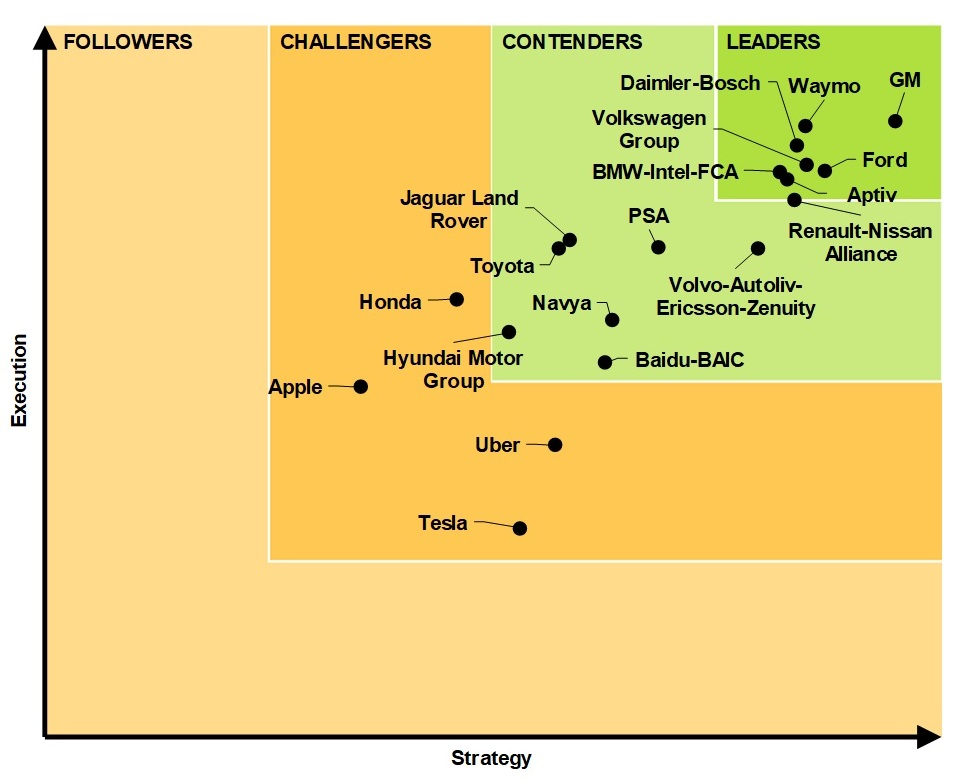
\includegraphics[scale=0.45]{figure/Navigant_leaderbord.jpg}
\caption{Main competitors in the autnomous vehicle race (2018)~\cite{Navigant_2017}\cite{Navigant_2018}}
\label{fig:Navigant}
\end{figure}

\begin{figure}[hbtp]
\centering
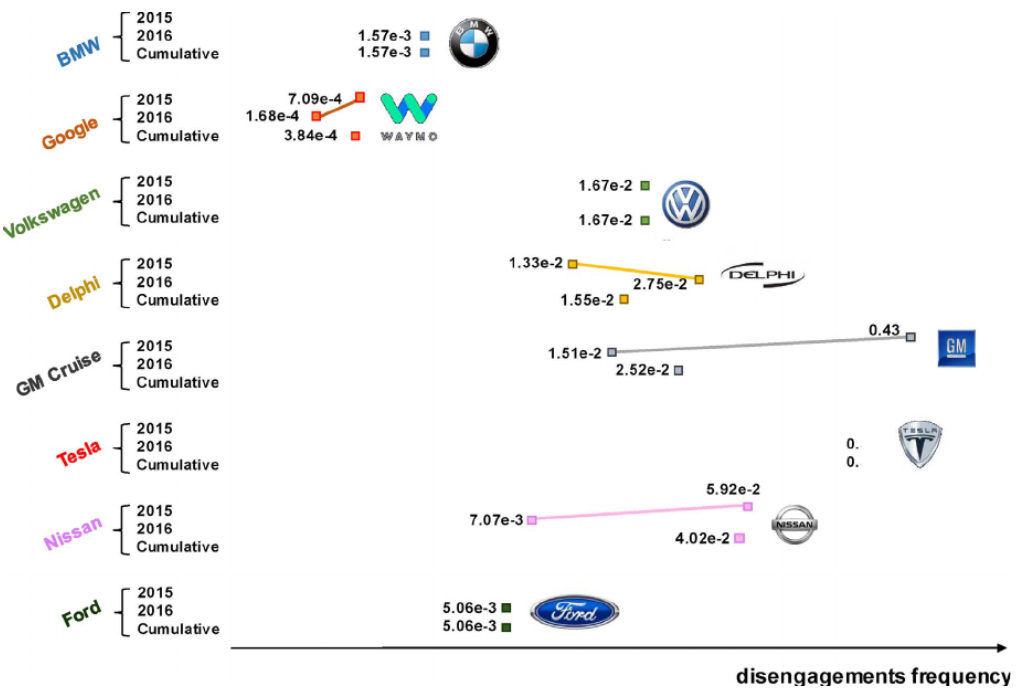
\includegraphics[scale=0.6]{figure/Disengement_freq.png}
\caption{Main auntonomous vehicle competitors disengagements frequency~\cite{FAVARO2018136}}
\label{fig:MileDriven}
\end{figure}


\section{Benefits and disruptions of driverless rides}
Self-Driving Vehicles may represent a huge, yet beneficial, disruption to the transportation sector. The benefits on safety, congestion and transport behaviour are promising~\cite{PrepaNation4AV}~\cite{AV_prediction_}.

The safety impact has already started with the democratization of ADAS components in cars. The introduction of Automated Braking Systems [ABS], detection and enforcing the safety belt, distance control has certainly reduced car casualties. Further reducing the human limitations will certainly contribute to increase safety.

Traffic jams can often be linked to inefficient driving and reducing commuting traffic time will be a social benefit.  Hundreds of working or leisure hours are lost on the roads. Intelligent drive would not only reduce commuting time but allow the passengers to do more useful tasks like placing phone calls, performing a video conference, reading the newspaper or just rest before arriving at the next meeting. And drivers would no longer need to chase for a free parking place as the car would be able to take care of it. 	

Transport behaviour would be impacted by the change of individual car ownership towards a car sharing model. Something like the Uber car sharing model but without need for drivers. 

But the introduction of self-driving car related technology would also impact many other aspects of the vehicle business. 

The impact on the electrical grid networks would be tremendous but would also introduce additional innovation requirements in battery charging. 

With the ability of vehicles to communicate with its environment via V2X (Vehicle to Everything) and its ability to have an in-depth analysis of its environment, why should there still be traffic lights on the roads?  Why should cars even continue to have headlights when infrared cameras are doing a better work in all lighting conditions. As with sound, light would be added to cars just to warn pedestrians or cyclists. SDVs will perhaps lead to less traffic jam on the existing infrastructures but will allow to rethink the infrastructure design for a more optimal utilization.

Computerized self-driving will improve road security by preventing accidents due to human errors but it could introduce severe insecurity due to computing errors. Such errors might only be caused by human coding mistakes but also to hacking. As with computer systems, hacking car systems will become a challenge for geeks but would also impact national security. 

Moreover, players like Waymo and Uber are clearly putting the taxi and truck driver jobs at risk. Perhaps the next generation will look at a taxi driver job like we currently look at a switchboard operator job in the telephony space. Considering the scenario where new software players like Google, Amazon, Uber get into the transport world with self-driving trucks. They would go into competition with players which need to struggle with human legacy like pensions and strikes due to extensive working agreements. A automated ride service company would have a strong asset over the existing companies. 

The supply chain optimization will be further automated and optimized. Self-driving trucks driven by software algorithms could led to better use of the transport capacity via automated optimal route and optimal store capacity calculation. This could be the "Just In Time" delivery without the current car jam problems which enforce delivery hours outside peak hours.

Consider no need for gasoline transportation and car parts which become obsolete (steering wheels, headlights, parts linked to combustion motors replaced by electric motors, etc.).

And not only charging pods are a prerequisite for the success of self-driving vehicles, an updated regulation and legislation is certainly required.  Less privacy due to internal cameras and usage logs. Accident problems will become lawsuits between service provider companies and not between individuals.

Lastly, until now car manufacturers are known for their “mechanical brand" and their challenge will be to introduce software technology into their systems without losing their brand name attraction. People start desiring the "TESLA brand" not because of their mechanical superiority but because of a "trendy desire". Their fear is that we would buy a "Waymo car" build by car brand x rather a car brand xx with software from Waymo (could compare it with the "Android phones").  

	\section{Autonomous vehicle system}
A vehicle is a mean to achieve a travel purpose; when the driver takes the steering wheel it is mostly with the willingness to go from a location A to a location B. Having this in mind, the driver knows which path to take to get at location B, using a mental map, GPS, road indications, etc.. Once the driver is on his way, he is constantly monitoring the environment and reacts accordingly to achieve his purpose safely. The human mechanism of driving is not different of what an automated car should manage, actually the computer must replace the human ability to drive in more or less situations depending on the level of automation. The driver may not realize how many difficult and  different tasks he is simultaneously accomplishing, but they are difficult to mimic by a computer.  

Due to their similitude, understanding how a lambda chauffeur drives is a strong start to understand automated vehicles framework. While on the road, human drivers need to answer four questions. The questions are listed below and a computerized illustration of how Waymo assesses the task is given in \textsc{figure}~\ref{fig:modeling}.  

\begin{enumerate}
	\item Where am I? (\textsc{Figure}~\ref{fig:WhatSurMe}) While traveling from A to B following a path, the driver can locate himself in the world and judge if he is on the right path. Moreover, he estimates the vehicle relative position on the road, thus he can drive on the correct area. The scientific field in charge of answering the positional question for automated vehicle is often referred to as \textit{localization and mapping}. 
	\item What is around me? (\textsc{Figure}~\ref{fig:WhereAmI}) The driver is able the recognize the objects such as pedestrians, vehicles, traffic signs or traffic lights, and so on around the vehicle. He is constantly aware of his surrounding and is able to read the signs or estimate the road participants' speed (for example). This tasks is known as \textit{environment perception and modeling}. The term perceiving stands for the ability to see, locate, understand, estimate pose, etc. of the road objects, whereas the modeling characterizes the way an automated vehicle makes an instant computer-intelligible model of the real world. Moreover, the perceiving task is also known as \textit{computer vision} in the other scientific field. 
	\item What will happen next? (\textsc{Figure}~\ref{fig:WhatWillHap}) The driver is skilled to anticipate the movements or the reactions of the other road participants. He instinctively knows the higher probability of pedestrian to cross a road when he is near a marked crosswalk, or the one of a car to turn right when its turn signal is switched on. This question is also addressed in the \textit{environment perception and modeling} task. 
	\item What should I do? (\textsc{Figure}~\ref{fig:WhatShouldDO}) Once the chauffeur has made a proper understanding of the surrounding, he decides what actions needs to be taken. He decides whether to continue, stop, slow down, park, leave the priority, etc. according to its journey purpose, the road laws or moral aspects, and so on. This task is named \textit{decision making and path planning}. After making decisions, the driver chooses the local trajectory and speed profile which he follows by actuating the gas/brake and steering wheel; in other word he manually control his car. For the automated vehicle, the \textit{decision making and path planning} provides an ideal path reference and a speed profile the car must follow. Afterwards, the \textit{motion control} automatically adjusts the commands to follow those references. 
\end{enumerate}
\begin{figure}[hbtp]
    \centering
    \begin{subfigure}[b]{0.6\textwidth}
        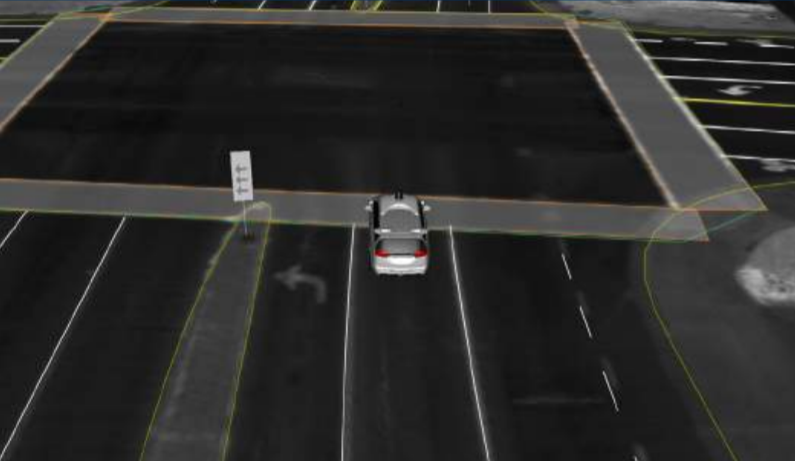
\includegraphics[scale=0.47]{figure/WhatSurMe.png} 
        \caption{Where Am I?}
        \label{fig:WhatSurMe}
    \end{subfigure}
    \hfill
    \begin{subfigure}[b]{0.6\textwidth}
        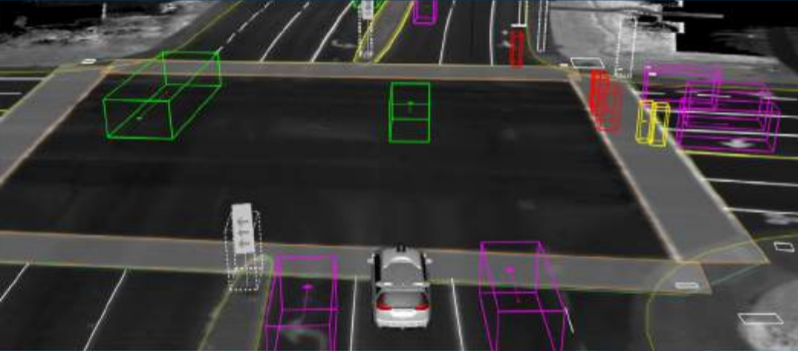
\includegraphics[scale=0.47]{figure/WhereAmI.png} 
        \caption{What surrounds me?}
        \label{fig:WhereAmI}
    \end{subfigure}
    \begin{subfigure}[b]{0.6\textwidth}
        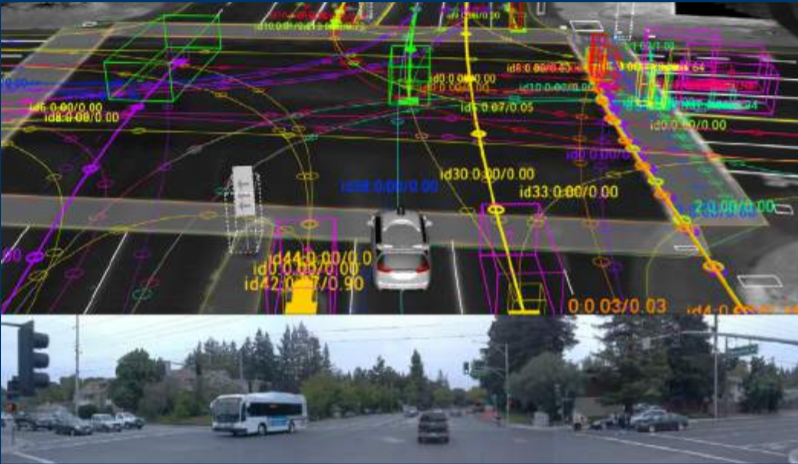
\includegraphics[scale=0.47]{figure/WhatWillHap.png} 
        \caption{What will happen next?}
        \label{fig:WhatWillHap}
    \end{subfigure}
    \begin{subfigure}[b]{0.6\textwidth}
        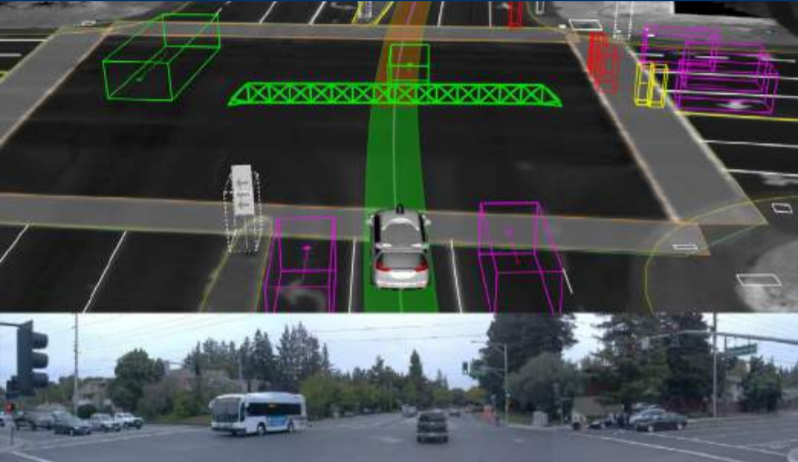
\includegraphics[scale=0.47]{figure/WhatShouldDO.png} 
        \caption{What should Ido?}
        \label{fig:WhatShouldDO}
    \end{subfigure}
    \caption{Google Waymo's framework process illustration~\cite{waymo_safety_report}}
    \label{fig:modeling}
\end{figure}

All four tasks given above interact with each other in sequential manner. It is necessary for the vehicle to know its location and its surrounding before making decision. Hence, it first builds a model of the environment accordingly to its location. Later, the model is provided to the decision module which compiles the final destination purpose and the environment statement to build a local path. Then, the motion control unit is in charge to follow the received trajectory. Finally, this sequence is repeated again and again in real-time to ensure the autonomous driving. 

\clearpage
\subsection{Autonomous vehicle framework}

One of the major outcomes of the \acs{darpa} Challenge is their software architecture used to automate the driving task, and the challengers' approaches have been adopted within many self-driving vehicle project~\cite{Towards_Robotic_Cars}. The principle is to divide the complex task into multiple and simpler functions~\cite{Hong_Cheng} which are based on the four human driving tasks presented above. Nowadays general \acs{av} framework divides the autonomous driving into multiple achievements detailed in \textsc{figure}~\ref{fig:basic_framwork} and enumerated below: 
\begin{itemize}
\item[--]  First \textit{sensing} replaces the senses of the driver by automotive sensors collecting internal and surrounding data which are provided later to the \acs{av} computer unit(s). 
\item[--] The \textit{processing unit(s)} treats the measured data (basically a tremendous amount of numbers) to extracts meaningful features from the environment such as detecting, classifying, tracking road objects and participants, anticipating their movements or locating the vehicle itself in surrounding. The processing unit(s) receives the sensors data and applies the \textit{computer vision} algorithms which outputs multiple road features and predictions. The units also use the sensors measurements the \textit{localize} the vehicle within its surrounding. 
\item[--] Then each extracted features and the vehicle location are fused together within a computerized \textit{environment model} of the real world in a process named \textit{perception and model}; it consolidates the measurements and the processing unit(s) interpretations results.
\item[--] Planning is the brain of the \acs{av}, it uses the environment model to make the right decisions which are translated into a vehicle language: a trajectory which guarantees to safely achieve the driving purpose. This trajectory is often divided into a lateral motion (the path) and a longitudinal motion (the speed).  This stage is crucial, and besides solving numerical problems, it also deals with moral issues. 
\item[--] The actuation part is in charge of providing the appropriate signals to the \acsp{ecu} in order to follow the trajectory; this is where the \textit{motion control} of the vehicle is ensured. 
\end{itemize}

Among a multitude of challenges, the main technical difficulty for achieving autonomous driving is developing its hardware and software. Indeed, \acsp{av} make use of complex algorithms processing huge amount of data from the sensors, in real-time. Thus, besides requiring a gigantic computational power, the processing unit(s) size must be reduced to be embedded as well as their power consumption. Moreover, the prototyping investment is enormous because it uses high-end technologies and sensors which are expensive; a vehicle cost which must be reduced in the future to target the global market. Additionally, the reliability of such intelligent system is questioned for their cybersecurity. Thus, \acsp{av} are undeniably a wealthy subject of interest, research and investment, but it still implies many challenges which needs to be solved. 

\acsp{av} are complex by nature and involve many different skills and technical knowledge inherited from software (computer vision, sensor fusion, artificial intelligence, etc.), hardware, security, control, communication, actuation, signal, mechanic, traction etc. It would be out of scope to develop the state of the art of autonomous vehicle in this master thesis. However, for this case study, a small overview of the sensors are presented below and specific literature is provided later to the reader willing to delve the topics.


\begin{sidewaysfigure}
\centering
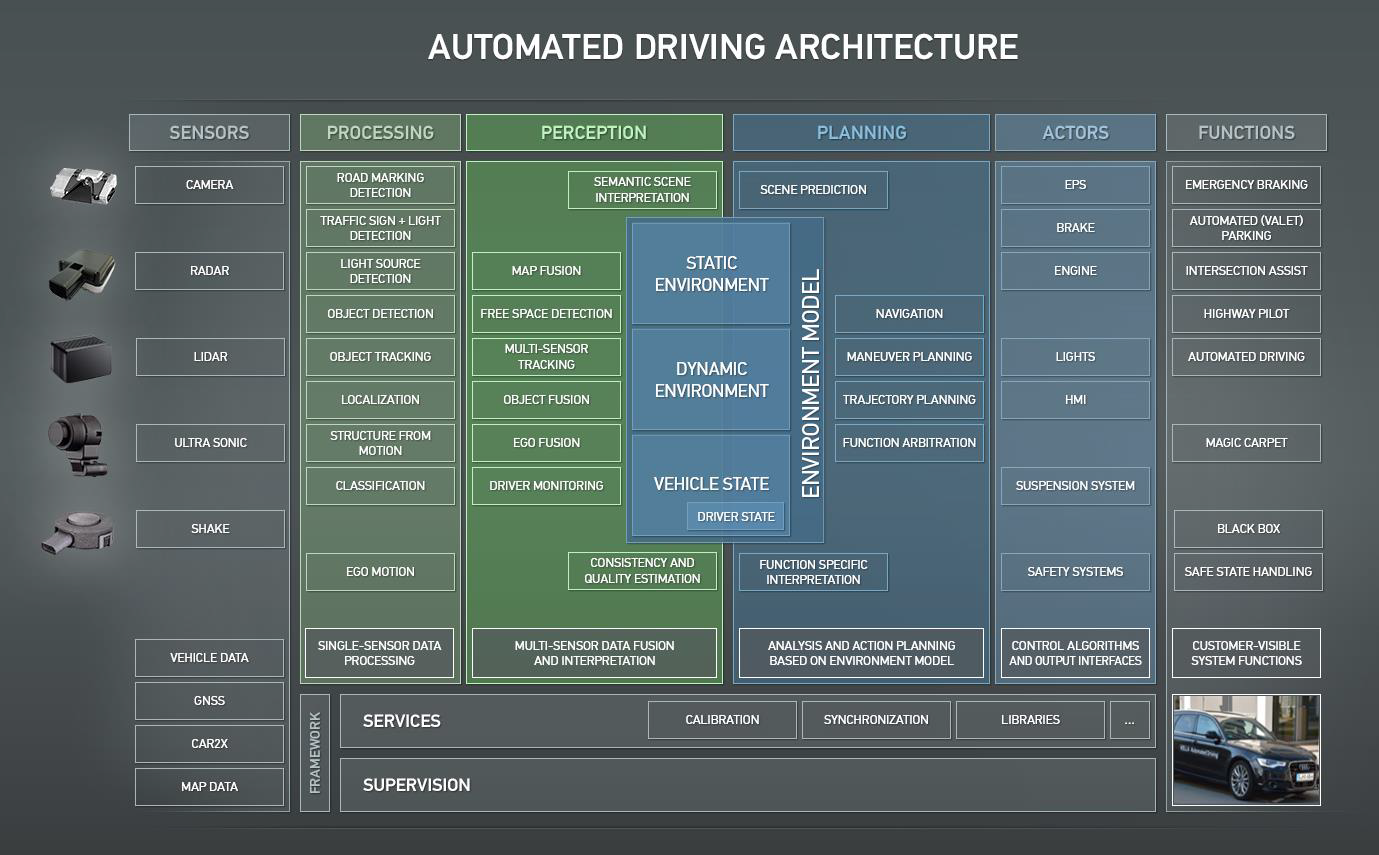
\includegraphics[width=\linewidth]{figure/SDV_detailled_framework.png}
\caption{Autonomous vehicle framework~\cite{Hella_slides}}
\label{fig:basic_framwork}
\end{sidewaysfigure}

	\subsection{Sensors} 
The human chauffeur relies on his senses and his perceiving ability to drive. As the human driver is about to be progressively replaced by autonomous systems, those capabilities must be replaced by a combination of hardware and software; this is partly the role of vehicle sensors and their associated processing units. Sensors are devices that are measuring physical quantities which are converted into a readable output signal, later transmitted to other devices. Sensors are already used in many field included automotive sector and their usage increased while \acs{adas} importance was rising. 

Autonomous vehicles inherit from the robotic field including the sensors terminology; sensors used to measure internal state are called \textit{proprioceptive} whereas devices used to measure external or surrounding environment are characterized  as \textit{exteroceptive}. 

Both type of sensors are used in the automotive sector; all proprioceptive sensors equipping a vehicle provides information about the vehicle state itself, which is also known as the \textit{ego-vehicle} concept. As a driver is capable to know the state of its transport mean, the automated vehicle must also be able to recognize system failures.

Environment perception is in charge of building a model of the surrounding using sensed data and specialized algorithms. Hence, it relies on computer-vision algorithms which extracts information from various type of data provided by exteroceptive sensors. In the automotive sector, thanks to \acs{adas} development, some sensors has shown to perform efficiently for automated driving. The most used are Cameras, \acf{radar}, \acf{us}, and lately, \acf{lidar} sensors. \textsc{Figure}~\ref{fig:archi} illustrates a typical usage and architecture of those sensors in a high-level-\acs{adas} vehicle. 

\begin{figure}[hbtp]
\centering
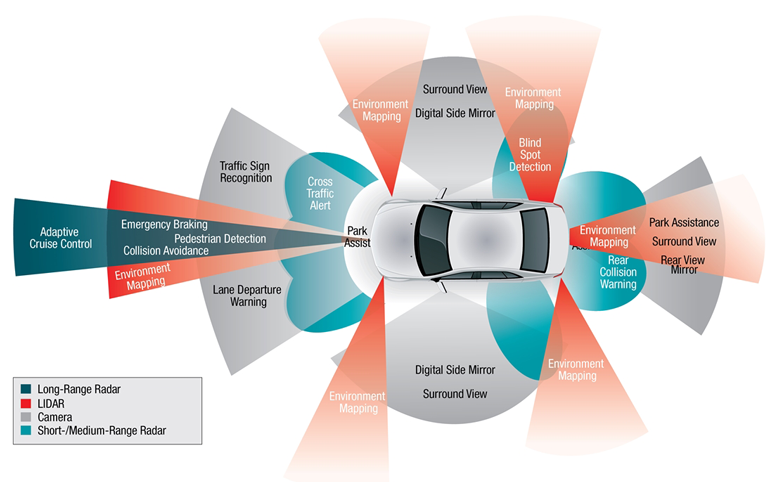
\includegraphics[width=\linewidth]{figure/SelfDriveCarSensors_Fig.png}
\caption{Autonomous vehicle typical sensor architecture~\cite{wendt_2018}}
\label{fig:archi}
\end{figure}

Cameras use visible light to build an image of the surrounding. They are the only sensor capable to capture color, contrast and texture within the same data output. Those information are tremendous for efficient computer vision algorithms. Moreover, those technologies are getting cheaper. Their drawback is the computation cost of the algorithms; due to the high number of pixel to evaluate, the computation time may be too long for automated driving need. Plus, they are sensible to light variation and does not work at all in dark conditions. Even if single cameras are not efficient at measuring speed and distance, by using two cameras working together (in a stereo fashion), it is possible to estimate those proprieties, but at high computation cost.

\begin{figure}[H]
\centering
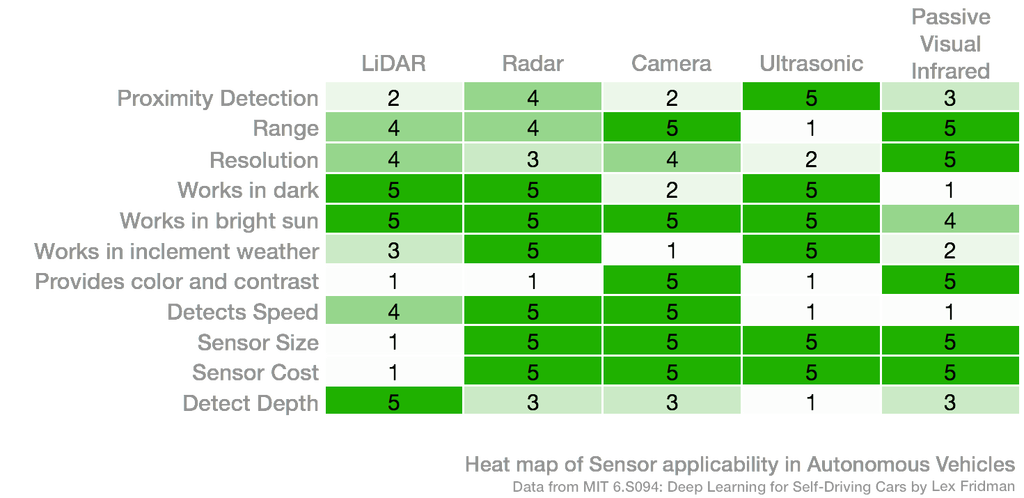
\includegraphics[scale=0.42]{figure/comparision_AV_sensors.png}
\caption{Automated vehicle sensor comparison~\cite{fridman_2}}
\label{fig:AV_sens_comparison}
\end{figure}

\acs{radar} uses reflected radio waves from the surrounding to sense objects. The technology is well known for aircraft or ship detection and have been miniaturized for automotive need. The technology is cheap and able to directly measure distance and estimate speed using Doppler effect, involving small computation performance requirements. They insensitive to weather and light changes, dust, rain or fog that could occur in driving condition.  However, the measure is generally noisy and the lack of contrast and color makes other information than distance and speed difficult to obtain. Plus, they perform better when sensing metallic objects such as vehicles but suffer when detecting pedestrian and plastic objects. 

\acs{lidar} sensors scan the environment with a non-visible laser beams. The beams makes it possible to visualize objects and measure ranges to create a 3D point clouds of the car surrounding. Its major disadvantages is that they are expensive (currently around 70.000\$) and they are not yet miniaturized. Their precise depth measure and high resolution provide a depth 3D maps of the surrounding appreciable in the perceiving and localization phase.

A comparison of the four sensors is provided in \textsc{figure}~\ref{fig:AV_sens_comparison} and highlights each sensor advantages and drawbacks. For achieving the environment perception and localization in every weather and lighting condition, there is no perfect sensor, and therefore it highlights the necessity of achieving the sensor fusion. 
	\section{Summary}
The levels of automation proposed by the \acf{sae} were introduced where fully automated cars (or autonomous vehicles) are characterized by the highest levels 4 and 5 of automation.  “Automated vehicle technology” is presented by the media and understood by the public as brand new while we have been surrounded by various types of automated vehicle systems for decades. What is new is the automation level that will allow full autonomous driving, eliminating the human actions not only for "acting" the system but also for "brain control".

The \acs{darpa} Challenge was the historical shift when intelligent vehicles had grown from research into a real industrial interest, with major investments from companies. In less than two decades we went from the first (non-working) prototypes to announcements of commercial self-driving cars. 

Highly automated vehicles are complex to achieve. Cars are no longer a purely mechanical business but require multiple expertise domains including more and more Information Technology (IT hardware and software). Automated and autonomous driving are achieved using a divide and conquer methodology, where complex tasks have been subdivided based on the real human driver behavior. The four main domains are environment perception and modelling, localization and mapping, decision making and motion control. Replacing the "human brain" control introduces the need for performant analysis of the surroundings by sensors.

Proprioceptive sensors are mainly used to build ego-vehicle knowledge, whereas exteroceptive sensors are used to achieve environment perception, localization and mapping. From the wealth of sensors available on the market, four types have shown to be useful in driving automation namely LIDAR, cameras, RADAR and ultrasonic sensors.
	
Sensors are certainly not new in car automation field. The sensing challenge of autonomous vehicle is to implement the \textit{sensor fusion} using a highly powerful computer unit. A power unit capable of using all the collected data to recognize individual objects like pedestrians, traffic signs and lanes (\textit{perceiving}), to detect where he is exactly positioned in that surrounding (\textit{localization and mapping}) but also to autonomously decide the appropriate actions to safely travel through that environment (\textit{planning}). Next, using the planned trajectory, the vehicle applies\textit{ motion control} techniques to follow the trajectory. 

The autonomous vehicle is a large field of research and development that requires different technical skills like mechanical, hardware, software, signal, safety, control engineering and so on. From the presented framework of \acs{av} and my own skills in control, it has been decided to focus this master thesis on the \textit{motion contol}. 
	

\section*{References}

This section proposes some references I have found useful for growing a general knowledge on autonomous vehicles. A literature review has already been proposed in~\cite{rosenzweig_bartl}; the author highlights the increasing number of publications directly related to the increasing interest and investments over the years. The author summarizes many publications related to the autonomous vehicle field, hence this document might be used as a database when starting a topic investigation. 

With the growing popularity of \acsp{av}, some interesting books have recently been published. \cite{McGrath_AVOSD} is an entry level book about self driving vehicles; the author offers a primer for readers who are unfamiliar with this industry.~\cite{roland_berger} is a straightforward introductory document about self driving cars. \cite{herrmann2018autonomous} develops further the topics covered in the previous documents; from \acs{av} technology, mobility trends, economic and society impacts, issues to be addressed, this book covers many subjects on autonomous vehicle and provides an elaborated bibliography. \cite{MIT_Driverless} is a book proposed by the MIT, and covers the same aspects than the previous one. \cite{liu2017creating} is a collection of the authors' publications that covers the entire technical aspects of autonomous driving; they introduce the challenges and the techniques, then describe their poposed solutions. Technically speaking, \acsp{av} inherit many concepts from the intelligent robots which are described in \cite{Siegwart}. A survey about the computer vision method applied to autonomous vehicles has been proposed in~\cite{Computer_VisionForAV}; althought it is very throrought, it requires a basic knowledge of machine learning. Both \cite{MotionPlanSurvey} \cite{Modeling_Control_Strat} propose a survey on motion planning, longitudinal and lateral control of \acs{av}. The MIT proposes a free online lecture about deep learning for self-driving cars ~\cite{fridman_2} while Udacity proposes a complete (charged) course about \acs{av}~\cite{Udacity}. 

%\begin{figure}[hbtp]
%\centering
%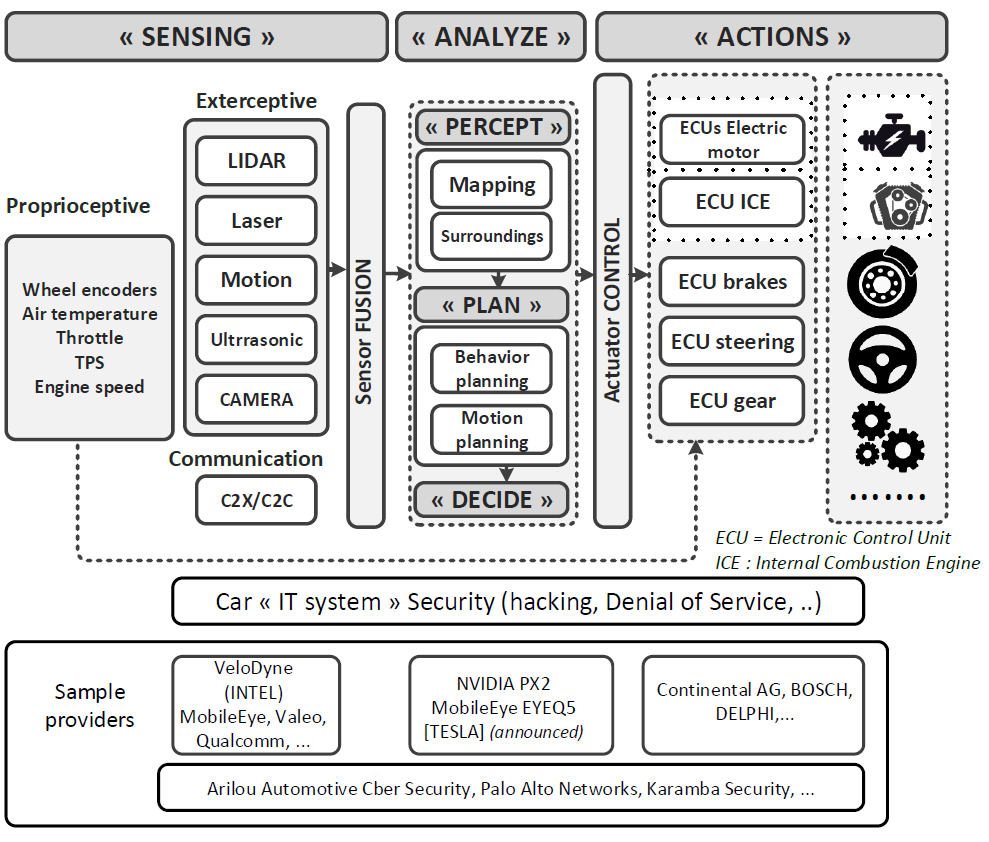
\includegraphics[width=\linewidth]{figure/SDV_framework.png}
%\caption{Autonomous vehicle framework (inspired from~\cite{Hong_Cheng})}
%\label{fig:tepmp}
%\end{figure}


\chapter{REVAi electric vehicle presentation and diagnostic \label{chap:reva}}
The \acf{vub} is willing to investigate the automated vehicle field, and moreover, they want to prototype such a vehicle. The \acs{vub} owns an electric car which is intended to be used as a development platform for experimenting  automated features. However, the platform was previously damaged and not operational at the beginning of this master thesis. As I was willing to practically develop an automated feature, I needed to fix the development platform. 

This chapter explains the general working principle of electric vehicles and presents the prototyping platform. After proposing and implementing a solution to solve the vehicle problem, different analyses and measurements were conducted to verify its working state. Some results are presented in this chapter, and a conclusion of the prototype state is proposed. 

	\section{Electric vehicle}
Nowadays vehicles can be classified in 3 categories depending on the type of embedded motor/engine used. Most common vehicles are employing \acf{ice} while \acfp{ev} uses electric motors. \acfp{hev} use both technologies. As this chapter is dedicated on the \acs{vub}'s prototyping platform which is an electric vehicle, only \acs{ev} will be introduced. 

\acsp{ev} use electrical motors for producing the traction effort and chemical batteries, fuel cells or capacitors as its rechargeable energy source. Such vehicles posses advantages over \acs{ice} vehicles making them a good alternative choice. \acsp{ev} perform with an efficiency above 90\% in certain operating regions while an \acs{ice} is limited to 40\% at best. Additionally to the high efficiency, EVs produce zero local emissions, low power consumption and enable independence of petrol market. Nevertheless, \acsp{ev}' drawbacks are their higher initial cost, limited driving range, limited battery lifetime, and their long charging time. Those are important disadvantages which needs to be solved in order to make \acsp{ev} competitive on the vehicle market currently dominated by \acs{ice} vehicles. By using both techonolgies \acsp{hev} try to combine the advantages of electric vehicles and internal combustion engines by providing higher efficiency and longer driving range. \cite{HVT,ModernEV} 

\begin{figure}[hbtp]
\centering
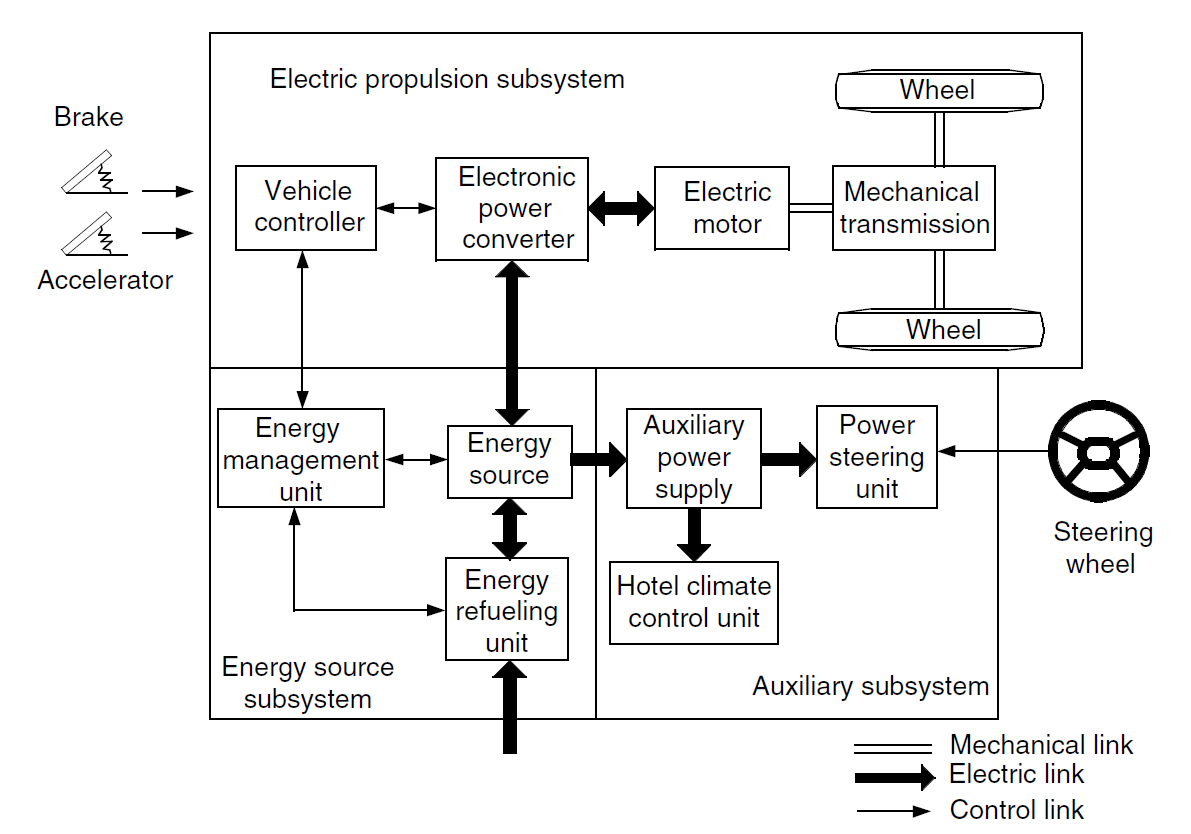
\includegraphics[scale=0.5]{figure/Conceptual-illustration-of-general-EV-configuration.png}
\caption{Conceptual illustration of general EV configuration~\cite{ModernEV}}
\label{fig:EVconceptual}
\end{figure}

The modern electric vehicle working principle is conceptually represented in \textsc{figure}~\ref{fig:EVconceptual}. As shown in this figure, thee major subsystems are embedded within \acsp{ev}: (1) the electric propulsion subsystem, (2) the energy source subsystem and (3) the auxiliary subsystem. Each subsystem is interacting with the others by transferring power trough electrical links, or information trough control links. 

The \textit{energy source} subsystem comprises the energy source itself (like batteries) which supplies the vehicle with electrical power, the refueling unit which enables recharging the energy source, and the \acf{ems}\footnote{or Energy Management Unit (EMU)} which monitors the electrical system state and the power flow. Using its measurements, the \acs{ems} regulates the energy flow and optimizes the energy usage. Therefore, the role of the device in \acs{ev} is crucial since its quality affects the vehicle autonomy and general behavior. 

The \textit{auxiliary subsystem} is in charge of supplying each auxiliary system such as the headlight, turn signals, the steering helping process, etc. 

Finally, the \textit{electric propulsion subsystem} is the main part of an electric vehicle. Given a throttle and a brake pedal input, the vehicle controller computes and provides the electronic power converter with the adequate control signals. The power converter regulates the energy flow from the batteries toward the motor by modulating an electric signal. Additionally, the energy management unit cooperates with the vehicle controller to ensure correct energy transmission with regard to the vehicle state and for safety matter. The energy flows are bidirectional since the electric vehicle can recharge its batteries in a regenerative process. As well, a communication is ensured between the energy refueling unit to ensure proper charging sequence.  

There is a variety of practical implementations of electric propulsion system. Early electric vehicles were a derivation of \acs{ice} vehicles where the engine was simply replaced by an electric motor and a battery pack while the gearbox and the clutch were kept. Nowadays electric vehicles are equipped with a motor drive that ensures the role of the clutch and the staged gearbox. Actually, the power/torque - speed characteristic of a controlled electric motor allows to remove the traditional gearbox of \acs{ice} vehicles, relieving some weight. \textsc{figure}~\ref{fig:EVpowertrain} represents a classical drive train topology currently used. The figure highlights the main components; the electric traction motor and its attached power converter (DC/DC, DC link and the inverter). Due to their importance, those components are detailed in the following subsections. However, the vehicle differential is still in use for \acs{ev}, even if some experimental designs propose removing them.  It is usual to find a single stage gearbox to reduce the high rotating speed of the motor going to the wheels. Removing those mechanical transmission allows reducing the weight, hence decreasing the necessary embedded the power storage or incresing the range. Therefore some research is done to remove the differential and the gearbox which implies to place a motor to each driving wheel~\cite{HVT,ModernEV} . 

\begin{figure}[!ht]
\centering
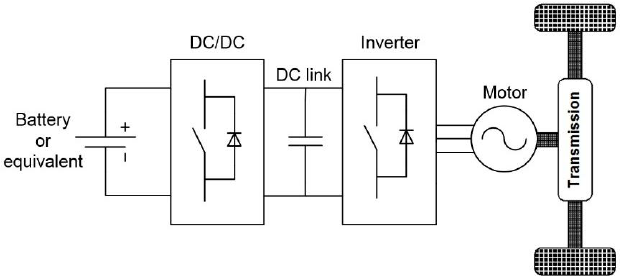
\includegraphics[scale=0.55]{figure/Powertrain-topology-of-a-battery-electric-vehicle-used-in-this-paper.png}
\caption{Drivetrain topology of a battery electric vehicle drivetain~\cite{en8020921}}
\label{fig:EVpowertrain}
\end{figure}

Electric vehicles and hybrid electric vehicles popularity is taking off and are part of the mobilty mega-trend like the vehicle automation~\cite{McGrath_AVOSD}. \acf{av} is technology based platform which is meant to compute electric signals while electric vehicles can be easily controlled by such signals. It appears that \acs{av} and \acs{ev} are more compatible than would be traditional \acs{av} and \acs{ice} vehicles, or at least, they present a better interoperability~\cite{McGrath_AVOSD}. 

		\subsection{Electric motor}

		An electrical machine is a general term for machines that uses electromagnetic forces to provide mechanical power from electricity and vice-versa. When such machines are converting electrical power into mechanical power, it operates as an electric motor, and, oppositely when the mechanical power is converted into electricity, the electrical machine operates as a generator. In general, motor and generator have the same build and are capable to work in either mode depending on the situation. The electrical machine is used in \acs{ev} as a motor producing the traction effort to overcome the resitive forces, and as a generator when producing electricity to recharge the batteries (in regenerative process).
		
Electrical machines have been massively used in the industry and appeared to replace efficiently \acs{ice} with the \acs{ev} market rise. The primary limiting factor was the short running distance which was restraining the usage of such motor. However, energy storage improvement has increased the possible range and made electric motor a suitable competitor to \acs{ice}. Additionally, those motors have a better efficiency, are smaller, lighter, fast torque responding and are easier to control compared to \acs{ice}~\cite{ElectricDriveEV}.

The first classification is made between \acf{dc} and \acf{ac} machines; a DC machine is using direct current (or voltage) while an AC machine utilizes alternative current (or voltage). Currently, brushed, brushless and permanent magnet brushless DC motors are used in vehicle traction as well as induction and switch reluctance AC motor~\cite{ElectricDriveEV}. Explaining all the different electric motor and highlighting each advantages and drawbacks is out of scope. Nevertheless \cite{SurveyMotor} provides a comparison of the different motors used in electric traction. However, since the prototyping platform of the VUB is using an induction motor, this particular one is presented below. 

The \acf{im}\footnote{or asynchronous motor} is an \acs{ac} electric machine used to produce mechanical power. Such motor comprises a stator and a rotor which both carry a 3-phase wiring. The \acs{im} exists in two fashions, the wound type motor have a short circuited 3-phase wounded rotor and the squirrel one is a simple metallic squirrel cage rotor short-circuited at its extremities. The squirrel cage motor is simpler to build and thus cheaper to manufacture. Each stator wiring is spatially placed at an equal angle from the two others and each stator phase terminal is connected to one of the 3 phase \acs{ac} power supply. Once an \acs{ac} current flows trough each phase, the spatial and temporal offset between each phase produce a rotating field, even if the stator remains fixed\footnote{thus the stator is called the inductor}. The rotational speed of this field is known as the synchronous speed and it varies with the supplied current frequency and the machine number of magnetic poles. Once the rotor is rotating below the synchronous speed, its conductors are perceiving a flux variation producing a potential difference across each rotor phase. Because the rotor is short-circuited, a current starts flowing through the conductor from the positive to the negative terminals. However, a conductor which has current flowing trough it in a variable rotating field sees a force applied to itself. Each rotor conductors is subject to this inducted potential difference and are then subject to an electromagnetic force. All those forces happen on each conductor placed on the rotating field which produce the torque at the rotor shaft; the motor torque. Once the rotor reaches the synchronous speed, its wires do not perceive a flux variation anymore, and thus the current stops flowing trough it as well as the induced torque vanishes. Oppositely, when the rotor slows down, the perceived flux variation increases, increasing the current and its associated force. Therefore, the rotor of the \acs{im} never reaches naturally the synchronous speed but will never be far from it; the difference between the rotor speed and its synchronous speed is known as the slip~\cite{wildi}. A typical mechanical characteristic (or its torque-speed curve) of an induction motor is presented in \textsc{figure}~\ref{fig:TorqueSpeedCurveIM}.

\begin{figure}[hbtp]
\centering
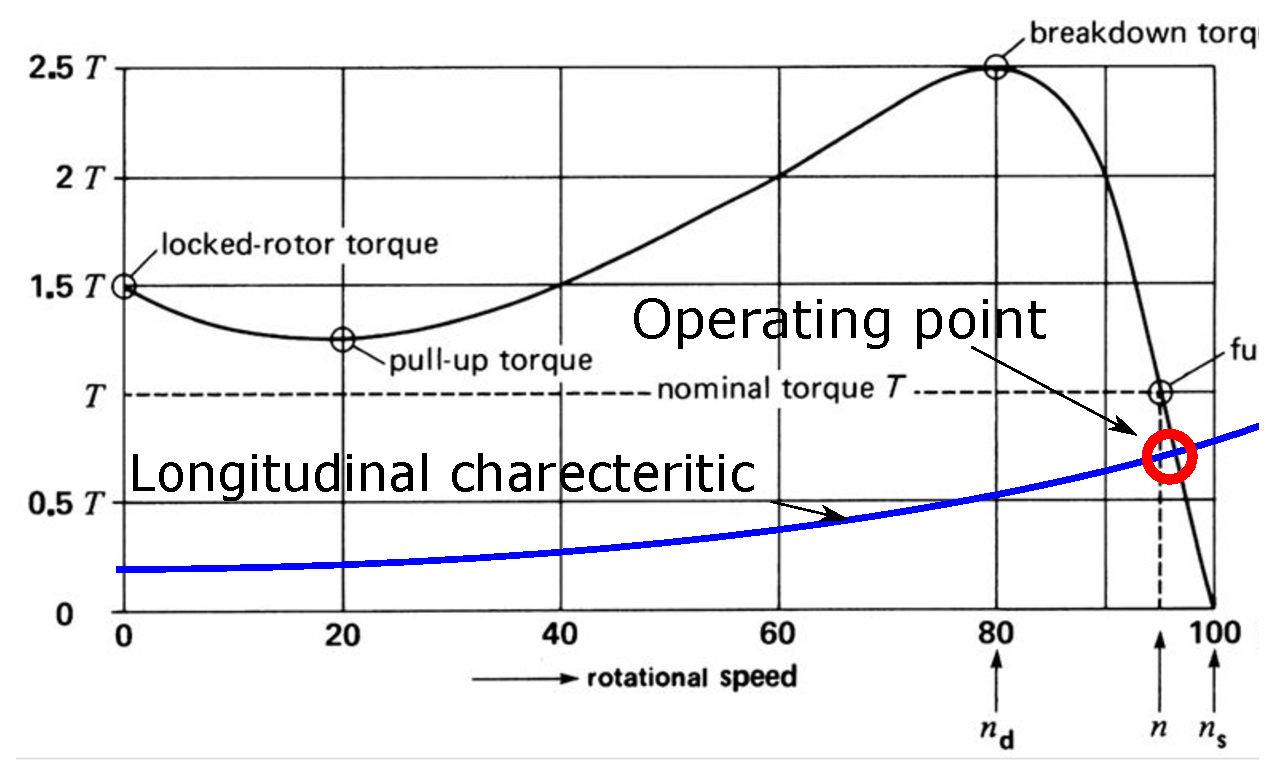
\includegraphics[scale=0.6]{figure/TC.eps}
\caption{\acf{im}and longitudinal characteristic(adapted from~\cite{wildi})}
\label{fig:TorqueSpeedCurveIM}
\end{figure}


	\subsection{Physical understanding of speed regulation}
When someone is driving on the road, the driver constantly pushes or releases the throttle. Indeed, external forces are applied to the vehicle and produce a resistive torque at its wheels. In order to stay in  motion the vehicle must produce a forward torque to compensate these external forces. 

This longitudinal dynamic is classified in two categories, (1) the power train and (2) the vehicle dynamic.  First, the power train dynamic comprises all the moving mechanical components which produces energy losses. Secondly, the vehicle dynamic illustrates all the external forces applied on the vehicle. It comprises the rolling resistance (or the friction between the road and the tire), the tire resistance caused by its deformation while rotating, the aerodynamic drag caused the air flowing around the vehicle and the gravitational forces. In \cite{rajamani2011vehicle} the longitudinal dynamic mathematical model is provided. As the induction motor, the longitudinal dyncamic is characterized by a torque - speed curve as illustrated in \textsc{figure}~\ref{fig:TorqueSpeedCurveIM}. The intersection between the \acs{im} and the longitudinal characteristic determines the vehicle speed. 

However, the desired speed and the external forces applied on the vehicle change constantly and therefore it is necessary to modulate the torque - curve characteristics to drive at any speed; this is the role of the motor drive. 

		\subsection{Motor drive}
Among multiple vector control methods for induction motor, the REVA uses an \acf{ifoc} algorithm (\textsc{figure}~\ref{fig:IFOC}). The idea of such a method is to apply the appropriate coordinate transformation to realize the torque and the flux control independently. In particular, the 3-phase (a,b,c) coordinate system is transformed into 2-phase ($\alpha\beta$) system, which is rotated by an angle $\theta$ to obtain a $dq$ coordinate system. The angle $\theta$ is chosen to align the flux with the $d$ coordinate simplifying the motor equations, and it estimated using the motor measurement $\omega$. Then, the torque can be controlled using stator current along $q$ axis ($i_{q}$) and the flux can be controlled using the current along $d$ axis ($i_{d}$). 

\begin{figure}[hbtp]
\centering
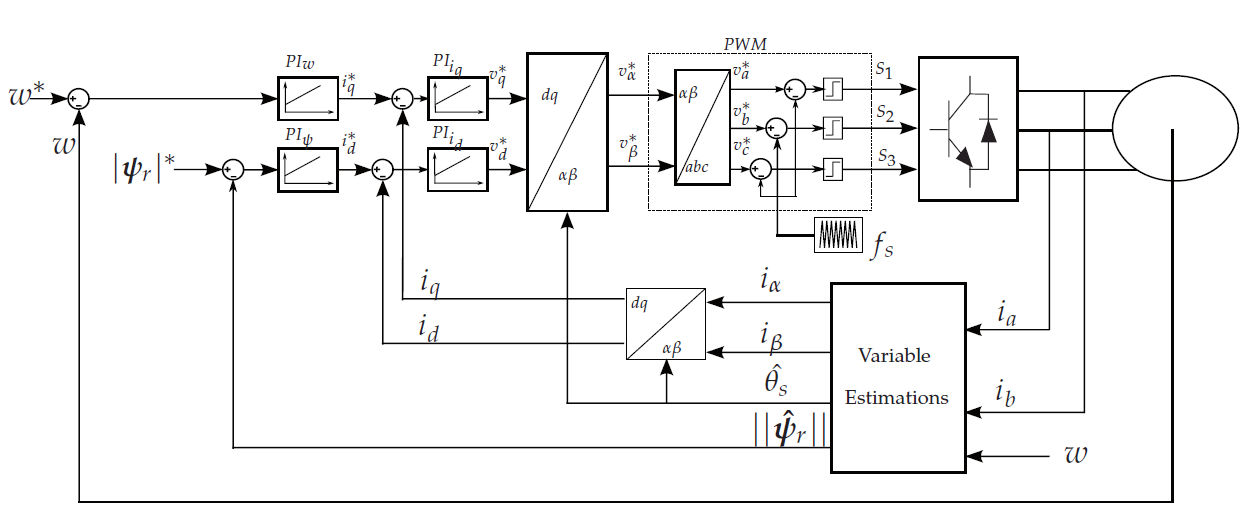
\includegraphics[scale=0.5]{figure/Block_FOC.png}
\caption{Block diagram \acs{ifoc}~\cite{en11010120}}
\label{fig:IFOC}
\end{figure}

Notice the unique motor feedback (\textsc{figure}~\ref{fig:IFOC}) is its rotational speed $\omega$ which estimates, using $i_a$ and $i_b$ respectively the stator current from phase a and b, the motor flux $\psi_r$ and torque (associated to the value $i_d$ and $i_q$). This characterizes the behavior of an \acs{ifoc} while a direct FOC, would use a direct measure of those values instead of estimating them. Indeed, placing the required sensors inside \acs{im} confined volume for such measurements is expensive, and thus \acs{ifoc} is most popular of the two solutions. In \textsc{figure}~\ref{fig:IFOC}, the \acs{ifoc} is configured in speed control mode and will follow the speed reference $\omega^*$. Such control algorithm is capable of working in torque control by directly regulating $i_q^*$. 

	\section{Description of REVA}
The REVA is an electric vehicle model manufactured by Mahindra Electric Mobility Limited located in Bangalore in India. The Company's goal is to develop and produce affordable electric vehicles. Four years after its creation in 1994, the first REVAi shown in \textsc{figure}~\ref{fig:REVAi} was launched. It was available in many countries such as France and Great Britain, however their success was not brilliant in European countries due to safety flaws and missed market strategy. Indeed, even if the price was attractive, the limited performance was refraining the potential buyers in Europe. 

The \acs{vub} acquired one of this electric vehicle in a none-operational state as a research platform for their students. Some of them proposed a general description of the vehicle and search the problem cause~\cite{REVA_anal}. This document provides a comprehensive survey of the REVA, and stated the vehicle problem was caused by a battery defect. 

\begin{figure}[hbtp]
\centering
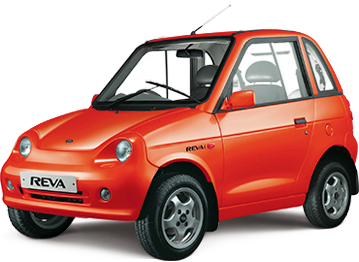
\includegraphics[scale=0.6]{figure/revai.png}
\caption{REVAi}
\label{fig:REVAi}
\end{figure}

REVAi is a rear wheel driven electric vehicle designed for city usage. The range could reach 120 km while driving at the maximum speed of 80 km/h. It weights 565~kg when empty and the vehicle brakes are using 4 mechanical drum brakes at each wheel. The vehicle is not steer-by-wire and the front wheels are steered using a mechanical shaft. 
 
\subsection{Topology}
A simplified wiring scheme is provided in \textsc{Figure}~\ref{fig:REVAi_topology}. As illustrated the car can be charged via \acf{dc} connection allowing fast-destructive charging and \acf{ac} plug allowing safe-slow charging. Neither of the cables is available in the lab, therefore, the battery pack had to be charged via another supply system. In order to charge the batteries from external power supplies, the car is equipped with a converter to modulate the electric power flow.

The unprovided internal power supply was 48 V - 200 Ah Li-Acid batteries. Originally the REVAi existed in other model using Li-ion batteries that increased durability and power density. 

Relays are used to control the different charging scheme. Those are regulated by the \acf{ems}. The relay SW 180 is switched ON and OFF by the contact key, thus it is the main relay of the vehicle. The scheme is similar to the one presented earlier in the chapter, with all parts working as a group. 
\begin{figure}[H]
\centering
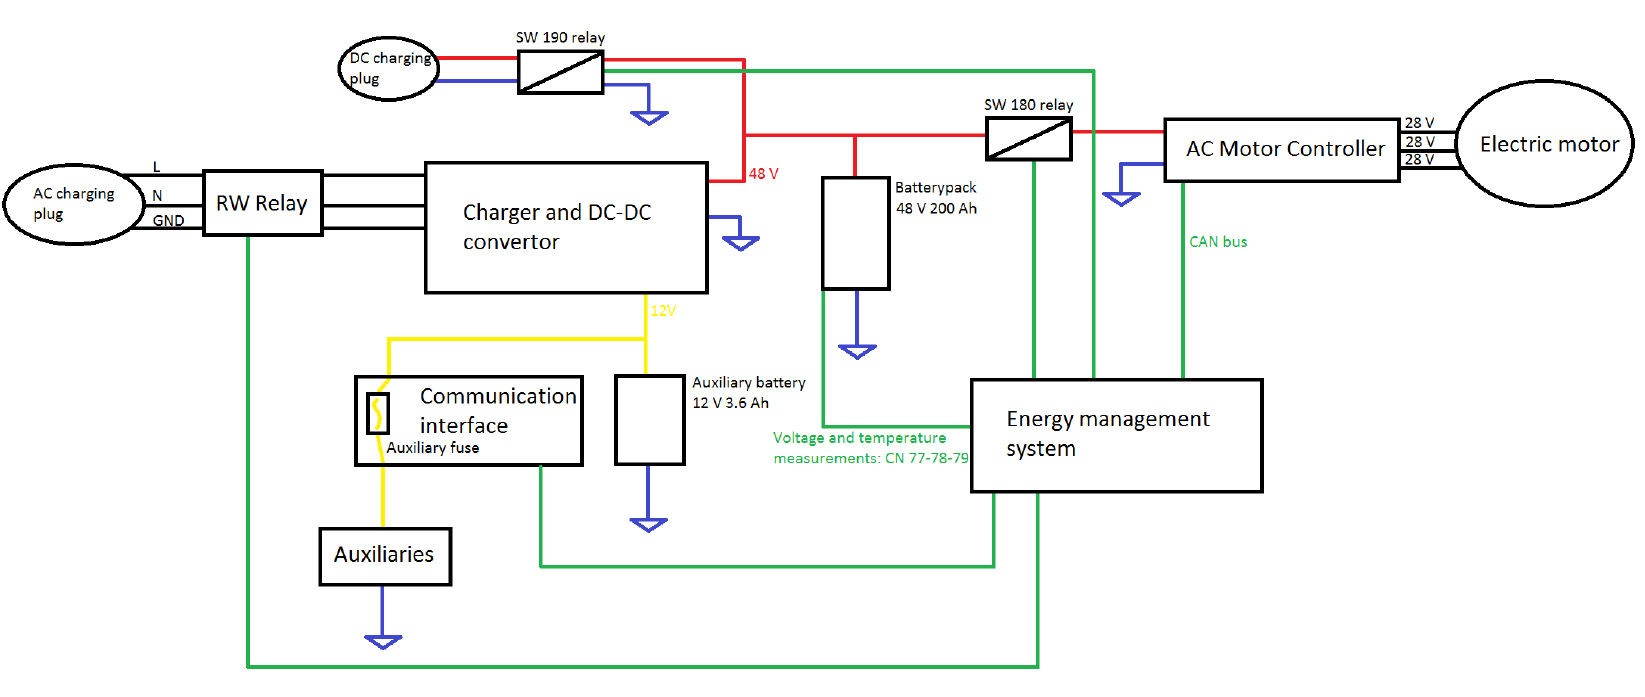
\includegraphics[width=\linewidth]{figure/REVA_topo.png}
\caption{REVAi Topology \cite{REVA_anal}}
\label{fig:REVAi_topology}
\end{figure}

\subsection{Energy management system and communication interface}
The REVA L-ion \acf{ems} monitors the batteries, measures the power consumption, and acts appropriately to maximize the driving range and ensure safety. There is no data-sheet currently available at the \acs{vub} for the \acs{ems}; however, the communication interface PCB shows that it is manufactured by Mistral Solutions Private Limited who is based in India. The manufacturers of the \acs{ems} itself is Incap Contract Manufacturing Private Limited, also located in India. Both of them could not provide their product data-sheet. 

The REVA communication interface linked to the \acs{ems} is located behind the front seat. It provides an access to the vehicle information via several ports: \acf{can} bus, RS 232 and USB. Accessing the REVA trough those port requires a dedicated Windows software named \textit{iEMS Analyzer} which is not freely available. Moreover, a password is required to access the software interface, password not available for external other then Mahindra. The \acs{can} port is physically accessible and it is possible to monitor the raw \acs{can} data-frames, but interpreting the information transferred via those frames is a complex task (car hacking). 

\subsection{Motor}
The 3-phase squirrel cage \acf{ac} is manufactured by Kirloskar Electric Company Limited in India. It is screwed at the vehicle chassis and its output shaft is directly connected to the rear wheels axle through a 9,4:1 signle staged gear box and a differential. It can provide a maximum power of 14.5~kW at 28~V and 3000~RPM. 

Those information are the only available from the manufacturer which was not disposed to provide additional information\footnote{Mahindra did not respond to my email}. Further research was not successful to find this induction motor data-sheet. 

\subsection{Motor controller and power converter}
The Curtis 1236 is an embedded \acs{ac} controller for induction motors manufactured by Curtis Instruments (United States) and designed for electric vehicle traction and hydraulic pump regulation. From the pedals actuated by the driver, the Curtis generates the appropriate \acs{ac} signal to control the induction motor. Therefore, referring to \textsc{figure}~\ref{fig:EVconceptual}, Curtis 1236 comprises the \textit{vehicle controller} and the \textit{electronic power converter}, making this device an important component within the REVA. 

\begin{table}[hbtp]
\newcolumntype{Y}{>{\centering\arraybackslash}X}
\begin{tabularx}{\textwidth}{ |Y|Y|Y|Y| }
\hline
\textbf{Model Number} & \textbf{Nominal Battery voltage Range} [V] & \textbf{2 min rating current} [A] & \textbf{1 hour rating current} [A]\\
\hline \hline
1236 - 5301 & 36 - 48 & 350 & 140 \\
\hline
\end{tabularx}
\caption{Curtis 1236 : useful data~\cite{Curtis_User_Manual}}
\label{table:Curtis1236_data}
\end{table}


The Curtis 1236 not exhaustively comprises or ensures: 
\begin{itemize}
\item[--] The DC-DC link from the vehicle batteries to the inverter.
\item[--] The power inverter which transforms the voltage from the DC link into a 3-phase \acs{ac} signal supplying the induction motor. 
\item[--] An internal computer which controls the opening and closing sequence of the inverter switches. This sequence is computed using an \acf{ifoc} alike algorithm which have been introduced above. The Curtis data-sheet it is not clearly mentioning the control algorithm\footnote{only Field Oriented Control is mentioned, without providing a distinction between a direct or indirect type}. However, since the only measurement incoming from the motor in the Curtis is the \acs{im} rotational speed, it means the motor flux and and torque are approximated by equations and speed, which characterizes the behavior of an \acs{ifoc}. Otherwise, in case of a direct method, the torque and flux would have been directly measured from the motor, and the incoming measures would be detailed in the data-sheet. 
\item[--] An internal computer ensuring the electric system monitoring, logical and safety functions. Therefore the \acs{ifoc} is working along other overlapping algorithms. 
\item[--] Some auxiliaries low voltage power supply, including the gas and brake pedals. 
\end{itemize} 

This motor controller is a re-programmable device meaning that, while keeping the algorithm structure, some predefined parameters can be tuned by the user for achieving the control as desired. This procedure requires however one of the additional tools proposed by Curtis Instruments: 
\begin{itemize}
\item[--] the handler programmer (Curtis 1313) (520 \$), which is a portable device allowing the user to tune and monitor the controller.
\item[--] the Windows PC programmer  (Curtis 1314)(400 \$ for the license)(provided when buying the Curtis~1236 for 1100 \$) and the adequate cable link (50 to 500 \$ depending on the software version required by the controller). It is the most advanced solution for tuning and monitoring the controller. 
\end{itemize}

From a phone interview with Curtis France about their product; since the AC controller within the REVA have been sold to Mahindra, the company have most likely tuned their Curtis to comply with their application. In this case, Mahindra has the rights to restrain (or not) the access to their Curtis parameters. Therefore, even having the access tool, it would be impossible to access nor modify the parameters of the REVA's Curtis. As said by the spokesperson in France, the device might be access free or not, but there is no way to known it before connecting it with the connection tool. From another exchange with Curtis England, \textit{"they [Curtis technical support] have told me that the 1236 will have limited access and we cannot disclose any information without written permission from Mahindra"}\footnote{Mahindra hasn't responded to my email}.

While investigating the Curtis 1236 and the REVA, the following documents are helpful:
\begin{itemize}
\item[--] The Curtis 1236 user manual \cite{Curtis_User_Manual} which describes the controller general built and the parameters that can be tuned.  
\item[--] The Electrical Schematics and Documentation for Curtis 1232-1238~\cite{Curtis_troubleshooting} which provides a list of the possible error codes, their cause and effect, plus additional wiring scheme. 
\item[--]  The Curtis 1236 parameter list given in Annex~\ref{s:REVACurtisParam}
\end{itemize}

From a wealth of parameters given in Annex~\ref{s:REVACurtisParam}, two seems important to highlight some important behavior later: 
\begin{itemize}
\item[--] The power map of the controller (and its attached induction motor) is given in \textsc{figure}~\ref{fig:power_map} in regenerative process and driving conditions. The power upper limit is constant meaning the Curtis operates at a constant power 5600~W (4480 in regenerative) with the entire speed region. A maximum current of 140~A is taken from the batteries in driving mode. 
\item[--] An \acs{ifoc} can work either on speed control mode or torque control mode, thus the Curtis authorizes the user to select either of them. Mahindra predefined its Curtis to work in torque control mode, and therefore the input from the pedals are interpreted as an available torque request (\textsc{figure}~\ref{fig:throt_brake}). 
\end{itemize}

\begin{figure}[hbtp]
\centering
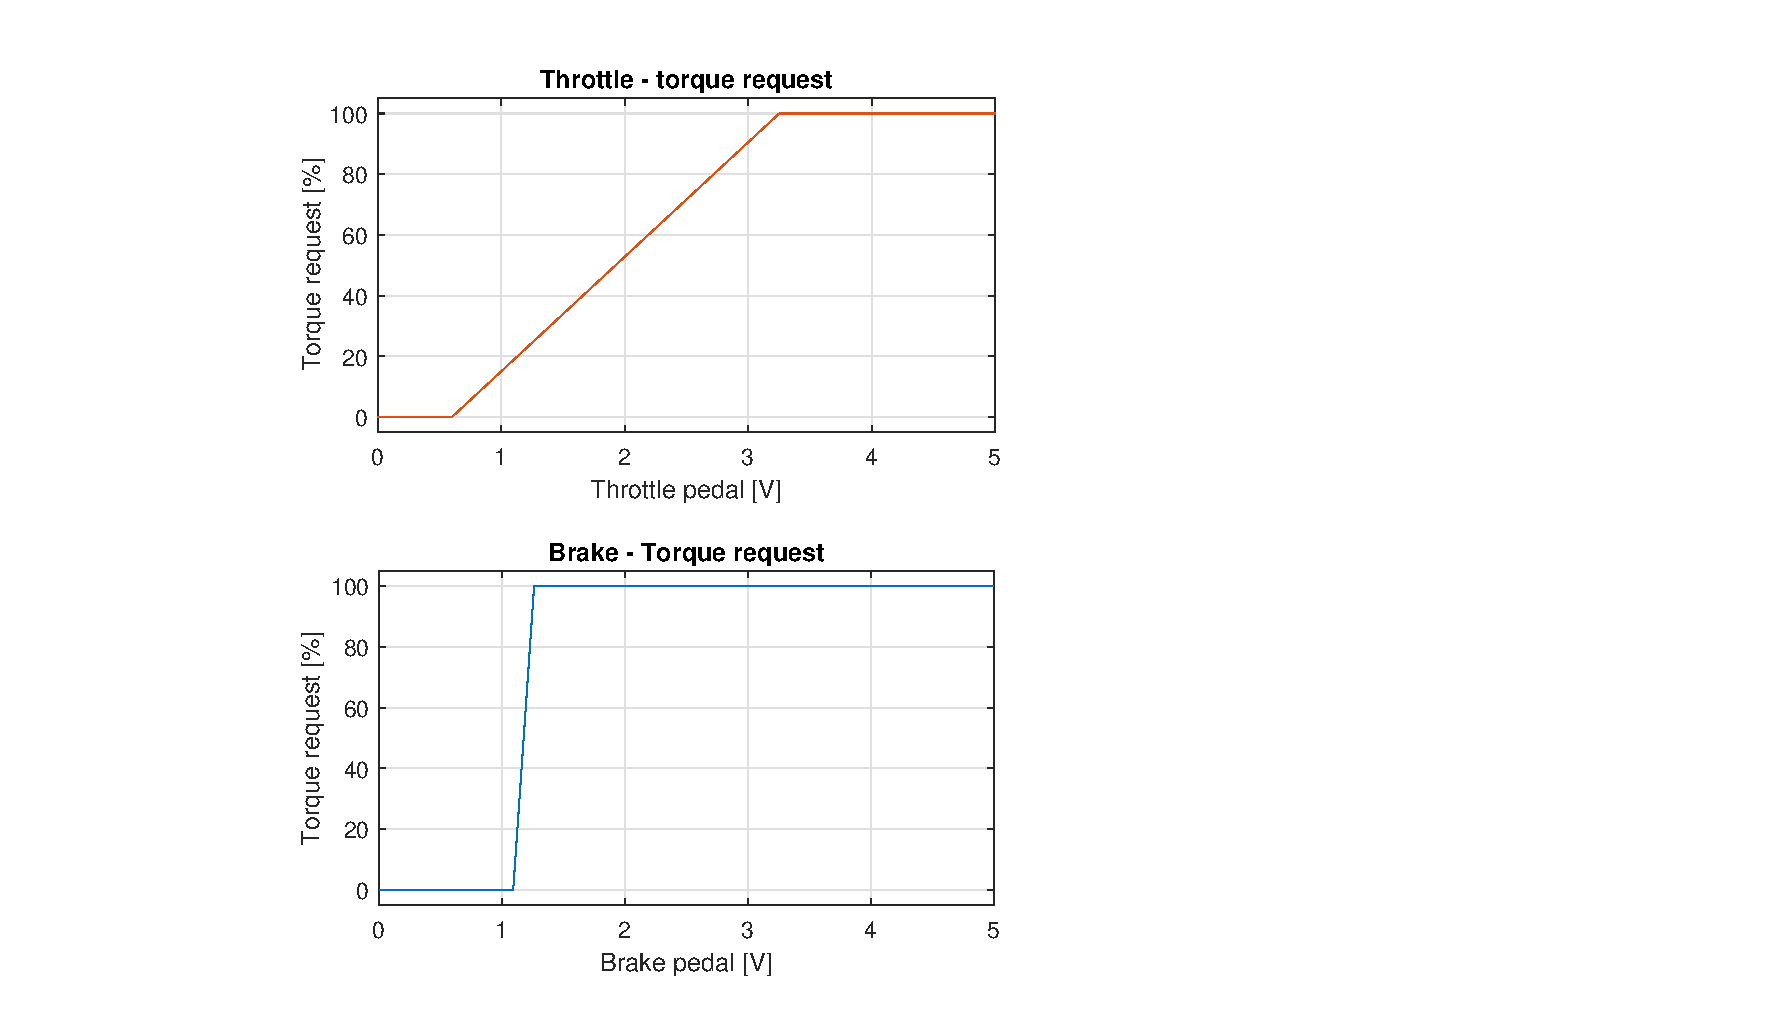
\includegraphics[scale=0.8]{figure/Throttle_Brake_inout.eps}
\caption{Torque request vs throttle and brake pedal voltages}
\label{fig:throt_brake}
\end{figure}

\begin{sidewaysfigure}[hbtp]
\centering
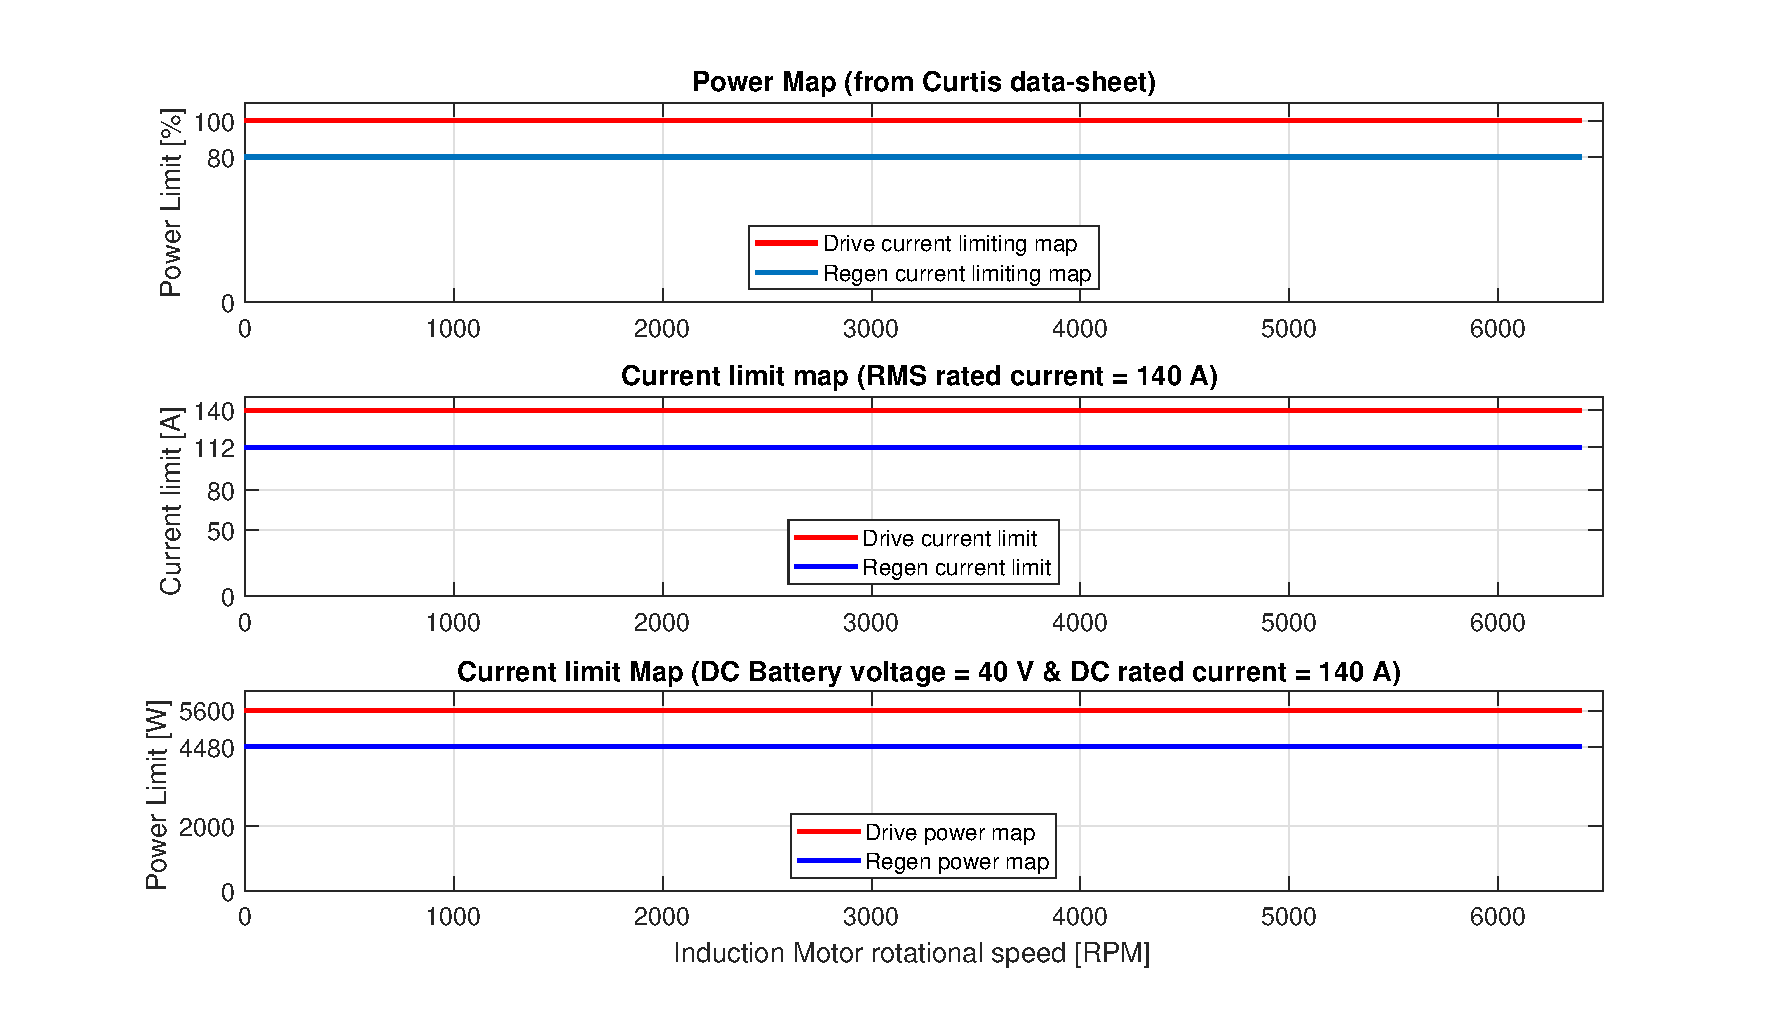
\includegraphics[scale=0.8]{figure/PowerMap.eps}
\caption{Curtis power map}
\label{fig:power_map}
\end{sidewaysfigure}

\textsc{Figure}~\ref{fig:DriveTrai} illustrates the Curtis diagram which receives the throttle and brake commands and provides the 3-phase voltage to the induction motor. It highlights that the AC controller is a black box system which has software access restricted to Mahindra and which has an inaccessible internal processes. It underlines the safety and logical functions ensured by the Curtis and the communication with the \acs{ems} which has also a (software) limited access to Mahindra. 

\begin{figure}[hbtp]
\centering
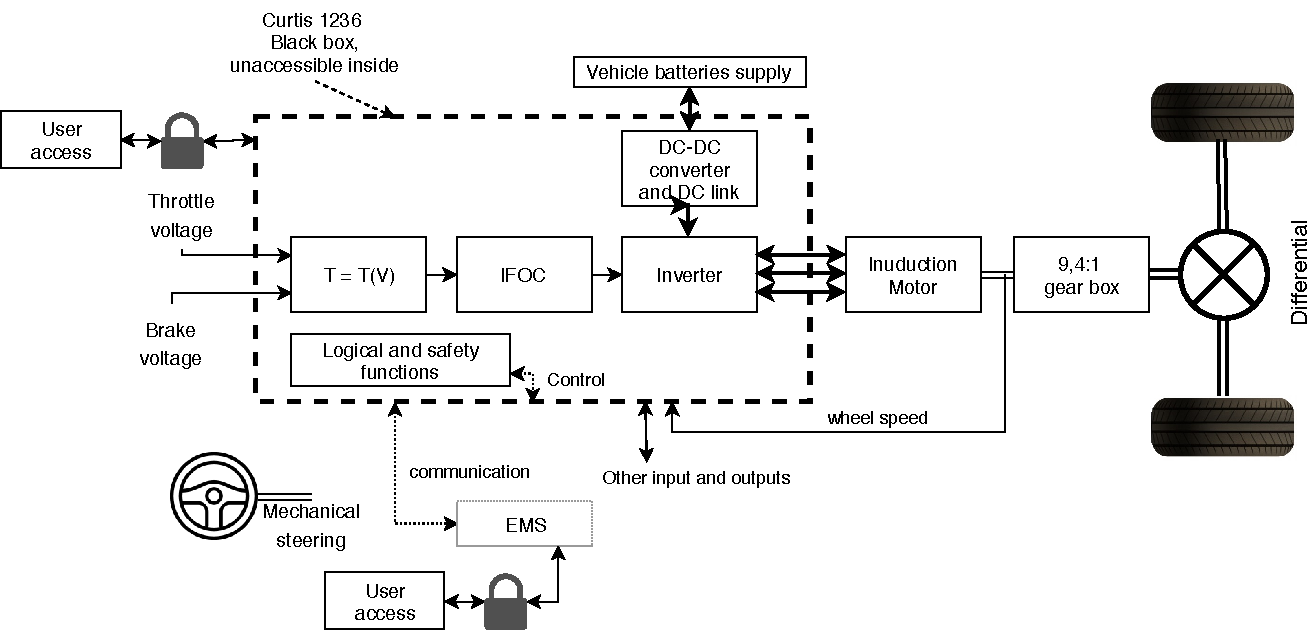
\includegraphics[width=\linewidth]{figure/Drive_trai.pdf}
\caption{Curtis within REVA propulsion system}
\label{fig:DriveTrai}
\end{figure}

\subsection{Batteries}
\begin{itemize}
\item[--] The original REVA batteries were supplying 48~V and had a capacity of 200~~Ah
\item[--] Since the REVA wasn't driving, those were removed for testing 
\item[--] The study in \cite{REVA_anal} had demonstrated the battery cells were damaged and could not supply the REVA anymore
\item[--] The original batteries were hence not re-installed inside the REVA 
\item[--] At the beginning of this master thesis, the REVA had been provided without the original batteries
\item[--] Other batteries were required to supply the REVA which leads to the following section
\end{itemize}

	\section{Battery replacement}
			\subsection{Battery choice}
Since the REVA original batteries were removed during the previous investigation and considered as inoperable, this section discusses the new batteries selection process. The \acs{vub} has 4 batteries used to supply their electric kart project which fits the power requirement for traction need. Below are given their main characteristics~\cite{SuperB}:

\begin{itemize}
\item[--] Model: SB12V160E-ZC\footnote{named later Super B batteries}
\item[--] Rechargeable Lithium Iron Phosphate rechargeable battery
\item[--] Adapted for small vehicle traction requirement or energy storage
\item[--] Internal protection systems
\item[--] Communication interface (\acs{can}Open) for monitoring
\item[--] Nominal voltage 13,2~V
\item[--] Discharge current 480~A
\item[--] Rated capacity  160~Ah (2112~Wh)
\end{itemize}

The Super B batteries are already available at the \acs{vub} which limits the investment cost for the project. Moreover, considering the provided characteristics, such batteries fit the REVA supplying requirement; the discharge current of 480~A complies with the Curtis~1236 operating current (140~A DC). 

Additionally, the Curtis 1236 has a nominal voltage operating range comprised in $[36\:-\:48]$~V \footnote{It will be highlighted later that the nominal battery voltage range $[36;48]$~V is not the configured battery voltage of the Curtis which have been configured at 50~V}. Therefore, 3 of the 4 available batteries were installed in order to stay in the Curtis operating  range; meaning 40~V will by provided to the vehicle by connecting 3 Super B in series. 

It is important to highlight that the original batteries capacity was rated at 200~Ah with a supply voltage of 48 V. Comparatively, the new battery choice have a capacity of 160~Ah and could supply around $40$~V. Thus, a measurement phase was performed to analyze if the Super B batteries were able to supply the REVA properly.  

		\subsection{Plugging the super B batteries}	
The REVA was brought in the laboratory, installed and secured on the \acs{vub}'s roller bench. Actually, their bench allows investigating the REVA without driving it on the road and, additionally, provides vehicle wheel speed and torque measure, plus allows the user to adjust a restitive torque at the roller. The roller bench had been configured in constant torque mode, thus the roller bench adjusts its roller speed in order to keep the torque constant. 

The 3 super B batteries have been plugged in series providing approximately 40~V. Moreover, 2 safety equipment have been added to the setup: 
\begin{itemize}
\item[--] One mechanical switch allowing to connect and disconnect the new battery pack from the vehicle, independently of the vehicle main relay SW180\footnote{refereed as SW 180, the model of the relay)}. Since the vehicle will be modified or manipulated, the switch is a visual clue to avoid working under voltage. Moreover, it permits a safety disconnection if required.  Since there was no available switch supporting more than 100~A, a 3-phase switch supporting 100~A per phase with the input and output terminal short-circuited\footnote{thus each phase shares the current flowing from the batteries to the REVA} was used (\textsc{figure}~\ref{fig:switch_fuse}).
\item[--]  A 200~A fuse, which protects the REVA from undesired over-currents was wired to the switch. 
\end{itemize}

To avoid having the REVA under a positive potential once disconnected (switch opened), the switch and the fuse have been connected to the positive battery pack terminal. In this, case the fuse has been connected after the switch, however it would have been wiser to connect it right after the power source, hence power supply would be protected from the switch as well. Fortunately, the batteries have internal protections. The fuse was then connected to the positive terminal of the main (contact) relay while the ground of vehicle have been connected to battery pack negative terminal, as shown in \textsc{figure}~\ref{fig:pano} and~\ref{fig:meas_setp}. 

\begin{figure}[hbtp]
\centering
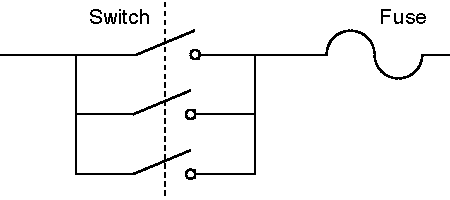
\includegraphics[scale=0.8]{figure/Connectors.pdf}
\caption{Switch and fuse}
\label{fig:switch_fuse}
\end{figure}

\begin{figure}[hbtp]
\centering
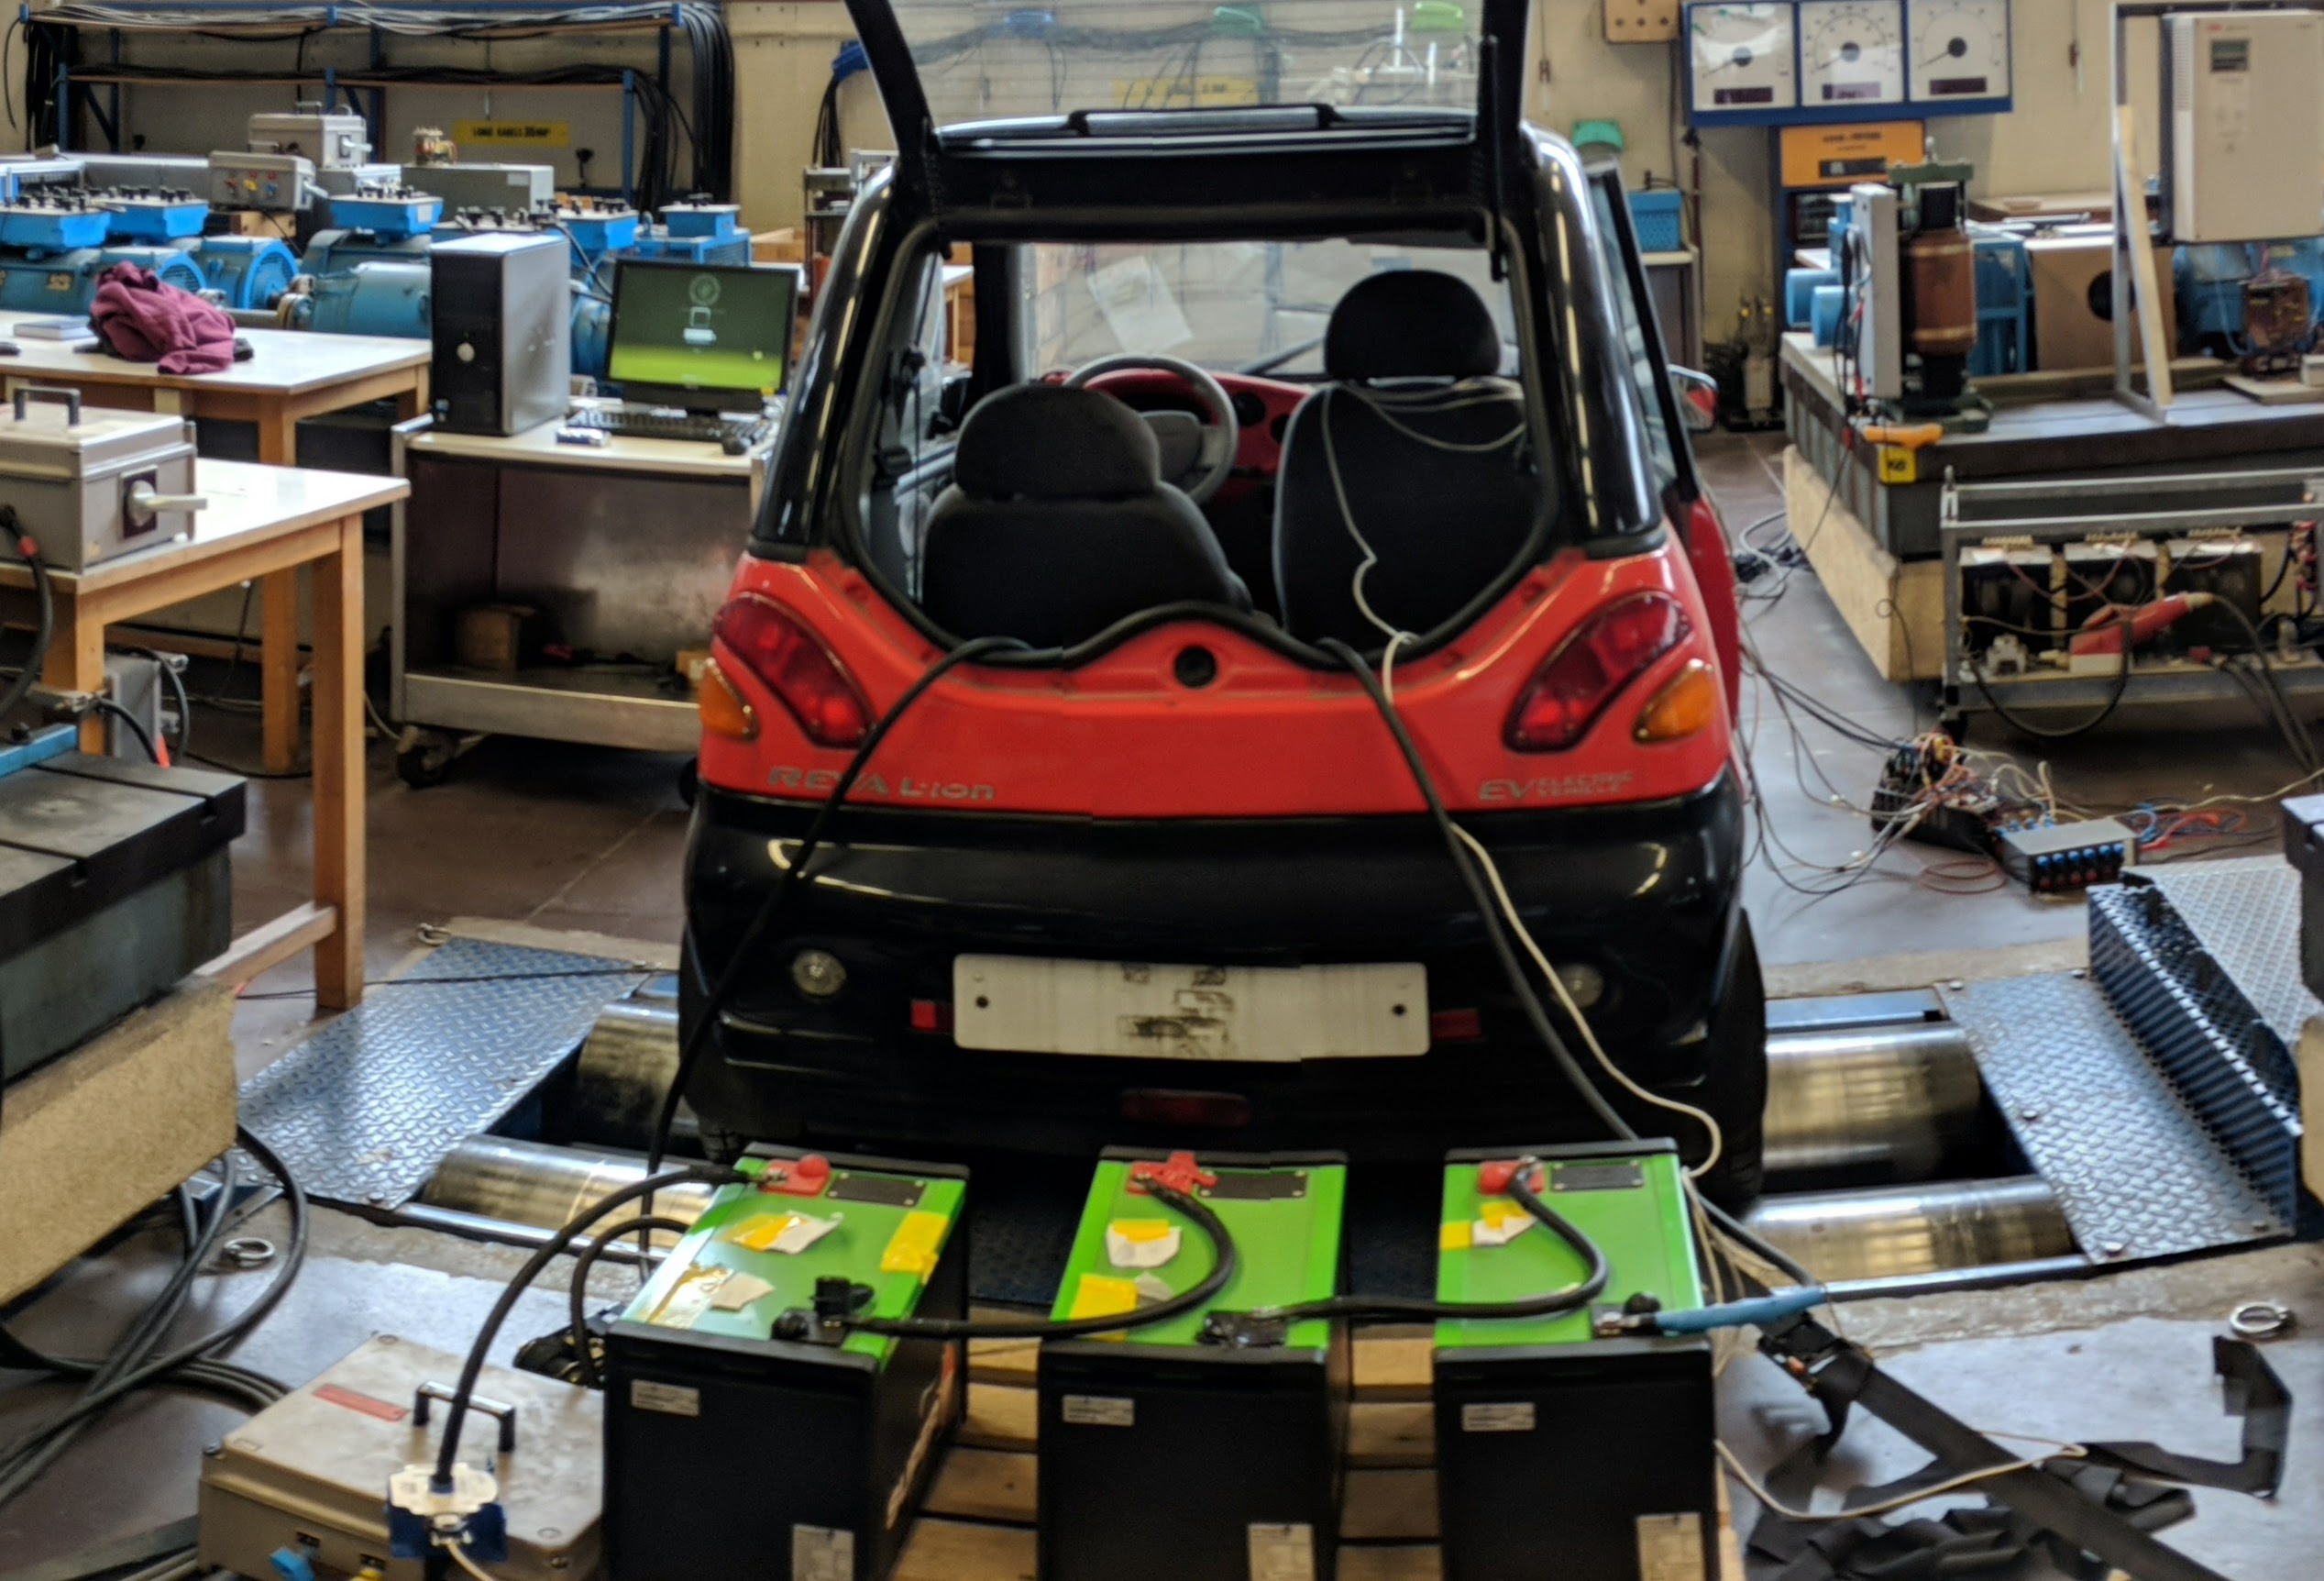
\includegraphics[width=\linewidth]{figure/pano_reva.jpg}
\caption{REVA battery setup on the roller bench}
\label{fig:pano}
\end{figure}

\begin{figure}[hbtp]
\centering
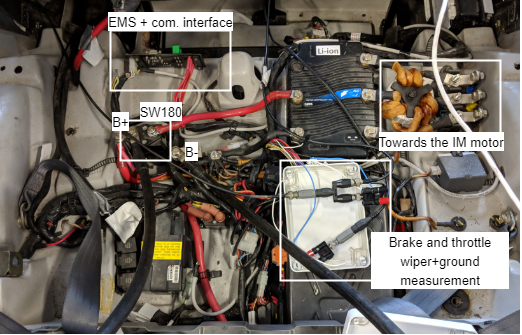
\includegraphics[width=\linewidth]{figure/connect.png}
\caption{REVA components}
\label{fig:connectpng}
\end{figure}

			\subsection{Throttle and break pedals access}
As stated in~\cite{Curtis_User_Manual} and annex~\ref{s:REVACurtisParam}, the pedal of the REVA are 3-wires potentiometers\footnote{in~\cite{Curtis_User_Manual} and~\ref{s:REVACurtisParam}, such potentiometer are referred as Throttle (or Brake) Type 2}; the more one pushes the pedal, the higher the resistance will be and the higher the wiper voltage will be. Each potentiometer is connected to the Curtis 1236 trough its port (shown \textsc{figure}~\ref{fig:Curtisand_port}) which supplies them and measure the voltage command at the wiper. 

In order to access the measures of the pedals, the cables incoming to the Curtis connector have been cut as illustrated on \textsc{figure}~\ref{fig:pot}. The low potential (18), the brake wiper (17), and the Throttle wiper (16) have been cut, and by-passed using additional connectors and cables. Using an adapter, the measure can be accessed using coaxial cables. 

\begin{figure}[H]
\centering
 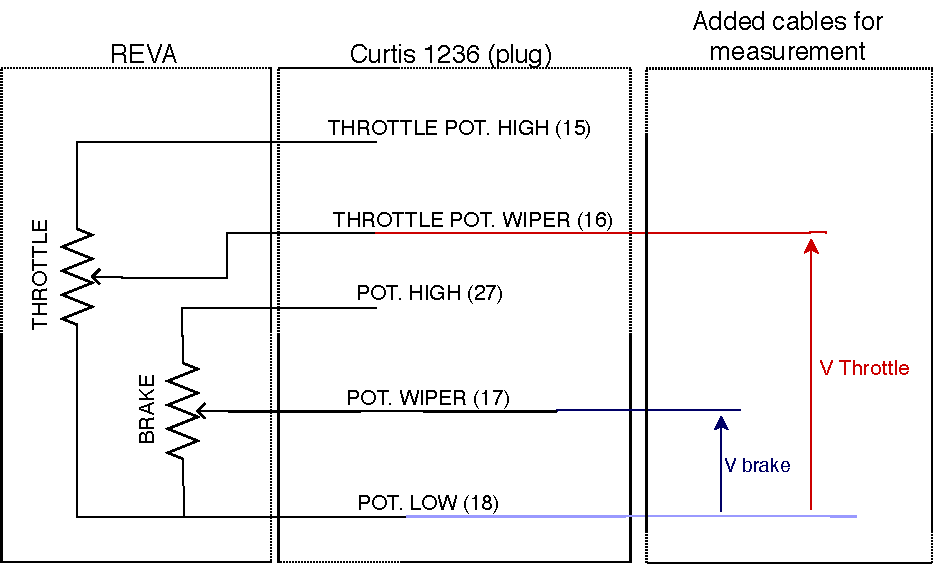
\includegraphics[scale=0.70]{figure/By-pass.pdf}
\caption{Pedal Potentiometer (adapted from~\cite{Curtis_User_Manual})}
\label{fig:pot}
\end{figure} 

\begin{figure}[htbp]
    \centering
    \begin{subfigure}[b]{0.5\textwidth}
        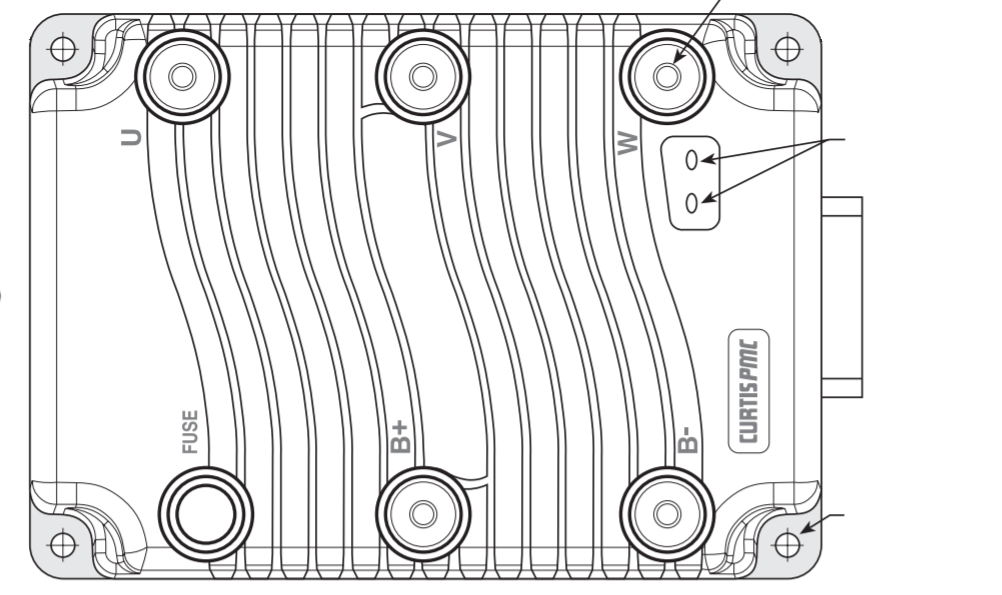
\includegraphics[scale=0.45]{figure/Curtis.png}
        \caption{}
        \label{fig:Curtis}
    \end{subfigure}
    \hfill
    \begin{subfigure}[b]{0.35\textwidth}
        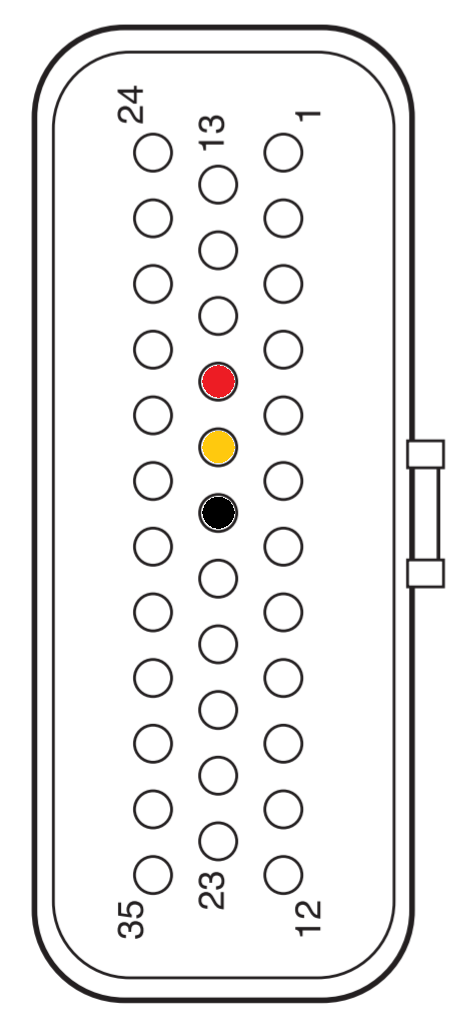
\includegraphics[scale=0.20]{figure/Curtis_Motor_Controller.png}
        \caption{Curtis 1236 Connector. Black (18) Pot Low. Yellow (17) Brake Pot. Wiper. Red (16) Throttle Pot. Wiper}
        \label{fig:Curtis_connector}
    \end{subfigure}
    \caption{Motor Controller - Curtis 1236~\cite{Curtis_User_Manual}}
    \label{fig:Curtisand_port}
\end{figure}

\begin{table}[htbp]
\newcolumntype{Y}{>{\centering\arraybackslash}X}
\begin{tabularx}{\textwidth}{ |Y|Y|Y| }
\hline
\textbf{Measure} & \textbf{Device} & \textbf{Ratio} \\
\hline \hline
Battery current & LEM ITB-300s & 1 V : 2000 A \\
\hline
Battery voltage & LEM CV3-500  & 1 V : 50 V \\
\hline
Line current    & Fluke i400s  & 1 mV : A \\
\hline
Line voltage    & LEM CV3-1000 & 1 V : 100 V \\
\hline
Phase voltage   & LEM CV3-500 & 1 V : 50 V\\
\hline
Pedal signal & Direct measure & 1 V : 1 V \\
\hline
Brake signal & Direct measure & 1 V : 1 V \\
\hline
Roller speed & Direct measure & 1 V : 5,2 rad/s\\
\hline
Roller speed (voltage divider) & Elditest electronic GE 8100 & 1 V : 20 V\\
\hline
Roller torque & Direct measure & 1 V : 941 N\\
\hline
\end{tabularx}
\caption{Measurement devices and their ratio}
\label{table:devices}
\end{table}

		\subsection{Data acquisition}
The data acquisition is realized using a \acf{ni} \acf{crio} which has been programmed as a real-time measurement tool. The cRIO has 20 inputs for coaxial wires and accepts a signal range between 1 and 10~V. The number of inputs is sufficient for this experiment, and each signal measure fits within the voltage range except the speed measure from the roller bench which requires a voltage divider to fit within the required range. Each measurement, its related device and transformation ratio is provided in \textsc{table}~\ref{table:devices}. The measurement frequency has been set at 1000~Samples/s which should satisfy the measurement objective. 

\textsc{Figure}~\ref{fig:meas_setp} illustrates the measurement setup. Some of the measurements devices required a 30~V DC serial-power supply which has been omitted on this figure. Lastly, the process for acquiring the data using the \acs{crio} is described in Annex~\ref{sec:cRIOdataAcq}. The \acs{crio} provides the data within TDMS file format from \acs{ni} which requires the usage of their \acs{ni} DIAdem software. 

\begin{figure}[htbp]
\centering
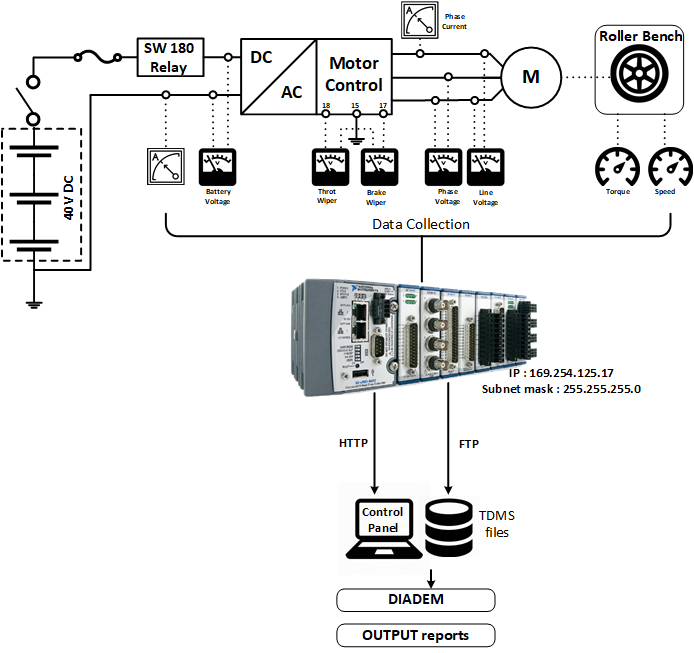
\includegraphics[scale=0.6]{figure/setup.png}
\caption{Measurement setup}
\label{fig:meas_setp}
\end{figure}

		\subsection{Data Processing}
The raw measured data are not relevant as-is and must be converted into a readable data with the appropriate units. The conversion was made directly using the DIAdem software allowing the user to write VBscripts to automate measurements treatments. A self-made VB script has been written and provided in Annex~\ref{anexe:VBscript}. The script mainly multiplies the raw data by the appropriate ratio, filters them, arrange the data properties and plots multiple diagrams. 
			\subsubsection*{Speed conversion}
The analogical speed measure is a sine wave with an amplitude and frequency varying with the rotational speed. The transformation ratio between the speed and the amplitude is 5,2 rad/s for 1 V. The computation of the speed is based on its Root Mean Squared (RMS) value computed thanks to a related DIAdem function. 

The equation below converts the RMS value of $V_{meas}$ from the roller bench rotational speed into the REVA longitudinal velocity in kilometer per hour. Where 20 stands for the voltage divider ratio, $0,159$ is the roller radius and $3,6$ is a ratio factor. 
\begin{equation}
V_{kmh} = V_{meas_{RMS}} * 20 *5,2 * 0,159 * 3,6
\end{equation}
			\subsubsection*{Torque conversion}
The torque at roller bench is given in Newton meter by the equation below where $r_{roll}$ is the radius of the roller, and 941 is a conversion factor; $T_{Nm}$ is the torque at the REVA rear wheels. 
\begin{equation}
T_{Nm} = T_{meas} * 941 * r_{roll} = T_{meas} * 941 * 0,159 
\end{equation}

			\subsubsection*{Filtering}
Additionally, the measurements noise is filtered using within the VBscrpit using low-pass filter which frequency has been chosen for the measure (typically around $0,05$~Hz). 
	\section{Data analysis}
The REVA does not drive correctly while using the new Super B batteries, this section aims is to analyze and diagnose the problem source. Multiple data measurements have been recorded however only few measurements are provided here to illustrate the REVA's behavior while the other are omitted. Nevertheless, they can be downloaded at...
	\subsection{Issue 1: reduced torque}

\begin{figure}[hbtp]
\centering
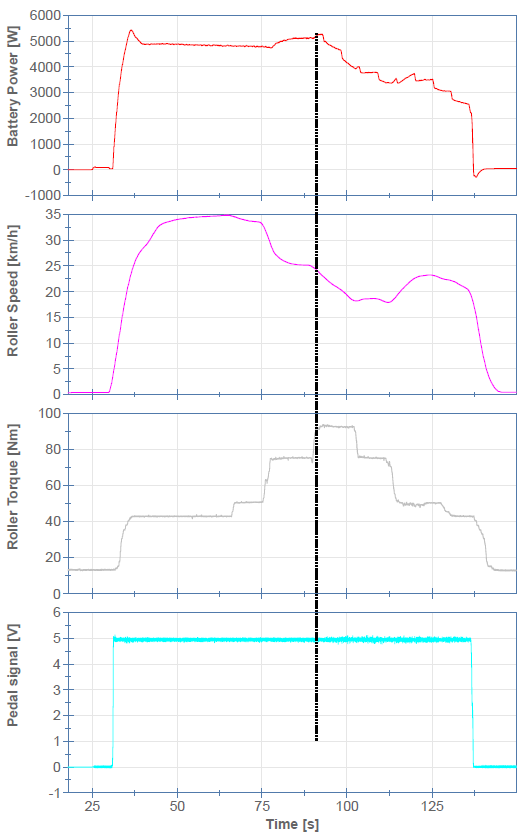
\includegraphics[scale=1]{figure/full_throt_exp.png}
\caption{Full throttle response of the REVA}
\label{fig:data_exp1}
\end{figure}

The REVA was submitted to a full throttle experiment with the results provided in \textsc{figure}~\ref{fig:data_exp1}. While the throttle pedal was maintained fully pushed, the resistive torque was increased by steps using the roller bench. The following observations can be made: 
\begin{itemize}
\item[--] As expected from \textsc{figure}~\ref{fig:throt_brake}, the throttle pedal reaches 5~V, and the torque requested by the driver causes the REVA to accelerate. 
\item[--] While accelerating from 0 to 35~km/h, the battery power reaches 5500~W and then stabilizes at 5000~W. 
\item[--] While the torque is kept minimum (41~Nm), the REVA accelerates up to 35~km/h, which is not the maximum speed of 80~km/h expected from the vehicle data-sheet, and, the battery power remain steady at 5000~W. 
\item[--] The battery power remains at 5000~W when the torque is increased from 41~Nm to 50~Nm, however the speed decreases to 32~km/h. 
\item[--] Once the torque have been increased to 77~Nm, the battery power increases to 5100~W and the REVA's speed decreases to 25~km/h. 
\item[--] When going above a resitive torque of 77~Nm, (dashed line), the vehicle speed decreases. While the torque is increasing, the battery power increases for a small amount of time, it then decreases. 
\item[--] Even if the resistive torque is reduced, the battery power does not return into a steady value. The restive torque is reduced, however the speed does not stabilize nor the battery power. 
\end{itemize}

The battery voltage and current measurements (from the same experiment as above) are provided in \textsc{figure}~\ref{fig:SupVoltCur}, and \textsc{figure}~\ref{fig:SupVoltCurZoom} zooms on the vehicle accelerating period. The following observation can be made: 
\begin{itemize}
\item[--] The unloaded battery voltage (vehicle switched on but stand-still) is measured at 40,3~V while the loaded battery voltage decreases to 36,7~V (vehicle in motion) and remains mostly steady during the entire experiment. 
\item[--] When the vehicle is in motion, a steady state current of 131~A is provided by the batteries. When accelerating, the current reaches 150~A temporarily. 
\item[--] Once the torque reaches 77~Nm, the current goes up to 140~A, and at 92~Nm, the current shortly reaches 148~A then decreases permanently. 
\end{itemize}

\begin{figure}[hbtp]
\centering
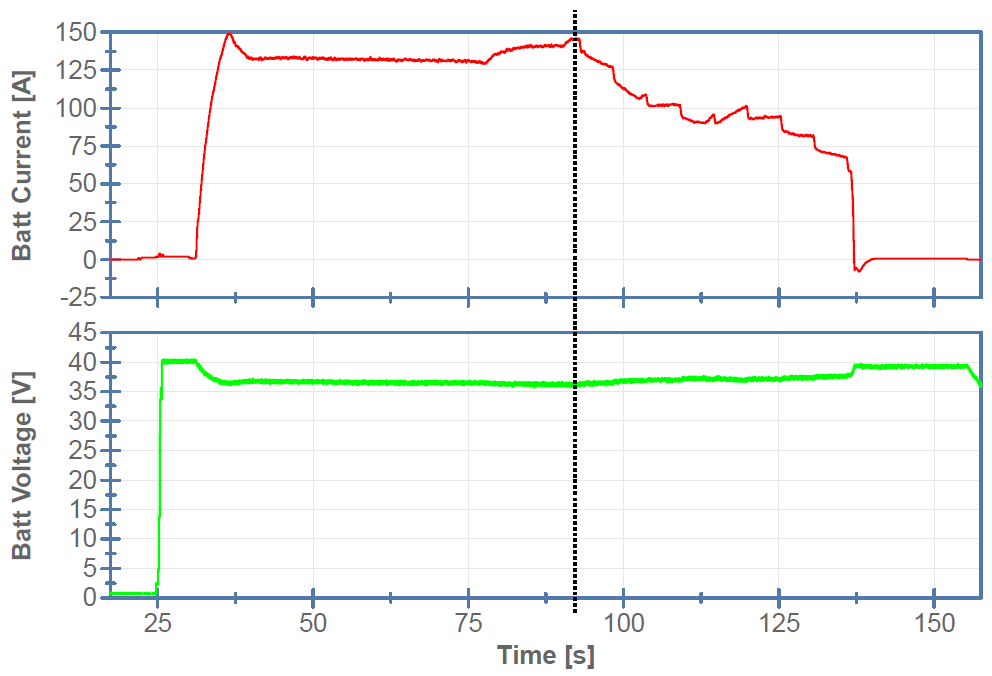
\includegraphics[width=\linewidth]{figure/Bat_current_graph.png}
\caption{Super B supplied voltage and current}
\label{fig:SupVoltCur}
\end{figure}

\begin{figure}[hbtp]
\centering
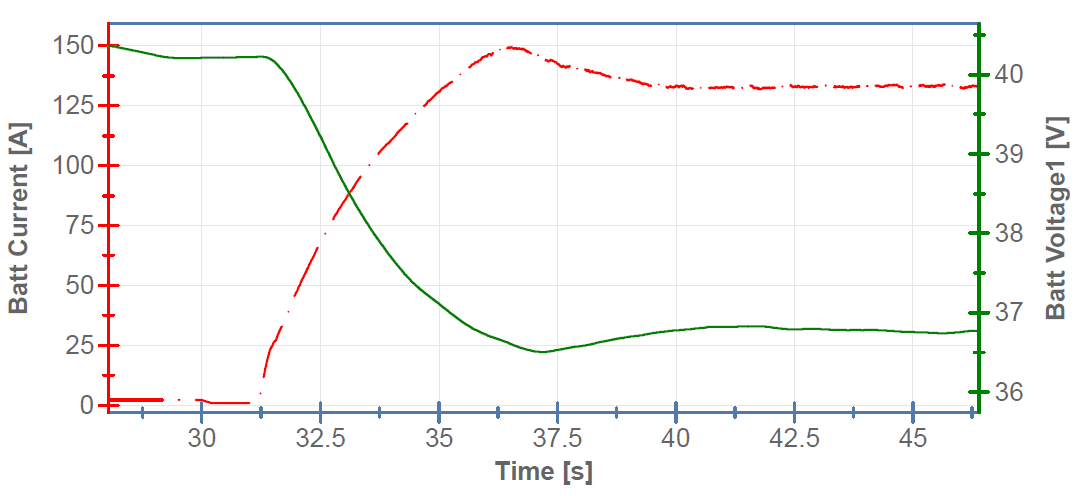
\includegraphics[width=\linewidth]{figure/Bat_current_graph_zoom.png}
\caption{Accelerating Super B supplied voltage (line) and current (dashed)}
\label{fig:SupVoltCurZoom}
\end{figure}

		\subsubsection{Diagnostic 1: undervoltage issue}
While recording the experiment data, the reading of the Curtis status LEDs provided a 23 error code which is related to an undervoltage power suply reducing the available motor torque (\textsc{table}~\ref{tab:errorCode}). The possible causes of this error are provided in \textsc{table}~\ref{tab:ReducedT_cause} as their verification. 

As described in \textsc{table}~\ref{tab:ReducedT_cause}, the motor controller does not operate in its operating region. Indeed, the nominal voltage have been misread in the Curtis documentation which provides two information: 
\begin{itemize}
\item[--] One mentioning the nominal battery voltage range is 36-48~V which have been used until now
\item[--] Another mentioning an internal Curtis parameter which must be tuned according the batteries. Annex~\ref{s:REVACurtisParam} provides all internal parameters, and especially the nominal battery voltage which have been tuned at 50~V. 
\end{itemize}

All Curtis voltage related parameters have been summarized in \textsc{figure}~\ref{fig:CurtisVoltLevel} as well as the Super B voltage operating region\footnote{ 36,5~V when the batteries are loaded, 42~V when the batteries are fully charged, and 40,8~V unloaded}. This figure highlights that the operating voltage of the REVA, does not match the supply voltage of the used super B batteries and therefore explains the 23 error code. The limited available torque explains the observations of the left part of the dashed line (limited torque involves reduced speed) in \textsc{figure}~\ref{fig:data_exp1}. Additionally, the power and current observation compiles with the power and current expectation provided earlier on the power map (\textsc{figure}~\ref{fig:power_map}). 

\begin{table}[hbtp]
\newcolumntype{Y}{>{\centering\arraybackslash}X} 
\begin{tabularx}{\textwidth}{ |Y|Y|Y| }
\hline
Error code & Name & Effect \\
\hline \hline
23  & Undervoltage Cutback & Reduced drive torque \\
\hline
\end{tabularx}
\caption{Curtis 1236: error code 23}
\label{tab:errorCode}
\end{table}	

\begin{table}[hbtp]
\newcolumntype{Y}{>{\centering\arraybackslash}X}
\begin{tabularx}{\textwidth}{ |Y|Y| }
\hline
Cause of Undervoltage & Check  \\
\hline \hline
Normal operation. Fault shows that the batteries need recharging. Controller is performance limited at this voltage.  & Once verified, the REVA was not operating under its nominal voltage (see \textsc{figure}~\ref{fig:CurtisVoltLevel}  \\
\hline
Battery parameters are misadjusted.   & True, the internal Curtis Battery parameters are not adjusted to the new batteries  \\
\hline
Non-controller system drain on battery.    & No  \\
\hline
Battery resistance too high.   & Unknown required resistance  \\
\hline
Battery disconnected while driving.   & No  \\
\hline
See Monitor menu » Battery: Capacitor Voltage.    & Parameters not accessible  \\
\hline
Blown B+ fuse or main contactor did not close.   & No  \\
\hline
\end{tabularx}
\caption{Possible Cause of error 23 verification}
\label{tab:ReducedT_cause}
\end{table}		

\begin{figure}[hbtp]
\centering
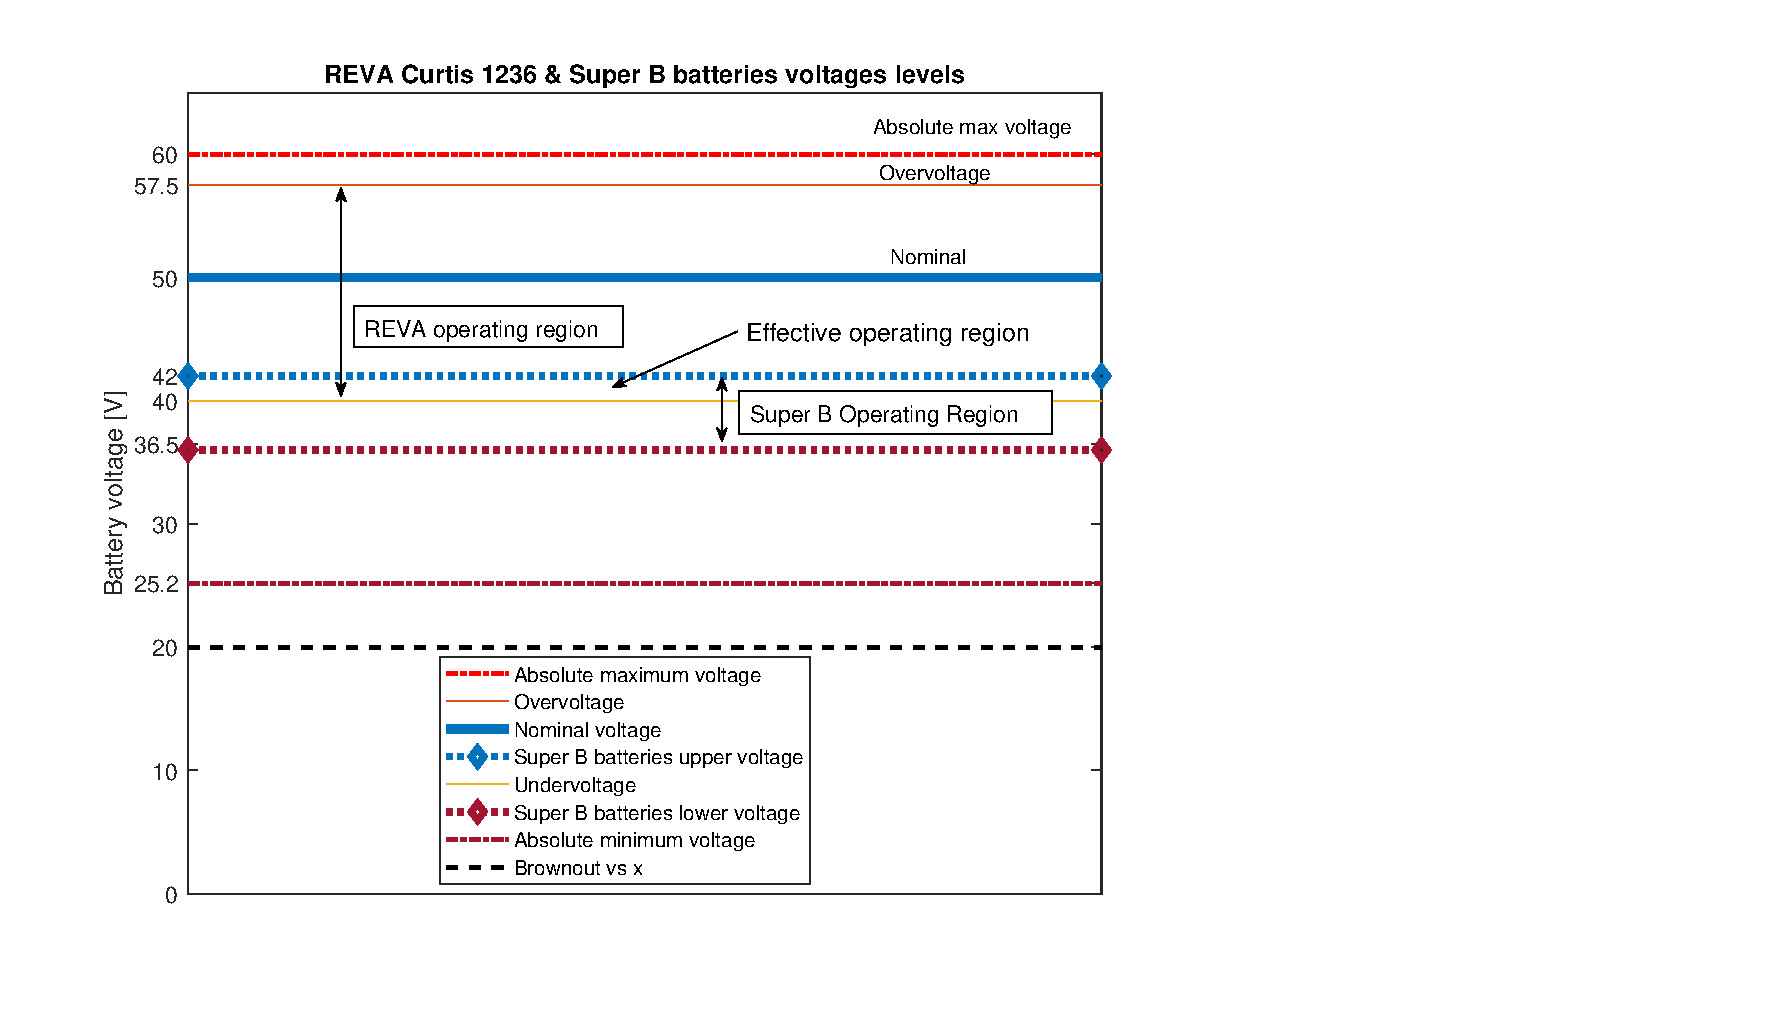
\includegraphics[scale=0.8]{figure/Voltage_levels.eps}
\caption{REVA Curtis 1236 and Super B batteries (3x) voltages levels}
\label{fig:CurtisVoltLevel}
\end{figure}
				\subsubsection{Diagnostic 2: defect mode and safety procedure}
The right part of the experiment illustrated  on \textsc{figure}~\ref{fig:data_exp1} is however unjustified by the 23 error. The current supplied by the batteries decreases independently of the throttle command. This phenomenon happened multiple times at various speed, independently of the restive torque applied. The REVA just seems to work better when low power consumption and struggles at higher power (higher speed or torque). The problem seems however to be caused by an algorithm and not from a component failure otherwise we wouldn't see the clear distinction between left and right data within in \textsc{figure}~\ref{fig:data_exp1}. 

The \acs{ems} measures the batteries voltages and their temperatures to regulate the energy flow while the REVA is being recharged or driven. Most likely, the \acs{ems} would cooperate with the Curtis for managing those flow. Since the original batteries were replaced by 3 Super B, the \acs{ems} algorithms may not be parameterized to work with those (as it happened with the Curtis) and a safety procedure which overrules the Curtis commands inquires the motor controller to reduce its output current until it reaches 0~A; reducing the motor torque and slowing down the REVA. Nevertheless, due to the lack of data-sheet about the \acs{ems}, there is not literal evidence about this assumption. However, the Curtis 1236 surely monitors the batteries and might enable this safety mode. Even if the component causing this safety mode is unidentified, it is most likely due to an inappropriate power supply. Thus, an experimentation using a power supply within the required voltage and current ranges is required. 

		\subsection{Issue 2: Non-operating at nominal voltage}
As the nominal voltage of the Curtis 1236 has been parametrized at 50~V, the fourth Super~B has been added in series to the 3 others in order to supply 53~V to the REVA. The supplied voltage is hence comprised within the operating range of the Curtis 1236 given above.  The REVA was then tested using the new battery set, and the following observation was made: 
\begin{itemize}
\item[--] REVA starts normally
\item[--] No status error from the Curtis 1236
\item[--] While driving the REVA was generating abnormal noises
\item[--] The wheel speed was not reaching a steady state value and sounds to oscillate around an average speed. 
\end{itemize}

Because of the REVA abnormal behavior when supplied by 53~V, no experiment has been recorded with this configuration. 
			\subsubsection{Diagnostic: damaged battery}
In section~\ref{sec:experiment_issue} is concluded that the fourth battery used was previously damaged which most likely caused this abnormal behavior. It is therefore not possible to conclude if the REVA would operate normally if supplied with the correct source and requires an additional experiment with an appropriate power supply. 

	\section{Conclusion}
This chapter objective was to present, analyze and determine if the Super B batteries are able to supply the REVA. 

The REVAi from Mahindra Electric is an \acf{ev} using an \acf{im} controlled by an Curtis 1236 motor drive. Despite knowing the power maps of the motor, its data-sheet remained inaccessible and the \acs{im} parameters are missing. The Curtis 1236 is a motor controller which generates, using the throttle and brake inputs, the appropriate AC signals supplying the \acs{im} from the DC batteries. The Curtis uses an \acf{ifoc} based algorithm which has additional safety procedures over-layers. This device is a black box process where the main internal sub-processes principles are known but are inaccessible and details about those sub-processes are unprovided. The Curtis is a reprogrammable motor drive meaning a finite set of parameters can be tuned using Curtis tools (a software and handler programmer). However, as stated by Curtis himslef, the REVA Curtis 1236 has a restricted access for non-Mahindra user and the Curtis cannot be reprogrammed\footnote{Curtis England statement}

However, the Curtis 1236 parameters are provided in annex~\ref{s:REVACurtisParam}, which has outlined the power map (7000~W), the maximum currents (140~A), and the operating REVA voltage range (40 to 57,5~V, 50~V nominal). Moreover, it mentions the \acs{ifoc} is set in torque control mode meaning the throttle and brake commands of the Curtis are interpreted as torque requests. 

The REVA \acf{ems} can be accessed through the communication interface using iEMS software. The software requires logs provided by Mahindra who has restricted the access to vehicle data. The \acf{can} port remains available and the \acs{can} data frames may be hacked.  

As one cell of the original batteries was broken, new Super B batteries were plugged to the REVA as replacement. A testing procedure was performed which allowed to identify two major problems; (1) the new supply 3x Super B power provides 37,5~V (loaded) which out of the operating range causing the REVA to perform with a reduced driving torque. (2) The Curtis 1236 and \acs{ems} parameters are not calibrated according to the new battery which enables randomly a safety procedure reducing the current flow towards the \acs{im} reducing its torque until the REVA stops. However, those observations are not REVA dysfunctions but a normal protection against abnormal situations. An extra measurement of the REVA using an adequate power supply is required to settle the REVA statement.   

\acfp{av} require both being steer-by-wire and throttle/brake-by-wire to ensure the vehicle actuation by electric signals. The REVA steering is ensured by a mechanical shaft disabling the possibilities to achieve the lateral control required by an \acs{av}. It is however throttle and brake by wires which enables the longitudinal control (or speed tracking). If the Curtis 1236 is to be used for achieving the speed tracking, the device is constrained to work in torque control mode. 

\chapter{Speed control \label{chap:speed_control}}	
One of the main achievement in highly automated driving is the speed and steering self-control. Indeed, after the vehicle \acf{dmu} has predicted and generated a model of the path, the vehicle must physically follow those computed references according to a process named \textit{motion control}. Such process is the set of methods applied by the vehicle to achieve the speed and steering reference following. Based on the vehicle state, those methods compute and send commands to the electronic actuator of the vehicle. A vehicle can be actuated by those commands in two fashions; actuating the gas or brake pedals ensures longitudinal (or speed) control, while actuating the steering wheel enables the lateral (or steering) motion control of the vehicle. 

In chapter~\ref{chap:reva} we have discussed the state of the REVA electric vehicle prototyping platform. The steering shaft is mechanically linked to the wheels and thus is not actuated by an \acf{ecu}. Therefore, the lateral control is not achievable in the current vehicle state. However, the gas and brake pedals are potentiometer generating voltage signals commanding the motor controller. Hence, by unplugging those devices, and replacing them by a self-made voltage control unit, the longitudinal control is practically achievable. 

This chapter objective is to illustrate the process of achieving the longitudinal control for the REVA prototype on the \acs{vub}'s roller bench. It describes the REVA system and the strategy adopted to achieve the longitudinal speed control. Next, among multiple control methods, it selects the most appropriate one for this case study and proposes a practical software and hardware implementation using the REVA prototype. 

\textit{Nota bene:} In chapter 3, we have concluded that the prototyping platform components were uncalibrated with regard to the new power supply making the platform not working normally. However, when starting the development of the speed controller, this statement wasn't made proven and the conclusion about the REVA state has been the result an iterative procedure while working on it. 

	\section{Longitudinal speed control}
Longitudinal control is part of the automated vehicle motion control which realizes the tracking of the \acs{dmu} speed reference within the surrounding of the vehicle (\textsc{figure}~\ref{fig:DMU_Speed}). This chapter objective is to build a speed controller for the REVA capable of tracking this time-varying speed reference. 

\begin{figure}[hbtp]
\centering
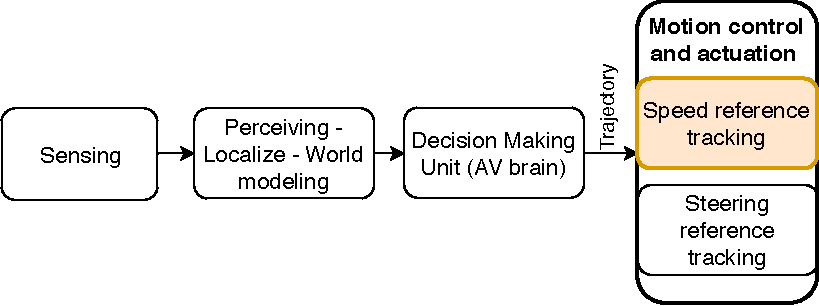
\includegraphics[scale=0.8]{figure/AV_frame_locate.pdf}
\caption{\acs{av} motion control}
\label{fig:DMU_Speed}
\end{figure}

The actual speed must follow as close as possible the reference while overshoot and static error must be reduced. The dynamic of the controlled system must be sufficient to react as a human driver would operate in the same conditions. Moreover, the regulated system must demonstrate robustness with regard to external perturbations\footnote{such as wind, road slopes, rolling resistance, etc.}. The conception and implementation must be cost effective by using as much as possible the available materials of the \acs{vub}'s laboratory. This section's aim is to describe the methodology and the choices made to develop such a controller. 
		\subsection{System description}
Without the automated longitudinal control, the speed tracking task is left to the driver. He evaluates the speed at which he wants to drive, then he estimates the appropriate actions to follow his mental velocity reference. Based on the difference between the wanted and the actual speed, the driver pushes or releases the gas or brake pedals which modulates the traction effort generated by the vehicle. The human acts therefore as the controller; he computes the difference between the desired and the actual speed (respectively the set point and the process value) which provides the error estimation. According to this, the driver actuates the pedals to track the desired velocity by requesting a torque modulation from the vehicle. The block diagram of the described human speed regulation loop is provided in \textsc{figure}~\ref{fig:control_loop}. 

\begin{figure}[hbtp]
\centering
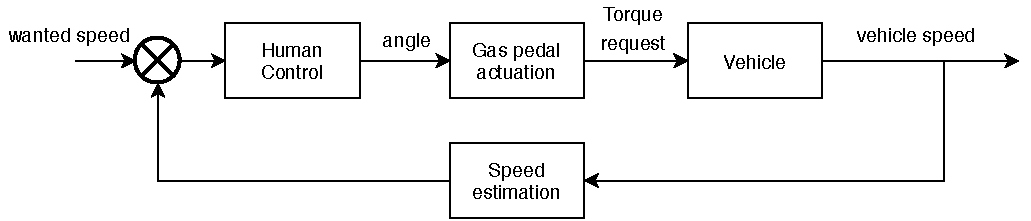
\includegraphics[scale=0.85]{figure/control_loop.pdf}
\caption{Human control loop}
\label{fig:control_loop}
\end{figure}

The actual \textit{vehicle} block represents the REVA and comprises multiple subsystems of the car power train. First, the motor drive\footnote{Motor drive, drive, and motor controller are used as synonyms} (or Curtis\footnote{REVA motor drive manufacturer} 1236\footnote{Curtis motor drive model}), receives the voltage commands generated at the pedals which effects its behavior. Given a brake signal, the Curtis actuates the mechanical drum brakes and starts the regenerative braking phase. Oppositely, a throttle signal is converted into a torque request which is internally provided to the embedded \acf{ifoc} algorithm of the Curtis. An \acs{ifoc} is a control method that modulates the torque-speed curve of the attached electric motor. To do so, from the motor speed measure and the pedal torque request, its algorithms compute the appropriate command signal sequence provided to the inverter. This device, converts the \acs{dc} power from the batteries into a 3-phase AC signal for the REVA induction motor. Having a modular control sequence triggering the inverter allows to modulate the \acs{ac} voltage and current waveform provided to the induction motor, which in return modulates the electric motor torque and therefore the vehicle wheels torque. Secondly, the provided torque at the wheels brings the REVA into motion, depending on the longitudinal external dynamic behavior of the vehicle, the car will move at a certain speed. Each mechanical or electrical links such as the differential can be also considered as subsystems, but will be neglected in this case. Therefore, the \textit{vehicle} system comprises 5 physical subsystems; the motor controller (Curtis 1236), with (1) its command to torque conversion,  (2) its \acs{ifoc} and (3) associated inverter, then (4) the \acf{im} and finally (5) the external vehicle dynamic applied on the REVA. The Curtis 1236 is end-to-end device which is considered as a black box system (\textsc{figure}~\ref{fig:CutisSys}); its working principle is known but the internal components are inaccessible. Finally, the speed control loop of the REVA is provided in \textsc{figure}~\ref{fig:control_loop_detailed}. 

\begin{figure}[hbtp]
\centering
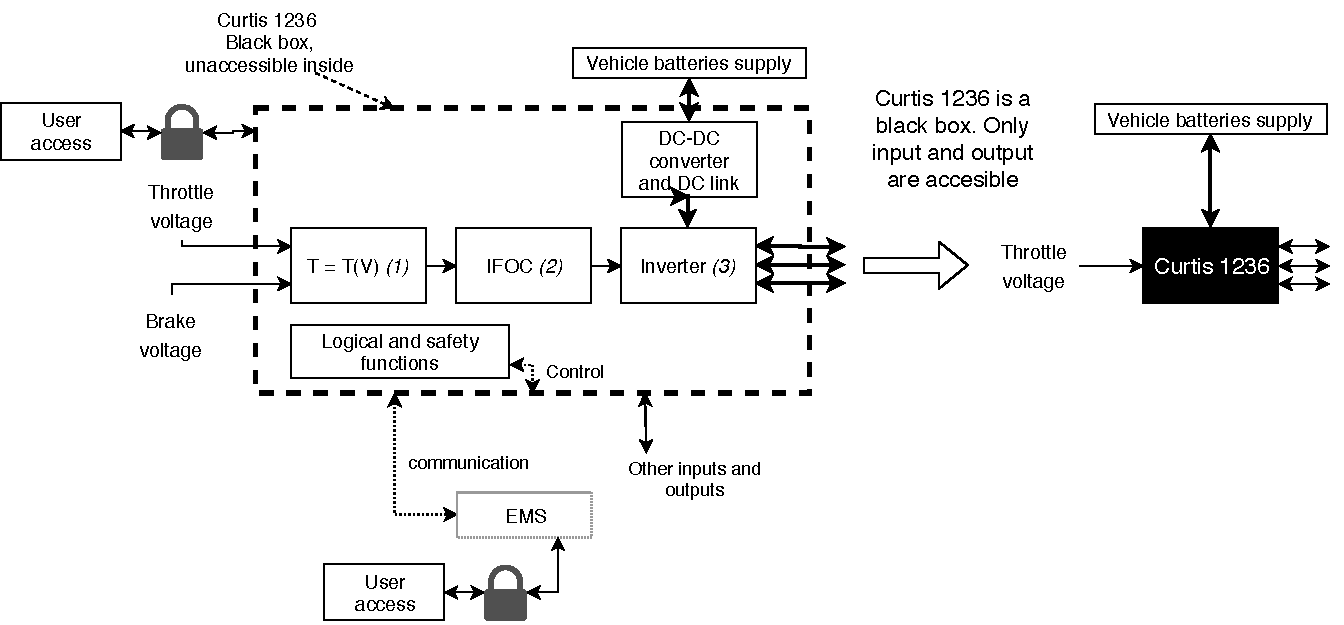
\includegraphics[width=\linewidth]{figure/Curtis_sys.pdf}
\caption{Curtis black box system}
\label{fig:CutisSys}
\end{figure}

\begin{figure}[hbtp]
\centering
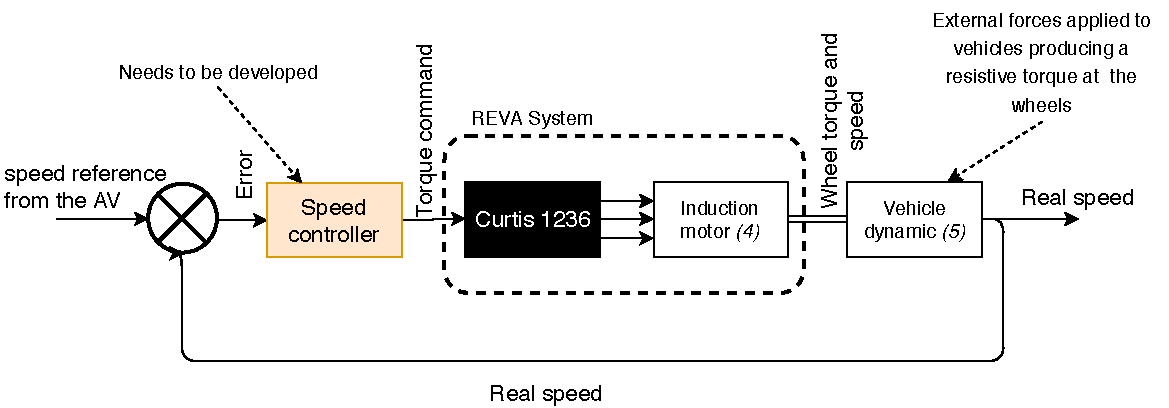
\includegraphics[width=\linewidth]{figure/SystemLoop_2.pdf}
\caption{REVA Control loop}
\label{fig:control_loop_detailed}
\end{figure}

The regulation strategy adopted is to replace the human intervention by a generic \textit{speed controller} while keeping the human regulation principle. This method allows to minimize the modifications on the system and, hence reduces the time and costs investments. Thus, the vehicle system will be kept unchanged, limiting the complexity and possible damage. Indeed, modifying completely or partly the \textit{vehicle} system would imply a lot of work. 

			\subsubsection{System response analysis and open loop-response}
As it has been stated in chapter~\ref{chap:reva}, the battery of the prototyping platform limits the functional possibilities of the vehicle. Thus, before developing a controller, it is required to analyze the REVA's speed response while providing a gas-pedal excitation; which is the aim of this subsection. While having the vehicle on the roller bench, different voltage steps signals were applied to the REVA system. The measurements are illustrated in \textsc{figure}~\ref{fig:step1} and~\ref{fig:step3} for different excitation steps\footnote{As this experiment is not meant generate data for the system identification (see later section), large step responses were chosen because of it operating simplicity and the clear response signal of the vehicle.}. On each figure, the upper graph represents the throttle input, or the voltage at the pedal and the lower part represents the measured vehicle speed. 

From \textsc{figure}~\ref{fig:step1}, it can be concluded that the REVA starts reacting when an approximate voltage signal of 1 V is applied; below this threshold voltage, the vehicle does not react. Additionally, the speed response does not vary while providing a voltage above 3~V. Therefore, the operating region of the REVA within a controller may be designed is (approximately) between 1 and 3 V and around 0 to 35 km/h. Moreover, while the 2 V step signal provides a clean speed response, higher pedal voltage cause an abrupt evolution while reaching the speed of 35~km/h\footnote{Indeed, the Curtis measures a lower battery voltage than expected and limits the maximum output torque and speed at the wheels.}.  

\begin{figure}[hbtp]
\centering
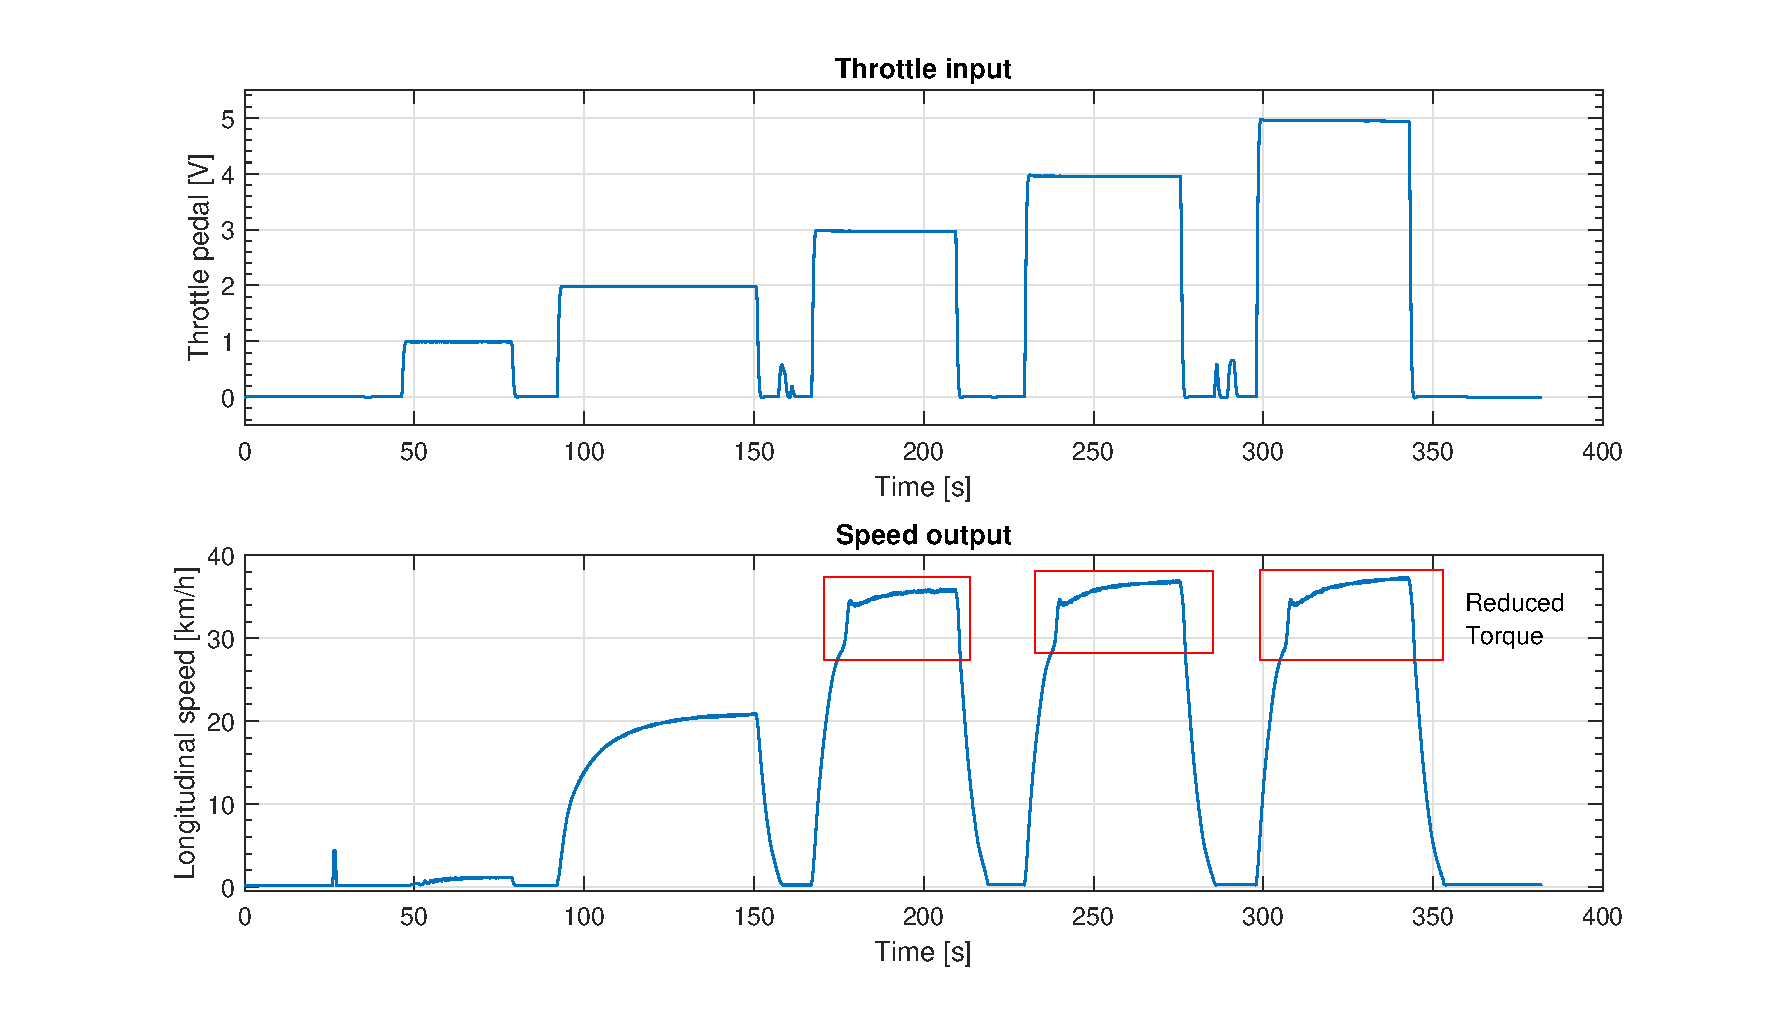
\includegraphics[width=\linewidth]{figure/step_exp1.eps}
\caption{Step responses experiment (minimum resitive torque)}
\label{fig:step1}
\end{figure}

\begin{figure}[hbtp]
\centering
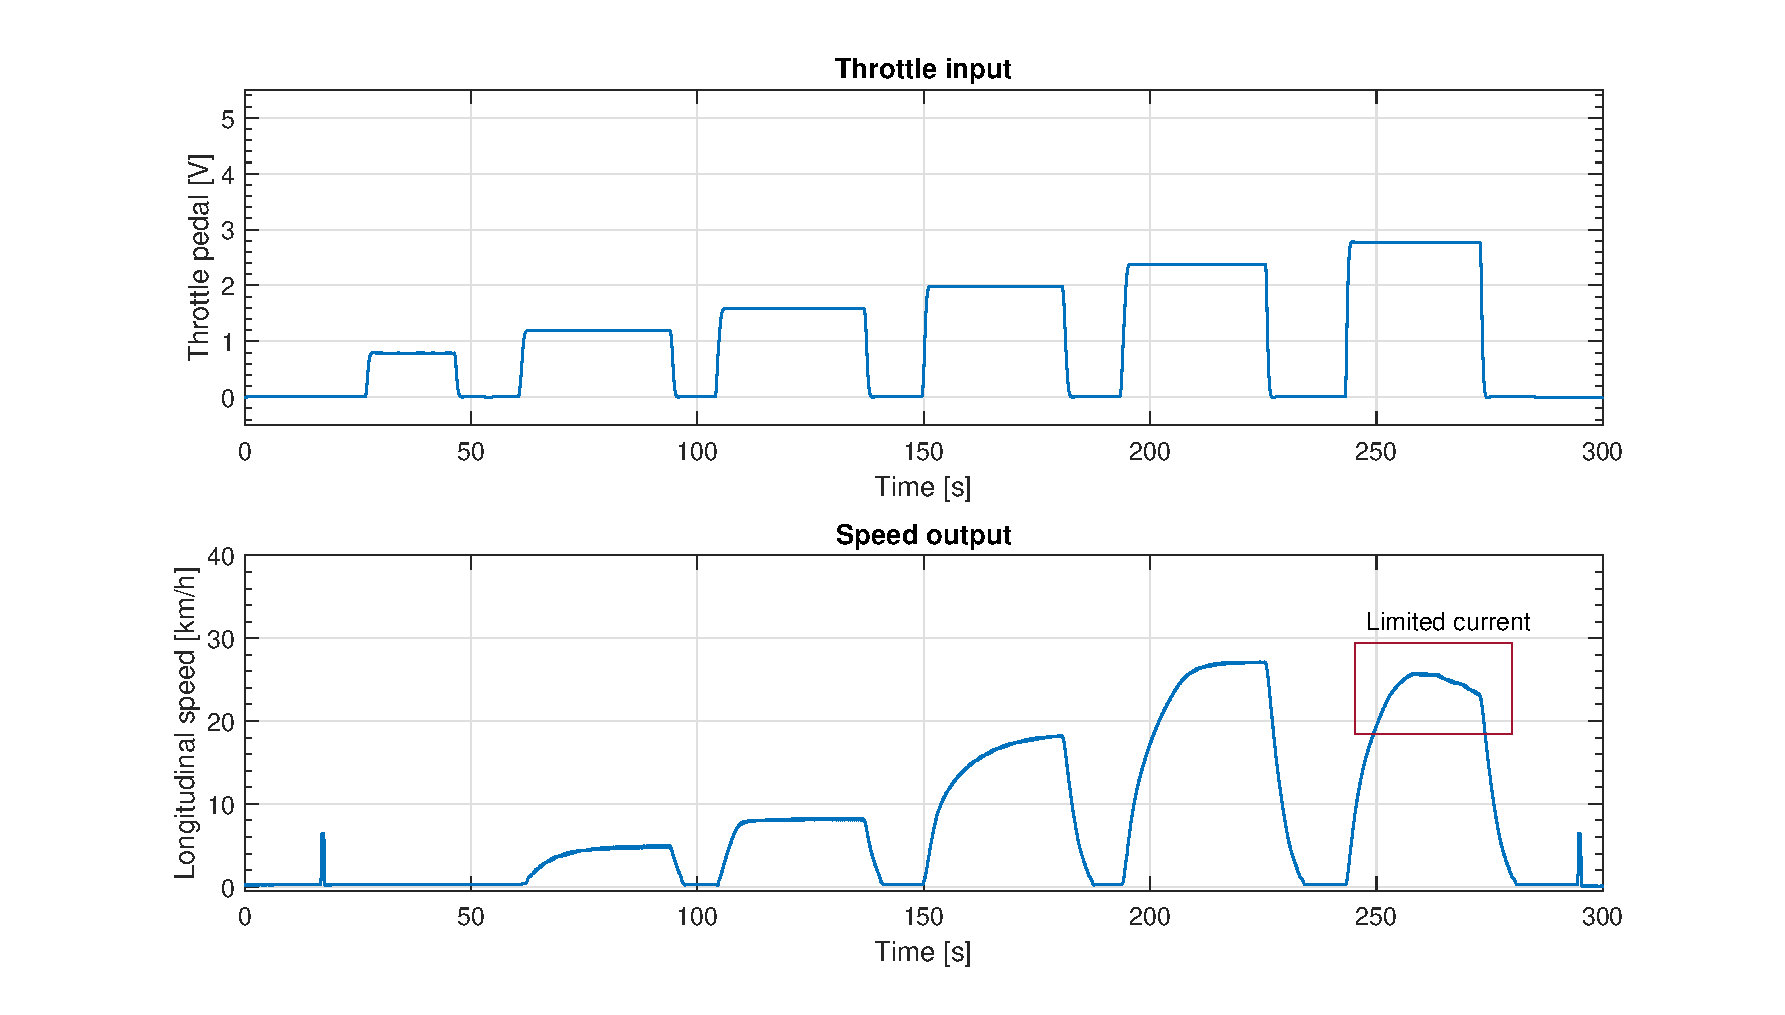
\includegraphics[width=\linewidth]{figure/step_exp2.eps}
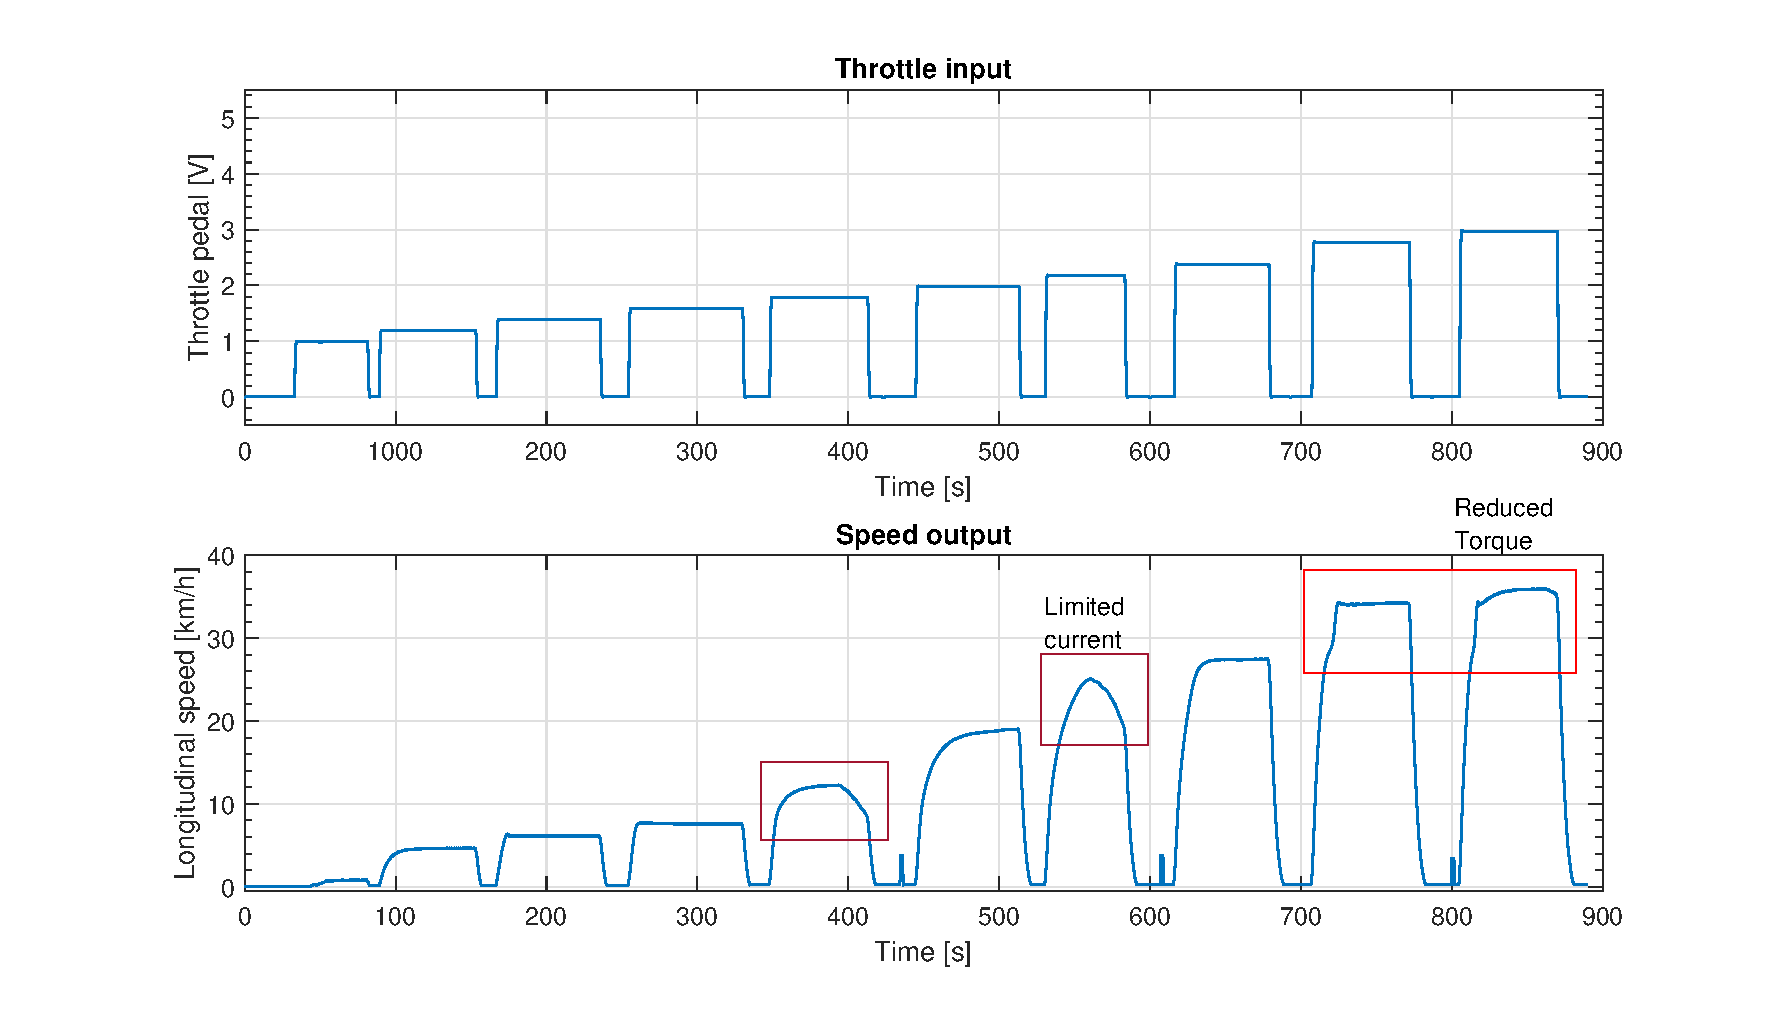
\includegraphics[width=\linewidth]{figure/step_exp3.eps}
\caption{Step responses experiment between 0 and 3~V (minimum resitive torque)}
\label{fig:step3}
\end{figure}

Additional excitation were provided within the operating range of the vehicle are shown in \textsc{figure}~\ref{fig:step3}. This experiment confirms the operating region of the REVA is comprised between 1 to 3 V interval. As the abrupt speed variation happened once again at the same supply voltage, we can conclude this behavior will not affect the torque generation while working in the operating region. However, it can be seen in both experiments that, for some step responses, the vehicle speed drops even if the supply voltage is kept constant. This behavior is due to the motor drive which progressively reduces the current flowing from the batteries to the motor\footnote{Since the voltage provided by the batteries does not comply with expected voltage, the drive switches into a safety mode which reduces the generated torque of the motor until the vehicle stops.}. The problem is most likely due to an uncalibrated \acf{ems} and Curtis 1236 in regard of the used battery set. Even if this trend is understood, it will appear randomly while designing the controller, which may represent a crucial issue. The problem can be easily solved by restarting the vehicle. Nevertheless, a long term solution must be found to achieve an actual speed tracking controller, which implies a large investment in new batteries for a cheap vehicle. In the actual state of the REVA, the challenge is to identify and control a time varying system to track a time varying reference. 

Additionally, the working duration while the vehicle drives correctly has been measured; those results are presented in \textsc{table}~\ref{tab:dead_timing}. At this time, the assumption that the vehicle will be working sufficiently well for an adequate amount of time to build and test the controller is made. 

\begin{table}[hbtp]
\newcolumntype{Y}{>{\centering\arraybackslash}X}
\begin{tabularx}{\textwidth}{ |Y|Y|Y| }
\hline
Pedal Voltage [V] & Speed [km/h] & Mean working time [s] \\
\hline \hline
1,5  & 6 & 300 \\
\hline
2,2  & 24 & 80 \\
\hline
3  & 34 & 60 \\
\hline
\end{tabularx}
\caption{Working duration (until speed drops) at different speed}
\label{tab:dead_timing}
\end{table}

Finally, using multiple steady state speed measures from the previous experiments, the open-loop characteristic of the entire system were plotted in \textsc{figure}~\ref{fig:open-loop}. 

\begin{figure}[hbtp]
\centering
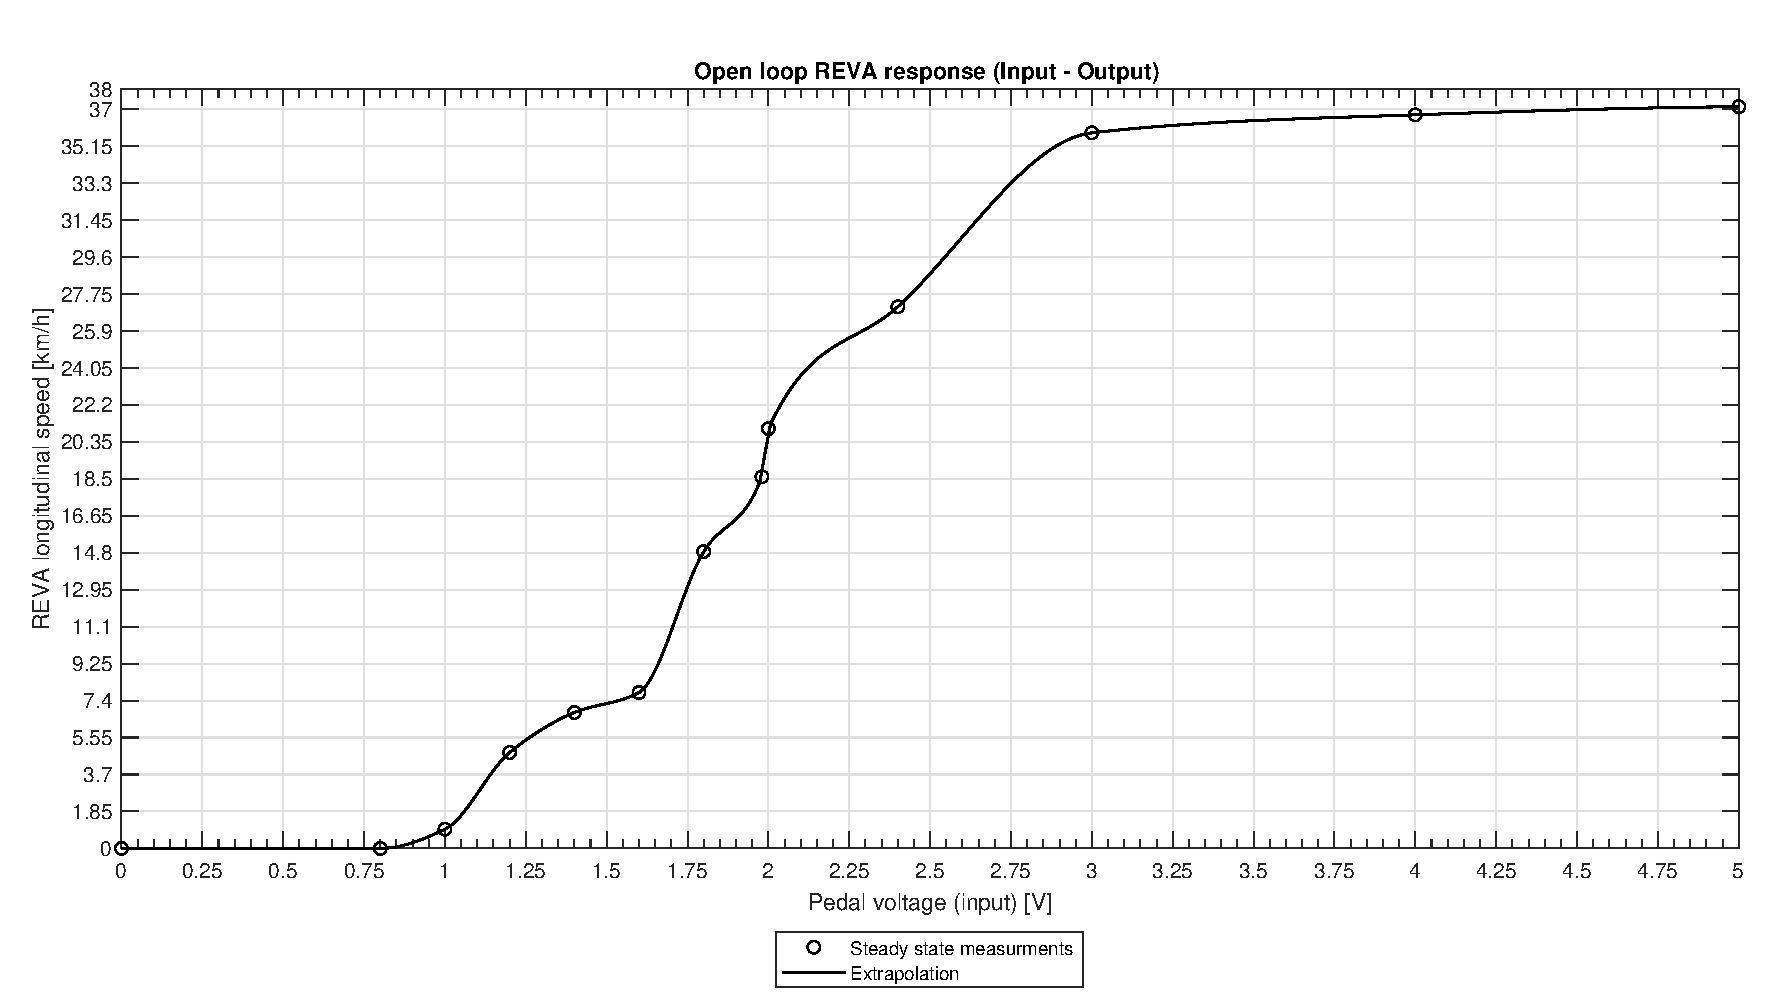
\includegraphics[width=\linewidth]{figure/inout.eps}
\caption{System open loop characteristic (battery low)}
\label{fig:open-loop}
\end{figure}

%\begin{table}[htbp]
\newcolumntype{Y}{>{\centering\arraybackslash}X}
\begin{tabularx}{\textwidth}{ |Y|Y| }
\hline
Input [V] & output [km/h] \\
\hline \hline
$0,00$ & $0,00$ \\
\hline
$0,80$ & $0,00$  \\
\hline
$1,00$ & $0,96$  \\
\hline
$1,2$ & $4,80$  \\
\hline
$1,4$ & $6,80$  \\
\hline
$1,6$ & $7,80$  \\
\hline
$1,8$ & $14,85$  \\
\hline
$1,98$ & $18,60$  \\
\hline
$2,00$ & $21,00$  \\
\hline
$2,4$ & $27,10$  \\
\hline
$3,00$ & $35,80$  \\
\hline
$4,00$ & $36,70$ \\
\hline
$5,00$ & $37,11$ \\
\hline
\end{tabularx}
\caption{Open-loop input-ouput relationship (battery low)}
\end{table}
		\subsection{Modeling}
Until now, the basic strategy for achieving the speed tracking is provided as well as the main requirements of the controlled process. Moreover, the REVA system has been described, and the vehicle behavior has been analyzed. The next step is building an appropriate model of the prototyping vehicle which will be useful for developing the controller. 

Mathematical models of physical systems are key elements to design, analyze and simulate controlled systems~\cite{Modern_Control_System}. Systems dynamic behavior are generally described by ordinary differential equations. Most of them present nonlinear equations which are complex to solve. It is hence a common process to linearize these equations within a certain operating region of the system where the approximated linear description provides acceptable results easier to calculate~\cite{Modern_Control_System}. 

There are two ways of modeling a dynamic system~\cite{sysidLen}: 
\begin{enumerate}
\item The first principle modeling makes use of the laws of physics characterizing the system dynamic. This knowledge is used to build a mathematical model which describes the system behavior. Many equations systems are known and many systems can be described using this method. 
\item Data-driven modeling makes use of data collected from the dynamic system. Whenever the physic behind the system is not characterized by equations, a mathematical model may be build using experimental data from the system; this method is known as System Identification. 
\end{enumerate}

The first principle modeling allows the usage of physical laws from existing literature which may reduce the modeling time (depending of the system complexity). Oppositely, the system identification is not a straight forward technique and requires some expertise and more manipulations; the model structure is guessed in regard of an a priori system knowledge while its parameters are identified using algorithms. While physical equations provide physical meaning to the model parameters, this statement is not true for a model obtained by system identification, which is only a possible way to describe the dynamic. Therefore, the first principle modeling was preferred and primarily investigated in the next paragraph. 
			\subsubsection{First principle modeling}
The REVA system has been divided into multiple subsystems; mainly the induction motor, the Curtis 1236 motor drive, and the vehicle longitudinal dynamic. In order to build the mathematical model of the entire system, each subsystem equation must be developed. Due to complexity of the system, it is likely that non-linearities will happen and will require some attention. 

The induction motor is an electric device which has been largely studied in many literature references. Therefore, its physical equations have been established with more or less complexity depending the assumptions made. Moreover, those models are already available in simulation software such as MATLAB~\cite{chan2011applied}, which reduces the computation time. However, the equations parameters remain unknown and vary from a motor to another. Because of the lack of characteristics provided by the motor manufacturer, those parameters must be found experimentally. Even if the parameters identification process may be time consuming, the experimental process is described in~\cite{abdessemed2011modelisation, giri2013ac}. Once an AC power supply of 28~V capable of supplying up to 350 A is found, the parameter identification might be completed using~\cite{abdessemed2011modelisation, giri2013ac}. Hence, the first principle modeling of the motor can be achieved. 

The Curtis 1236 REVA's motor drive is an \acs{ifoc} that computes the trigger signals applied to the embedded inverter generating the appropriate \acs{ac} voltage and current signals fed to the motor. The \acs{ifoc} torque control method is well known and largely used in the industrial field, thus the general equations are accessible in the literature~\cite{chan2011applied}. However, the different parameters used to achieve this regulation type are not provided by the manufacturer, and, the inverter model is unknown. Moreover, the Curtis doesn't simply generate the signals for the induction motor, it also embeds (unclearly defined) protective and logical systems which are difficult to characterize by equations. Therefore, beside the complexity of this subsystem, its equations are unknown as are the parameters. Hence, the first principle modeling of this system is not achievable without additional information about its behavior. 

Finally, the longitudinal motion equations are given in the literature at different levels of complexity. Many parameters required in those equations are not provided by Mahindra, but some guessing may be achieved using commonly used parameters which can be adjusted during the model validation. Moreover, such models are already implemented in MATLAB which facilitates this subsystem modeling process for simulation.  

This section discussion is summarized in the \textsc{table}~\ref{tab:eqmodelsum}. As stated in this table, the induction motor and longitudinal motion first principle modeling is possible, however the process is not straightforward and will require some time to identify the parameters.  Additionally, the Curtis 1236 knowledge is not sufficient to build an equation based model. Therefore, the system identification method seems more adequate to this subsystem. 

Since applying the system identification is required for at least one of the subsystems, it is less time consuming to apply the method to the entire system and estimate a mathematical model of the REVA power train using measured data. 

\begin{table}[hbtp]
\newcolumntype{Y}{>{\centering\arraybackslash}X}
\begin{tabularx}{\textwidth}{ |Y||Y|Y|Y| }
\hline
 & Induction motor & Curtis 1236 (\acs{ifoc} + inverter + other) &  Longitudinal motion \\
\hline \hline
Equations & Known & Unknown &  Known \\
\hline
Parameters & Experimentally reachable & Provided, but not sufficient & Experimentally reachable \\
\hline 
First principle modeling & Possible & Not possible & Possible \\
\hline 
\end{tabularx}
\caption{First principle modeling summary}
\label{tab:eqmodelsum}
\end{table}


			\subsubsection{Data-driven modeling}
As concluded in the previous subsection, the system identification technique allows to build a model even if the REVA system has a numerous amount of unknowns. System identification is the process of determining the model and its parameters based on experimental data acquired from the system. The general process flowchart to achieve such identification is illustrated in \textsc{figure}~\ref{fig:sysidflowchart}. First, the model structure is chosen based on a priori knowledge about the system dynamic. Next, the experimental phase is designed to collect the necessary data about the system; a chosen input signal is provided to the unknown system and its output response is measured. Those measurements are then processed to create clean and usable data. Using the model structure, the known input and the measured output, the model parameters can be estimated using identification algorithms. Finally, once the model is completed, it is confronted to the real system to verify its reliability. System identification is in general an iterative process where each iteration helps to generate a better estimation of the system~\cite{ControlForUnmandVic}. 

\begin{figure}[hbtp]
\centering
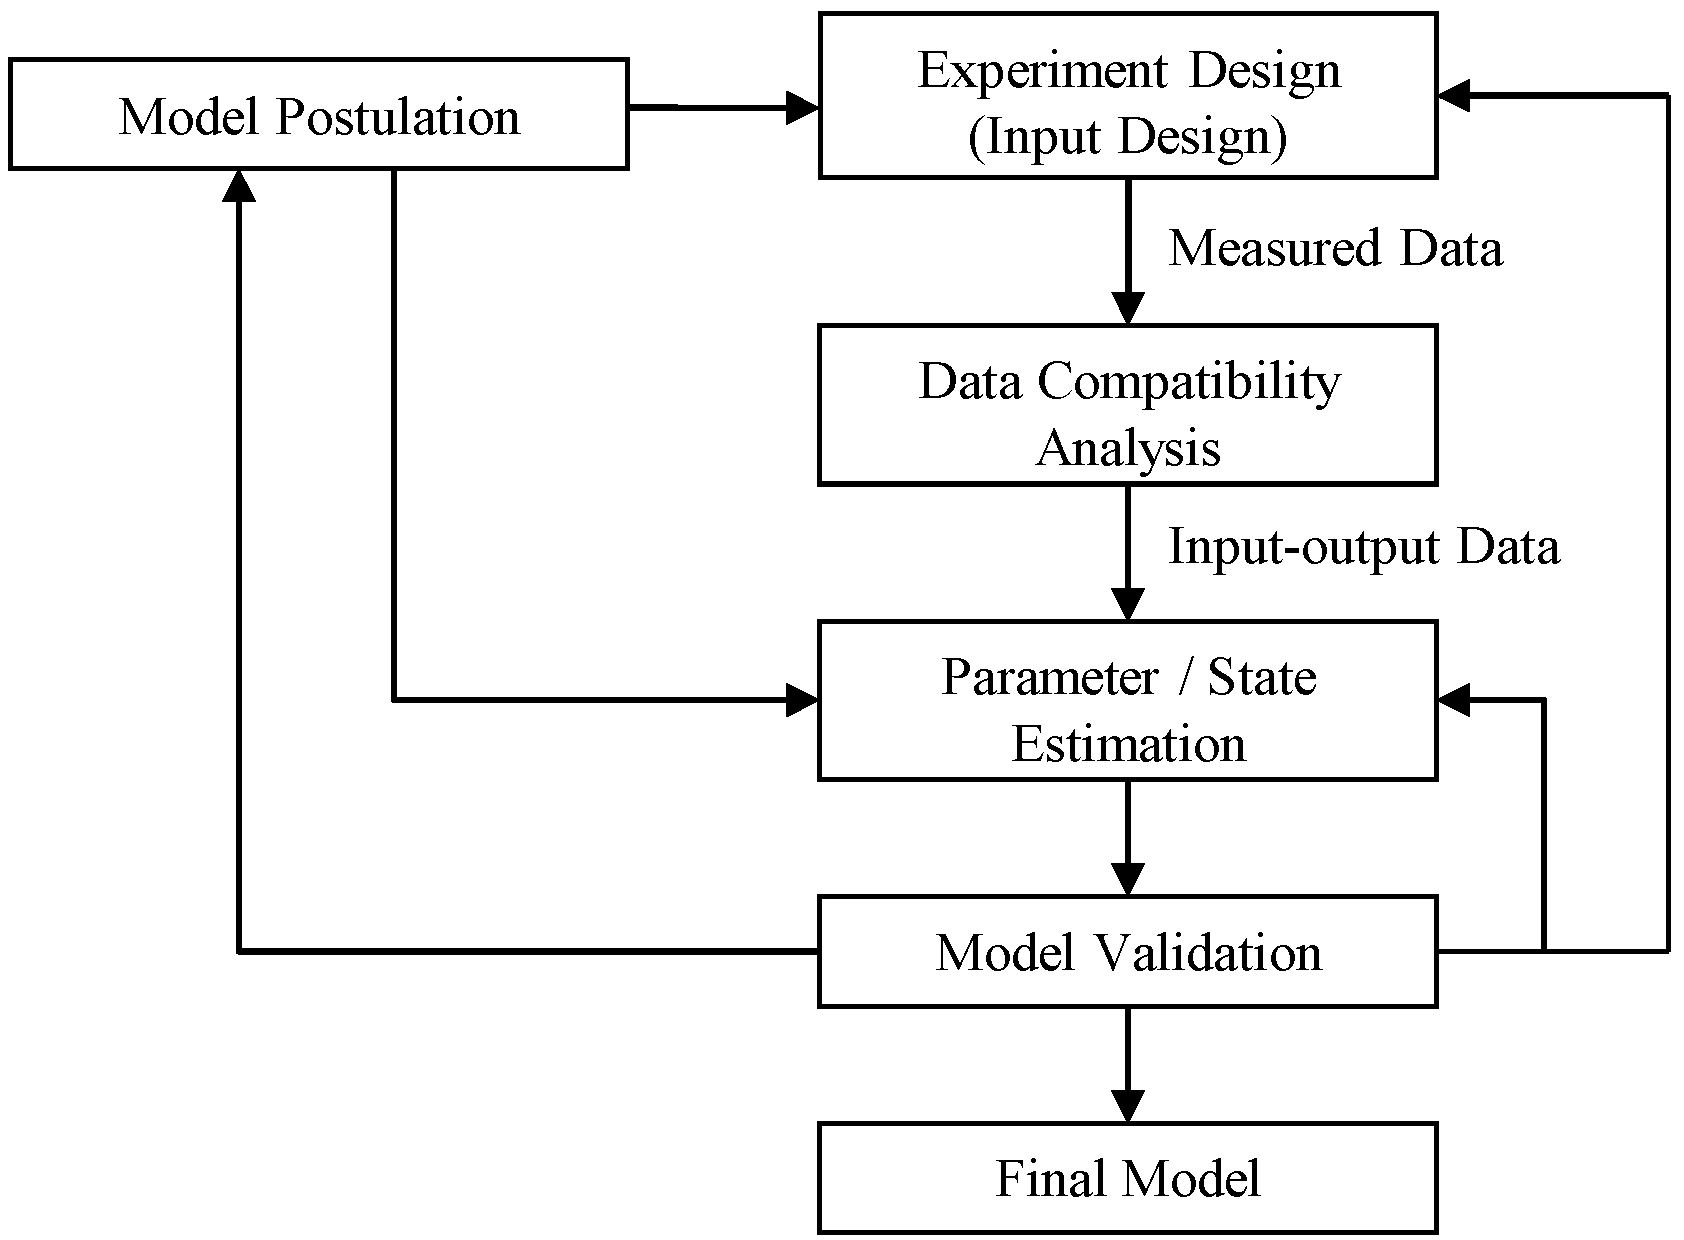
\includegraphics[scale=1.2]{figure/sys_identification_prinicple.png}
\caption{System identification flowchart~\cite{ControlForUnmandVic}}
\label{fig:sysidflowchart}
\end{figure}

In this particular case of system identification applied to the REVA, the experimental phase will be achieved on the roller bench of the \acs{vub}. Indeed, due to its state, the REVA is not suited to be driven on the road safely. The installation limitations make impossible to identify properly the real longitudinal dynamic of the system. Another model structure was therefore chosen to fit the real system at best; the longitudinal dynamic results mostly in a restive torque applied at the wheels shaft, this restive torque varies while driving with multiple factors such as the wind, the inertia, the tire pressure, the road inclination and so on. This resistive torque is thus considered as a perturbation applied to the REVA system and the controller robustness must be sufficient to control the system under any perturbation state. While recording the data of the system, the perturbation will remain constant to avoid affecting the model parameters. The adjusted system which will be estimated by the identification is presented in \textsc{figure}~\ref{fig:SystemAdjustement}. 

\begin{figure}[hbtp]
\centering
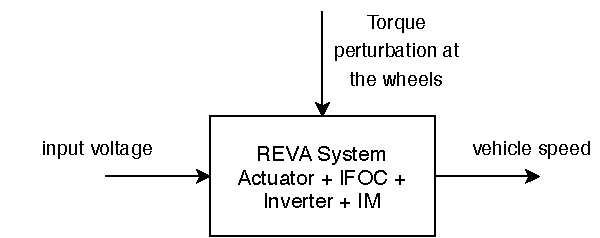
\includegraphics[scale=0.9]{figure/System_adjustement.pdf}
\caption{REVA system adjustment}
\label{fig:SystemAdjustement}
\end{figure}

As shown in \textsc{figure}~\ref{fig:SystemAdjustement}, for a first iteration of data-driven modeling, the system is treated as a SISO system which reduces the difficulty of the identification by removing the brake pedal input. Actually, automotive speed control generally separates the acceleration and the deceleration regulation using finite state machines principle~\cite{DAS_handbook}. Therefore, two models of the system should be developed; one for the throttle actuation and one for the brake actuation. Each state (mainly acceleration, deceleration and stand-by) is activated while a transition is activated.  Using the state machine principle eases the identification by reducing the system complexity but requires 2 identifications for each actuation. In this document, only the throttle actuation for speed tracking will be investigated. 

From previous data analysis of the REVA, its response to a step input of $0,25$~V is a curve similar to a first order system. The system complexity and composition of multiple devices surely introduces nonlinear operating regions\footnote{Since the system comprises an \acs{ifoc} which already regulates the torque at the wheels, it is not surprising to obtain such first order curve even if the system complexity is high.}. Therefore, if a linear first order model is to be used, it is required to linearize the real system. To do so, only small excitation signals will be provided to the real system to generate the output data. For each excitation, because of the reduced operating region where the system is excited, it is possible to assume that the system is linear, and its approximated model will be as well within this operating region. Other system model are commonly used and might fit the case study as well, however, the simplicity of a first order model for the REVA is appreciable and eases later controller development. 

First order model transfer function in the Laplace domain is provided in \textsc{equation}~\ref{eq:first_order}, where $K$ is the gain, $\tau$ is the time constant, $T$ is time delay, $Y(s)$ is the output signal (or the speed) and $X(s)$ is the input signal (or the pedal voltage). $K$, $\tau$ and $T$ are the parameters that will be estimated through the system identification process (as shown with arbitrary numbers in the last equation of the equality). Indeed, measuring $Y$, knowing $X$ the provided signal, and the model structure, the parameters are recognizable. 

\begin{equation}
G(s)  = \dfrac{Y(s)}{X(s)} = \dfrac{K}{\tau \: s + 1} \: e^{T \:s}  = \dfrac{6,8}{4,2\: s + 1} \: e^{0,205\:s}
\label{eq:first_order}
\end{equation}

			\subsubsection{Exciting signals}
The experimental design of system identification requires selecting an input signal. This signal stimulates the process and its response is measured; the more the excitation is appropriate the more the response is relevant for identification. Among a multitude of excitation signals for linear black-box\footnote{Synonym for system identification} modeling, three famous are shortly described here and the most suited is selected~\cite{researchgate,tangirala_2013}.

The step signal is the most popular method in the industry because of its design and generation easiness. However, it requires a long excitation time up to steady states, and because a step is provided in open-loop process, the measure is sensitive to disturbances. Finally, this signal is only suited for linear system modeling. 

The \acf{prbs} is a binary sequence generated by a deterministic algorithm nonetheless difficult to predict. Its randomness and its periodic nature result generally in a more accurate estimation making this method famous for linear system modeling. However, it is applied to an open-loop process and the measures are as well sensitive to disturbances. 

While a step signal does not capture any frequency response of the system, \acs{prbs} does capture a bit due to its periodic variation. The frequency information is generally appreciated while identifying a system. Thus, a chirp signal (or sinus with constantly increasing frequency) is also commonly fed to the open-loop process for modeling. Oppositely to step and \acs{prbs} excitation that provides a time-domain characteristic, the chirp method permits a frequency response analysis of the system. Nonetheless, chirp excitation requires a longer excitation time than the others.  

While each of those signals are possible candidates to approximate linear models of the REVA, the step signal method was preferred in a first iteration because of its application easiness. Actually, it was difficult to find a general recipe to build an appropriate \acs{prbs} signal (amplitude, frequency, algorithms and etc.). Finally, since the chirp signal requires a longer excitation time, the vehicle may end up in the none-working (\textsc{table}~\ref{tab:dead_timing}) condition making the experiment irrelevant. 

To linearize the system within an operating region, the amplitude of the input step signal is commonly chosen to cause a $3$ to $10$~\% response amplitude of the total operating range. \textsc{Figure}~\ref{fig:open-loop} speed axis is divided in such a way that each interval represent 5\% of the total Y-axis magnitude. The input voltage amplitude can be read using the extrapolation curve. For example, to identify a linear system within the 0 to 1,85~km/h range, the process is firstly fed with an input voltage of 0,75~V until it reaches steady state, then an incremental step of 0,35~V is applied to the system which produces the useful data for the identification. 

			\subsubsection{Data treatment and analysis}
The purpose of examining the data collected from the experiment is selecting and preprocessing the measurements to build a suitable dataset for the identification. Since the quality of this dataset affects the reliability of the identified system, this treatment and analysis phase is important and includes the methods described below. 

The visual inspection is the best way to find major corruption with the data collection as abnormal measurements (outliers), noise perturbation, etc. Besides, it provides a general statement of the data, and allows the user to predict and select the usable data ranges  as well as the preprocessing actions. 

In this experiment, the principle is to identify multiple linearized versions of the true system around multiple operating points. For each operating range where an experimental identification is led, it is necessary to subtract the operating points value from the
raw data samples because linearization is done with respect to the signal
values relative to this operating point. This phase is called offset removing of the signal. 

In general the acquired signal is subject to external process perturbation which are seen in the measurement as trends and outliers in the signal. Those must be identified and removed so it does not influence the identification. 

Finally, the measurement is inherently influenced by other measurement devices and their electromagnetic fields produce high frequency noises in the measures which must be filtered. 
			\subsubsection{Useful software}
The system identification process requires applying complicated algorithms which have not been  presented in this document. Those algorithms are already integrated in famous softwares, which eases the execution of this procedure. The System Identification Toolbox proposed by Lennart Ljung provides a complete MATLAB toolbox for running such process. LabVIEW System Identification toolkit from \acf{ni} provides similarly LabVIEW functions to achieve this as well. The major advantage of the MATLAB tool is its convenient graphical user interface which I have found intuitive. Both tools have a well made beginner user guide However, even if both toolboxes seem equivalent, from a previous experience with LabVIEW, MATLAB user interface is a strong asset, and was hence preferred. 

DIAdem is a software proposed by National Instruments for managing and analyzing large amount of collected data. At the beginning, the software may be difficult to handle, but is after all a powerful tool which facilitates the visual inspection and the filtering of the REVA measurements.
			
			\subsubsection*{Workflow summary}
\begin{figure}[H]
\centering
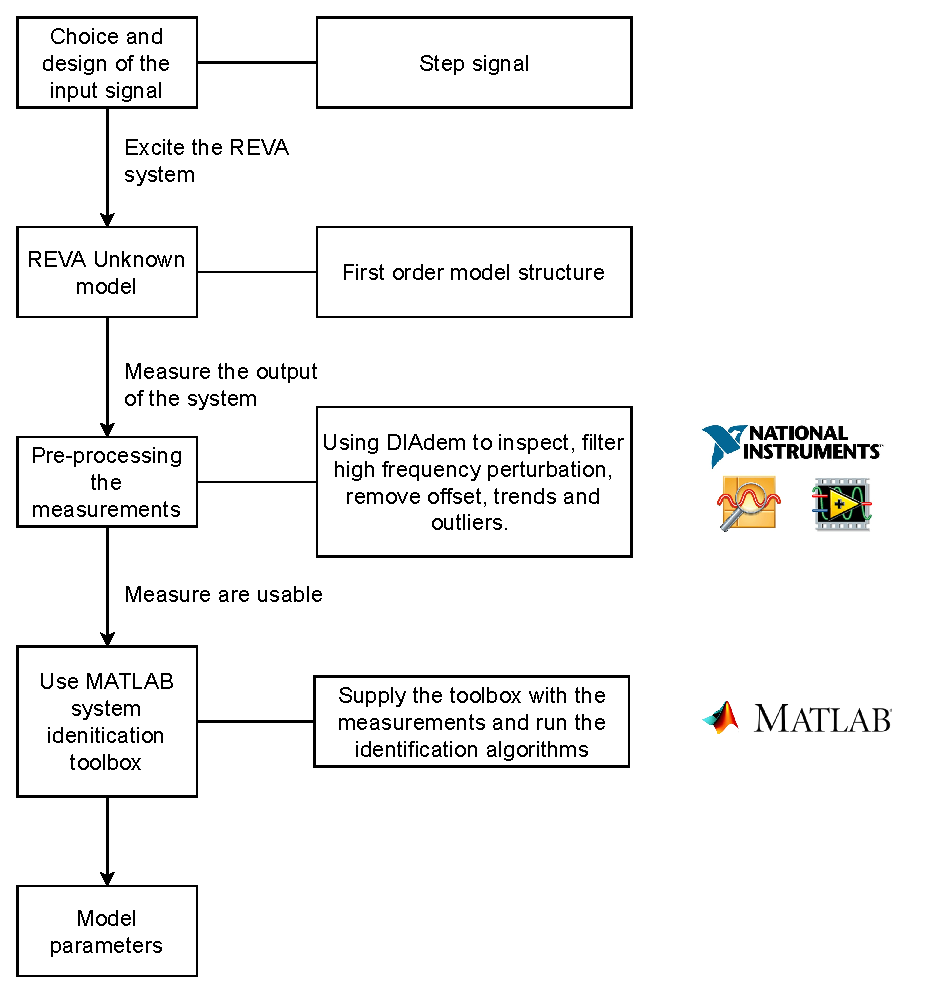
\includegraphics[scale=0.7]{figure/SysIDworkdlow.eps}
\caption{System identification workflow}
\end{figure}

		\subsection{Controller choice}
In the previous section was introduced the system identification technique which would provide linear mathematical models of the REVA. This model is useful to build a controller which would achieve the regulation and bring the interesting possibility of simulating the controlled system built. This section aim is to delve the controller type selection and later its parameter identification. 

The difference between the desired and the actual output is equal to the error. This value is given as an input to the controller which computes the command signal then provides it to the actuator in order to regulate the process, and hence, reducing this error. The controller is therefore the heart of the regulation; its choice and design is a milestone to compute appropriate command signals and thus achieve the regulation to meet the tender specification. In the literature, multiple controllers have been proposed for vehicles longitudinal speed control\footnote{Those were inspired from \acs{adas} cruise control and adaptive cruise control.}; mainly \acf{pid}, \acf{mpc} and Fuzzy controllers~\cite{eskandarian2012handbook}. \acf{nn} controller has lately gain an interest as well.  Some of those controller types have been studied, and are shortly described below, then the most suited control method has been chosen. \cite{Astrom_Murray}

\acf{pid} is by far the most famous controller in the industry because of its simplicity, and easiness to develop. Generally most industrial processes are reasonably well controlled by \acs{pid} provided that the performance requirements are not too high. Such controller block diagram is provided in \textsc{figure}~\ref{fig:pidblock}. The output control signal $u$ is entirely formed based on the error $e$ following the input/output relationship given by equation~\ref{eq:pid}. As shown, the controller action relies on the sum of 3 terms; the proportional gain $k_p$, the integral gain $k_i$, and the derivative gain $k_d$. Each term has its own effect on the regulated system. Increasing the proportional gain decreases the steady state error of the system but increases its oscillatory mode as well. The integrator term ensures that the error ends up to zero if the system reaches steady states. Increasing $k_i$ makes the system respond faster but also increases its transient oscillatory mode. The derivative term brings a predictive action and increasing this term provides a more damped system response. However, a too high $k_d$ deteriorates the controller performances. Each parameter modification has benefits and drawbacks; the art of selecting these parameters to obtain the excepted regulated system is known as parameter tuning and mostly a story of compromises~\cite{Astrom_Murray}. 

\begin{equation}
u = k_p e + k_i \int_0^t{e(\tau) \mathrm{d}\tau} + k_d \dfrac{\mathrm{d}e}{\mathrm{d}t} = k_p e + \dfrac{1}{T_i} \int_0^t{e(\tau) \mathrm{d}\tau} + T_d \dfrac{\mathrm{d}e}{\mathrm{d}t}
\label{eq:pid}
\end{equation}

\begin{figure}[hbtp]
\centering
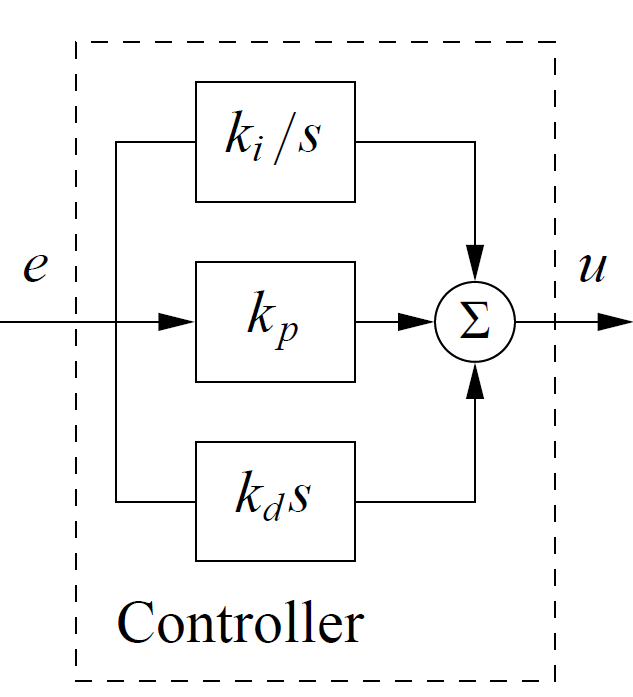
\includegraphics[scale=0.28]{figure/pid_block.png}
\caption{PID block diagram~\cite{Astrom_Murray}}
\label{fig:pidblock}
\end{figure}

As a general statement, the more complicated is the system dynamic the more complicated will be the controller to effectively achieve the regulation. When the system dynamic is essentially of the first order, it has been shown that the derivative action of the \acs{pid} does not improve the regulation. Therefore, since the selected model of the REVA is of the first order, a simple \acs{pi} controller design is considered. Despite the given benefits of using \acs{pid} controllers, those are not suited to control nonlinear process (such as the REVA) within their entire operating range~\cite{PID_theory_control_tuning}. Therefore, depending on the system and the control requirements, more advanced method control exists; \acs{mpc}, adaptive control, Fuzzy, and \acs{nn} control.

\acf{mpc} is an advanced control technique mostly used for complex regulation problems. Having a reasonably accurate model of the system dynamic, this model and the current measurements can be used to predict the upcoming response of the system. Based on predictions and measurements, the required change in input can be calculated to satisfy the regulation of the process. The reliability of such model-based approach depends on the quality of the model. 

In order to regulate systems with time or operating region varying characteristics such as the REVA, adaptive control techniques have been developed. An adaptive technique is a control method where the controller parameters are continuously adjusted to accommodate the changes in system dynamics. \textsc{Figure}~\ref{fig:adaptiveGuide} guides the choice among the different techniques. In this present case study, the REVA system dynamic varies and thus constant parameter controller is not suited. However, the variation of dynamic remains predictable (while the vehicle operates correctly), therefore (from \textsc{figure}~\ref{fig:adaptiveGuide}), the gain scheduling technique is an appropriate candidate. Gain scheduling is the simplest form of adaptive control and has proven to be effective in operating region varying process regulation. A finite set of controller parameters are stored in a table, while the process is running, one (or more) scheduling variable is observed. Such variable correlates the changes in process dynamic, thus, depending on the scheduling variable state, a different set of parameters is selected from the table and provided to the controller. Since the scheduling variable reflects the dynamic changes and is responsible of the parameter selection, the controller is adjusted with regard to the system dynamic~\cite{PID_theory_control_tuning}. Gain scheduling is widely used with \acs{pid} controller where each proportional, integral and derivative parameters varies depending on the operating region. In this case of speed regulation, the "simplicity" of both \acs{pi} and gain scheduling are appreciated. In \textsc{figure}~\ref{fig:GainSchedulingLoop}, a controlled loop is proposed for this case study, where the vehicle speed and the external torque are used as gain scheduling variables. 

\begin{figure}[hbtp]
\centering
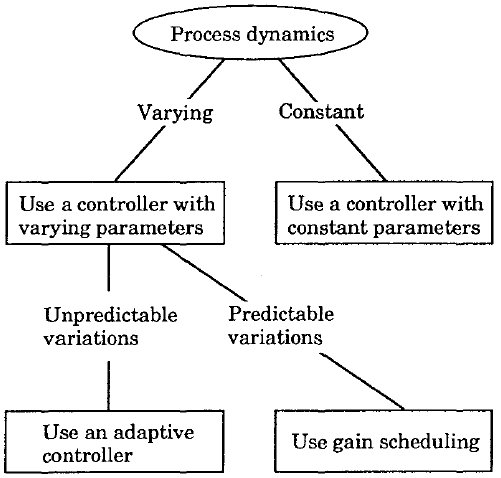
\includegraphics[scale=0.6]{figure/adaptiveGuide.png}
\caption{When to use different adaptive technique~\cite{PID_theory_control_tuning}}
\label{fig:adaptiveGuide}
\end{figure}

\begin{figure}[hbtp]
\centering
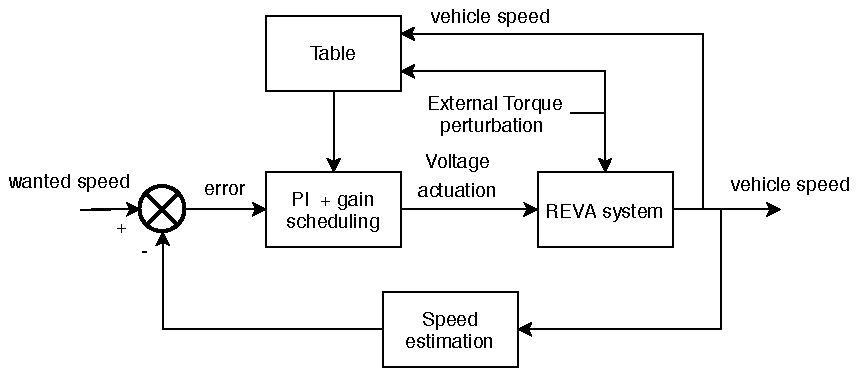
\includegraphics[scale=1]{figure/RegulationLoop.pdf}
\caption{Control loop using gain scheduling}
\label{fig:GainSchedulingLoop}
\end{figure}    

\begin{table}[hbtp]
\newcolumntype{Y}{>{\centering\arraybackslash}X}
\begin{tabularx}{\textwidth}{ Y||Y|Y|Y|Y|Y }
\hline
 & PI & PI + Gain scheduling & \acs{mpc} & Fuzzy control & \acs{nn} control\\
 \hline \hline \hline
Nonlinear control & No & Yes & Yes & Yes & Yes \\
\hline 
Model quality control effect & Low & Low & High & Low & Low \\
\hline
Computation time & Shortest & Short & Longest & Shorter & Shorter \\
\hline
Stability and performance analysis tools & Yes & Yes (may be difficult) & Yes (may be difficult) & No & No \\
\hline
Controller parameter & 2 & $2 \: \times$ number of PI & ? & Many & Many \\
\hline
Deployment easiness (labVIEW) & Existing module & Existing modules & Existing module & Existing module & No modules \\
\hline \hline
Final preference & $\times$ & \checkmark\checkmark\checkmark & $\times$ & \checkmark\checkmark & \checkmark \\
\hline
\end{tabularx}
\caption{Comparison of system controller candidate}
\label{tab:ControllerCompa}
\end{table}

To conclude this section, a comparison of the different controllers is proposed in \textsc{table}~\ref{tab:ControllerCompa}. This table was build according to my personal interpretation of the different consulted documents focusing on speed control achievement. Therefore it may not be applicable to every project. The most appropriate choices in this case, are the \acs{pi} with gain scheduling and the Fuzzy controller. Both of them should be able to control the nonlinear REVA system, and have an integrated module within LabVIEW\footnote{As it will be explained in the next section, LabVIEW software will be used to build the regulation loop.} which eases the development process. Even if the linguistic control based laws of the fuzzy controller is appealing, its difficulty to assess stability and performance is its weakness. Oppositely, the PI with gain scheduling method allows to proceed those valuable analysis (for each parameter set within its operating region) making this candidate the favorite choice.  For this reasons, the regulation loop proposed in \textsc{figure}~\ref{fig:GainSchedulingLoop} was adopted. 

		\subsection*{Short summary}
\begin{figure}[H]
\centering
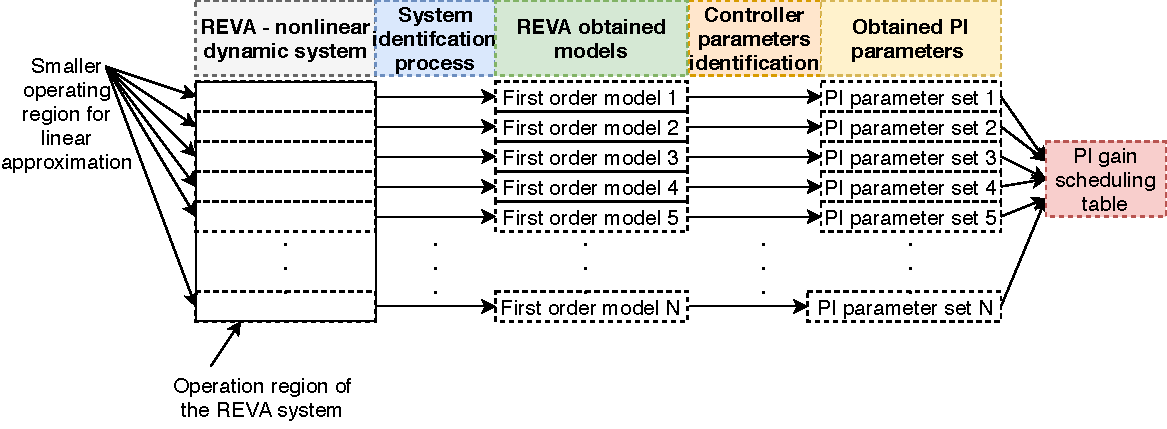
\includegraphics[width=\linewidth]{figure/SysID.pdf}
\caption{System identification process and \acs{pi} parameter estimation workflow}
\end{figure}


	\section{Implementation}
Until now, a theoretical research has been led which results into a procedure and software tools proposal to find the system model and the controller parameter required to construct the speed regulation loop. The current section presents the practical work made to apply those theoretical approaches to this REVA case study which involves hardware and software parallel developments. The proposition will therefore ensure the system identification\footnote{which will be used to find \acs{pi} $k$, $k_i$ parameter}, and the process control itself. For purpose of reducing costs and development time, the available material in the lab has been used. Moreover, a previous student has improved the existing roller bench set-up of the \acs{vub} by creating (and/or updating) the roller software and hardware, a notable work which have been used in this implementation. 

Part of his contribution was to allow an operator to drive standard speed cycles\footnote{Speed cyle : }. However, following the speed cycle reference has shown to be difficult due to small tolerance within which the real vehicle speed must remain to validate the experiment. Integrating a speed control (that automatically follow the standard speed cycle) into the updated roller bench would ease speed cycle experiments. Therefore, at this time the speed control project has two objectives: 

\begin{itemize}
\item[--] Build a speed controller feature for an automated REVA 
\item[--] Use this speed controller to easily achieve REVA driving cycle. In other words, this could be seen as the proof of concept of the speed controller. 
\end{itemize}

The REVA speed controller creation is consequently an extension of the effort made by the previous student to improve the roller bench performances. And, as a continuity matter, his software and hardware decisions were considered and adopted while building the REVA speed control development. 

As stated in the student's master thesis~\cite{RollerBenchThesis}, the software hosting device choice has been made in favor of the National Instrument \acf{crio} which allows multiple computation tasks. The CompactRIO is a rugged, reconfigurable embedded system containing three components; a \acf{rt} controller, a reconfigurable field-programmable gate array (FPGA), and industrial Input/Output modules~\cite{national_instrument_2009}. 

The deterministic nature brought by the real-time controller of such device and the built-in safety optimized OS were indeed fulfilling the roller bench improvement criteria. Additionally, its availability in the laboratory has made this software hosting device a strong candidate. Even if the roller bench improvement and speed control requirements are different, the CompactRIO capabilities enable the speed tracking development. However, the choice of using the cRIO for speed control purpose would not allow to embed the solution within the REVA (external power supply, speed measure made externally of the car). Nevertheless, other devices were not available and the cRIO would still allow to build the proof of concept experiment. Moreover, it was not easy to access to wheel speed measure directly from the car, and it was easier, as first experimentation, to estimate the vehicle velocity from the bench. Nonetheless, as a future work, it will be mandatory to design an embedded software and hardware architecture for hosting automated features, a task considered out of scope of this thesis. 

Following the \acs{crio} device selection, it was mandatory to use the LabVIEW National Instrument. LabVIEW is a system-design platform and development environment for a visual programming language~\cite{Labview_wiki}. Instead of writing specific code lines, this programming environment uses block diagrams connected together in order to achieve specific tasks. It allows comprehensive coding  and eases the programming process thanks to its graphical nature. Even if this programming language is heavily used in process industries, it is not recognized as a standard for automotive systems, where low level language (such as variant of C and C\#, UML, etc.) are preferred for performance and reliability reasons. Nevertheless, LabVIEW capabilities have been proven, and it is perfectly able to achieve the intended work of this master thesis. Although, as a future work along the design of an embedded system architecture, another programming language may be considered to achieve automated features. Both hardware and software considerations are summarized in~\textsc{table}~\ref{tab:SoftHardSum}. 

\begin{table}[hbtp]
\newcolumntype{Y}{>{\centering\arraybackslash}X}
\begin{tabularx}{\textwidth}{ |Y|Y|Y| }
\hline
LabVIEW & Acceptable to design the speed control & Is the fastest way to provide a tangible result \\
\hline 
CompactRIO & Acceptable for achieving the measurement and actuate the vehicle & Only available input/output device in the laboratory\\
\hline
\end{tabularx}
\caption{Software and hardware decision summary}
\label{tab:SoftHardSum}
\end{table}

Additionally to the LabVIEW and \acs{crio} combination, MATLAB, and DIAdem softwares have also been used. DIAdem is easy and powerful to process the collected data while MATLAB is a powerful software providing controller design and system identification toolboxes. Even if LabVIEW also provides means to achieve those tasks, MATLAB toolbox has a comfortable graphical interface which eases its usage even for newbie users. Therefore, the regulation loop has been implemented in LabVIEW as well as the system identification experiment (input design, and data collection) while the model and controller parameters identification are achieved offline using both DIAdem and MATLAB. Even if LabVIEW is described as a straightforward programming language, in practice, it has been difficult to find and arrange the blocks from the wealth of possibilities to achieve simple tasks. 

			\subsection{CompactRIO principle}
The National Instruments \acs{crio}  is a modular device which is split up into 3 distinct parts; the \acf{rt} controller, the chassis which ensures the \acs{fpga}, and the input/output modules allowing the communication with the external environment. Moreover, there is clear division between the cRIO and the host computer;  the host runs LabVIEW (as well as the appropriate NI real-time and NI FPGA software), where a control or monitoring User Interface can be developed and the \acs{crio} \acs{rt} and \acs{fpga} can be programmed as wished. The host and its attached \acs{crio} are linked by an Ethernet cable, resulting in the architecture shown in \textsc{figure}~\ref{fig:cRIOPrinicple}. \acs{crio} modules share data with each other via different communication mechanism proposed by National Instruments which are not described here and the host communicates with the \acs{crio} as well using different methods which are neither described. Ensuring effective communication between host and modules might be fastidious and is out of scope for this thesis which will use predefined algorithms. 

In this case study, the REVA system dynamic is slow and doesn't require the \acs{rt} controller deterministic capabilities and the regulation loop can be realized using classical LabVIEW programming on the host computer. Also, the \acs{rt} library is limited and would increase the amount of work to implement both the control regulation and the system identification using the \acs{rt} modules; therefore it will not be utilized in this case. The \acs{fpga} chassis is however of a great interest; its fast computation capabilities will be used to achieve online data processing from the roller bench measurement. From LabVIEW it is possible to control the input and output modules connected on the \acs{fpga} chassis. For this reason, the FPGA will play the junction role between the software (LabVIEW on host computer) and the installation (REVA and roller bench). 
\begin{figure}[hbtp]
\centering
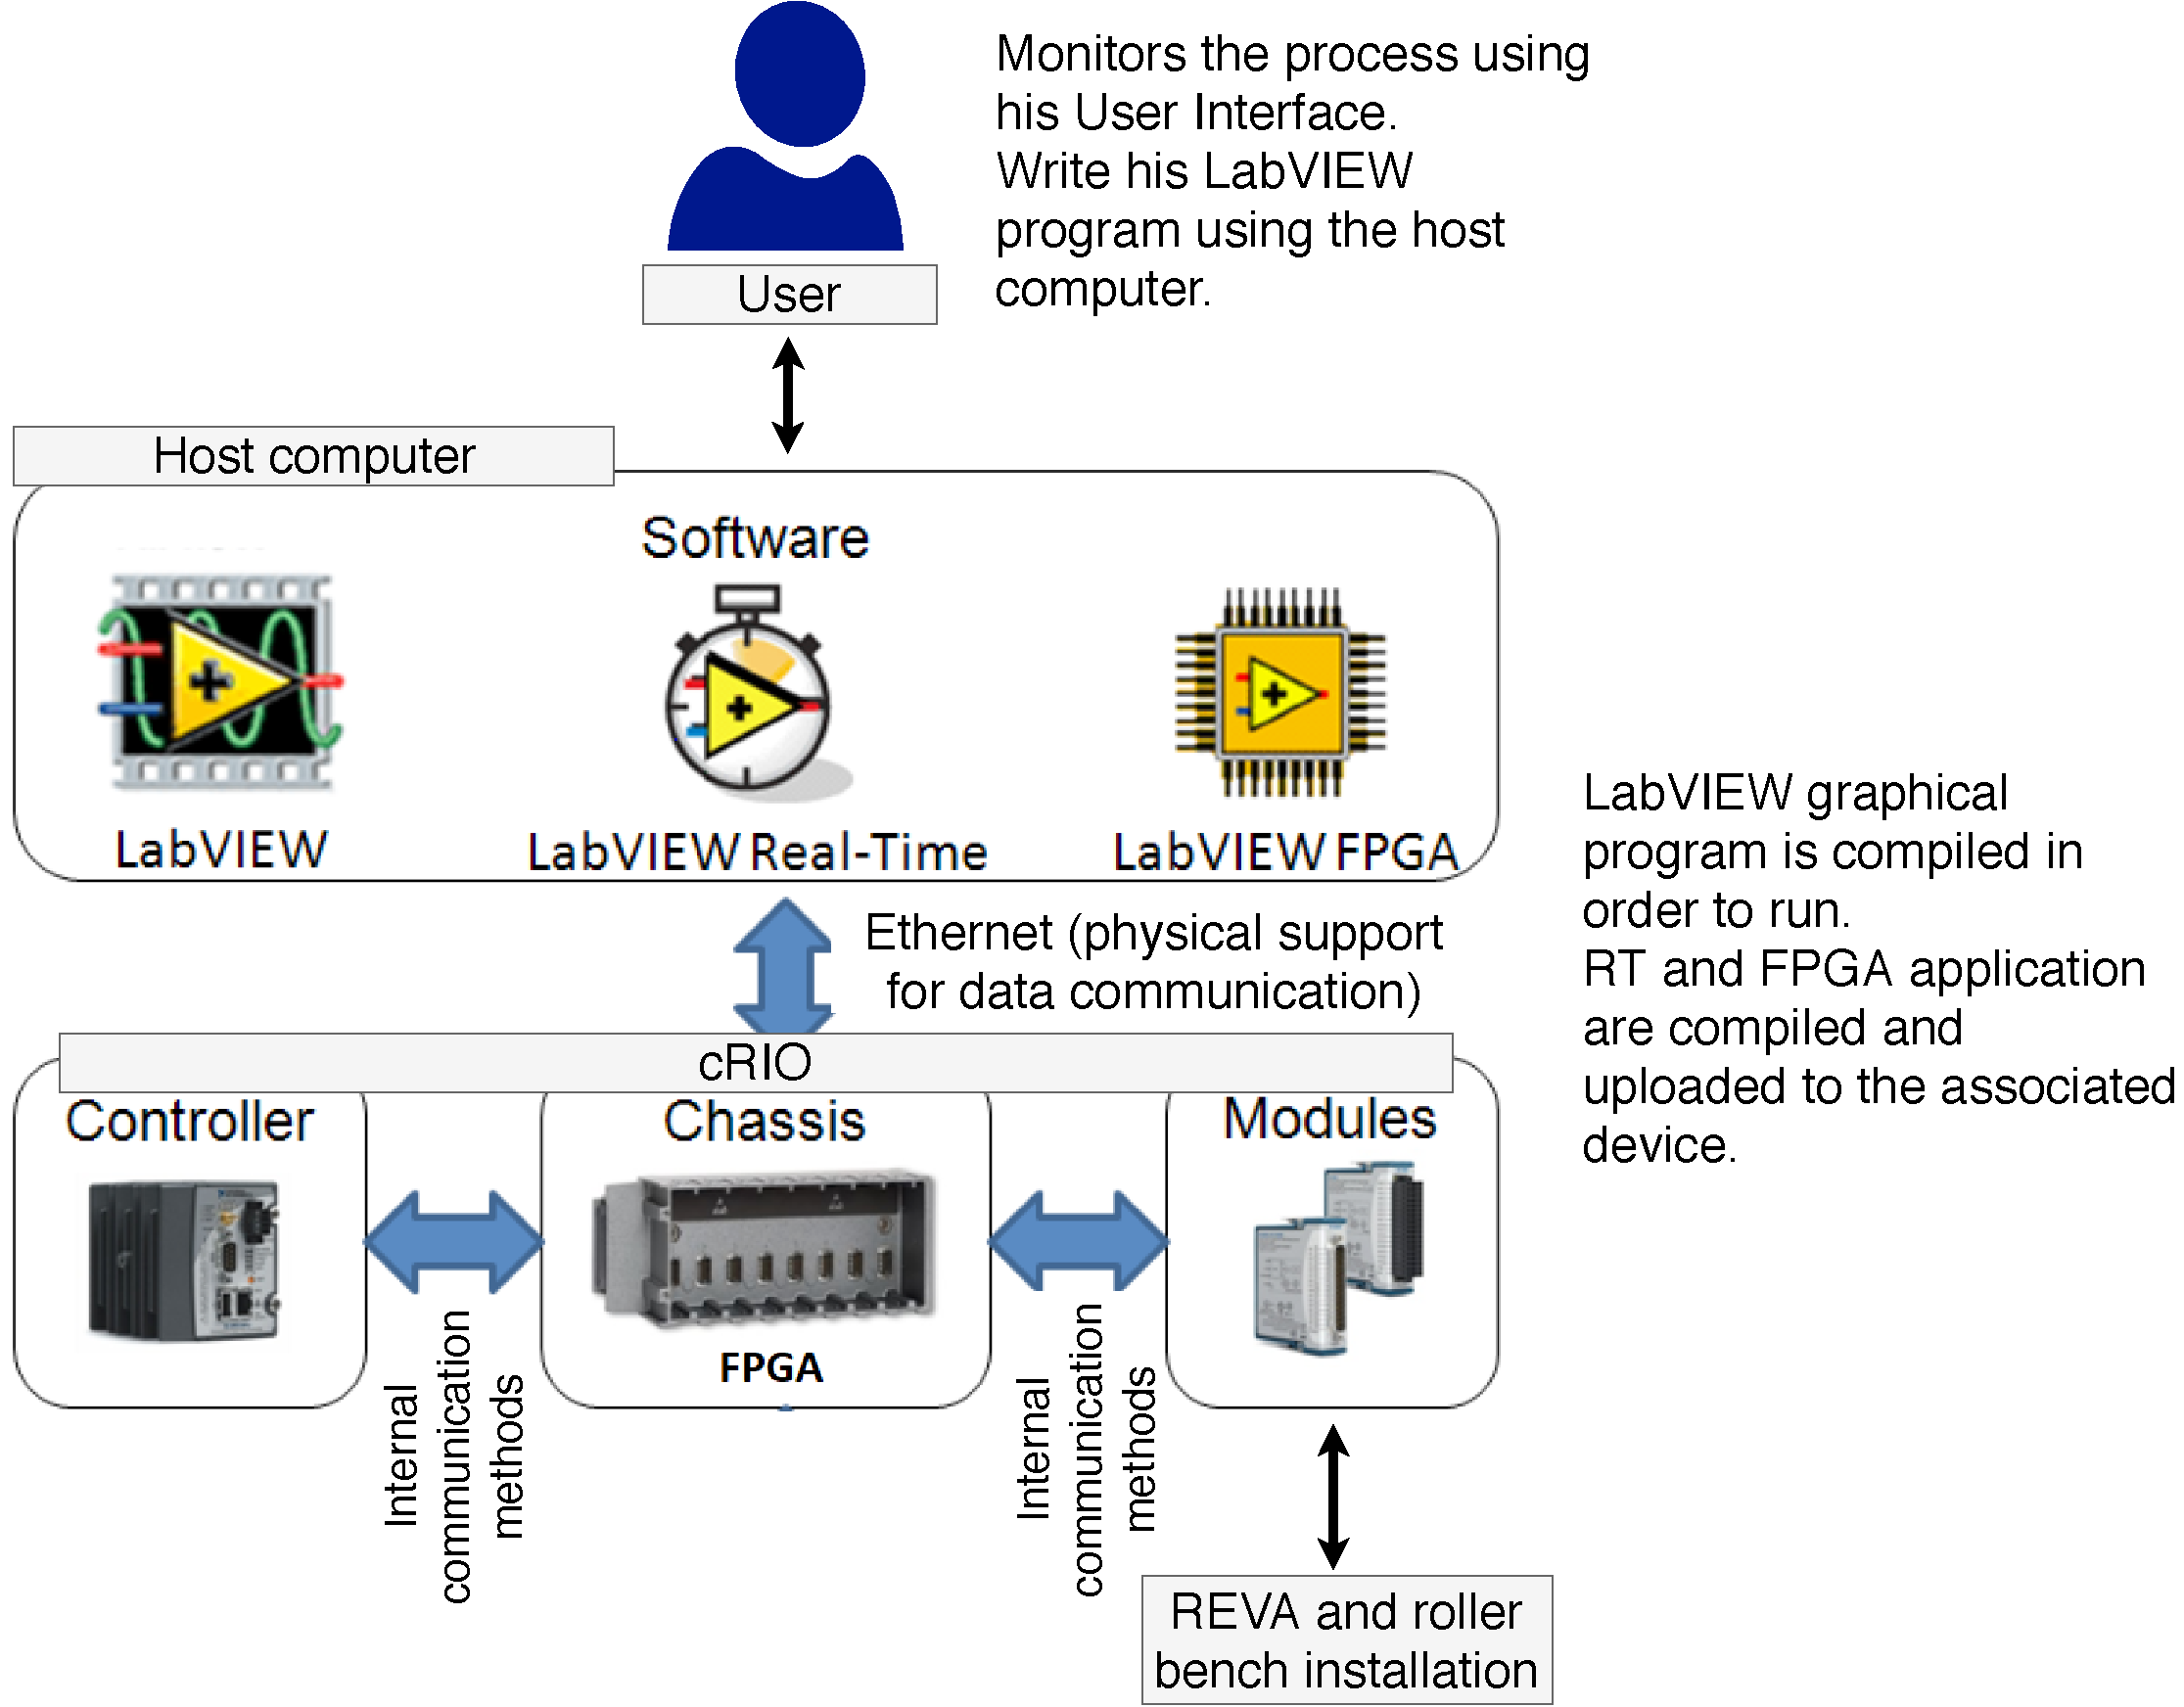
\includegraphics[scale=0.35]{figure/cRIO.pdf}
\caption{Components of a Complete cRIO System}
\label{fig:cRIOPrinicple}
\end{figure}
		\subsection{Development}
The practical choices in favor of LabVIEW and an attached \acs{crio} have been highlighted. Both of them were used in addition of the roller bench to develop a software and hardware combination capable of :
\begin{itemize}
\item[--] building the control loop based on \textsc{figure}~\ref{fig:GainSchedulingLoop}\footnote{However, in the final state of the project, the gain scheduling was not implemented} (p.~\pageref{fig:GainSchedulingLoop}).  
\item[--] feeding and designing a step signal to excite the REVA system in order to generate the datasets for identification procedures. 
\item[--] collecting the data measurements which will be later processed in DIAdem and used in MATLAB. 
\item[--] graphically controlling and monitoring the process
\end{itemize}

The practical implementation of the developed tool is illustrated in \textsc{figure}~\ref{fig:ToolSchem}. It clearly follows the typical feedback control system architecture. Moreover, it provides a clear distinction between the 4 participants involved; the LabVIEW environment, the \acs{crio} \acs{fpga} with its \acs{io} modules, the REVA system and the roller bench tool. 

The LabVIEW environment on the host computer ensures both an automatic and manual mode. The first one, is used when a \acs{pi} controller is wanted to control the system speed. The second manual mode is meant for general open-loop control and to achieve the system identification since it allows feeding a direct voltage signal (such as a step) to the REVA. Moreover, this environment computes the error between the speed reference and the actual vehicle velocity which is provided to the controller. The \acs{pi} parameters can be modified for on-line testing. It also provides a saturation function on the direct chain to limit the manipulated value voltage between 0~to~5~V\footnote{The Curtis 1236 input voltage limits}. Lastly, the data communication between the host and its \acs{crio} is ensured. Further explanation on the written program is provided in the subsection below. 

The hardware comprises the \acs{crio} \acs{fpga} input/output modules which ensures both data acquisition and conversion from a logical value into a physical voltage (and vice-versa). Additionally, an \acf{opamp} is introduced in the loop for signal conditioning purpose. Both \acs{fpga} program and \acs{opamp} installation are explained in the subsections below. 
\begin{figure}[hbtp]
\centering
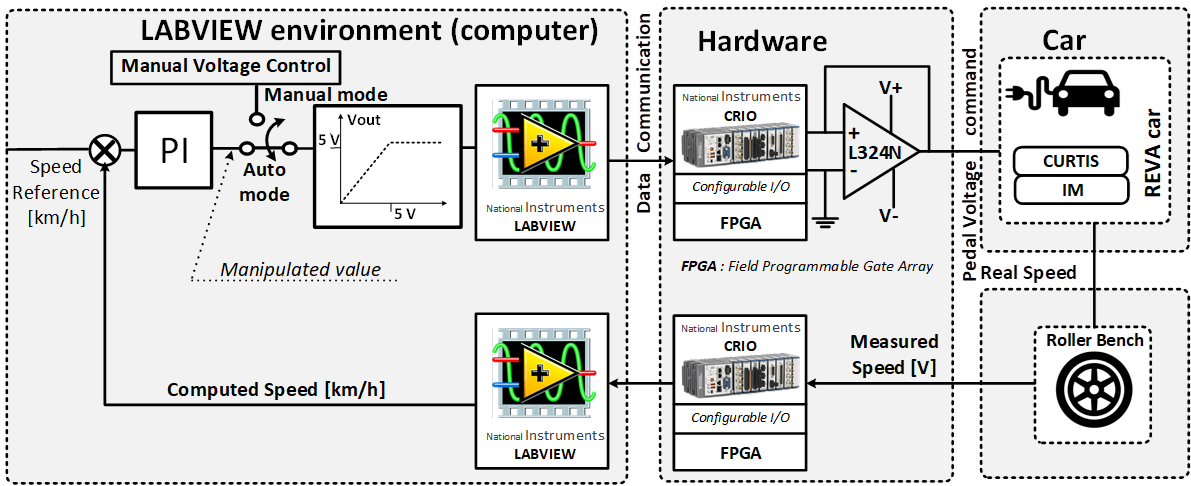
\includegraphics[scale=0.35]{figure/ProcessScheme.png}
\caption{Practical implementation of the developed tool}
\label{fig:ToolSchem}
\end{figure}

Finally, the REVA system receives the manipulated value that simulates its pedal voltage. The vehicle reacts to this input by generating a torque and rotational speed at its wheels which in return rotates the roller bench. Its embedded tachometer sent a speed measurement to the \acs{crio} which, in return, fed it to the LabVIEW (therfore, ensuring the feedback). Also, the roller bench ensures controlling the resistive torque perturbation applied to the REVA. 

			\subsubsection{Host computer LabVIEW program}
The host computer runs the LabVIEW main program which implements: 
\begin{itemize}
\item[--] the error calculation
\item[--] the \acs{pid} controller
\item[--] a command voltage threshold (0 to 5~V)
\item[--] the data recording for the system identification within a \acs{ni} .tdms file. Such file format is well integrated in LabVIEW and is generally used for high frequency recording. 
\end{itemize}

The main program is provided with a user interface shown in \textsc{Figure}~\ref{fig:UI} (p.\pageref{fig:UI}) which allows the user to monitor and interact with the program. \textsc{Figure}~\ref{fig:MainCode}~(p.\pageref{fig:MainCode}) and ~\ref{fig:MainCode_2} (p.\pageref{fig:MainCode_2}) illustrate the main program. It includes a main deterministic loop which iterates at a constant frequency. The loop is connected to the \acs{crio} FPGA target which allows to communicate with the targeted \acs{crio} at each iteration. Also, using this time loop was mandatory to ensures the temporal consistency while recording the data into a .tdms file. 

\begin{sidewaysfigure}[hbtp]
\centering
\includegraphics[width=\linewidth]{figure/Main_Program_1.png}
\caption{Host computer LabVIEW Program (1)}
\label{fig:MainCode}
\end{sidewaysfigure}

\begin{figure}[hbtp]
\centering
\includegraphics[scale=0.7]{figure/Main_Program_2.png}
\caption{Host computer LabVIEW Program (2)}
\label{fig:MainCode_2}
\end{figure}

\begin{figure}[hbtp]
\centering
\includegraphics[width=\linewidth]{figure/UI.png}
\caption{LabVIEW user interface}
\label{fig:UI}
\end{figure}

			\subsubsection{FPGA chassis design}
The \acs{crio} mainly ensures the communication between the LabVIEW environment and the process to be controlled and identified. Therefore, it must read the response and send the exciting command to the REVA. 

A \acs{fpga} is a reconfigurable electronic circuit; it contains multiple modular digital circuits that can be rewired together at wish. By selecting how each digital circuit are connected, the \acs{fpga} modifies its inputs differently, thus, a \acs{fpga} can be used to build almost any digital circuit. Such device is not a logical program but a real hardware with combinational and sequential circuits, and a signal is treated online by this physical hardware which reduce the processing time. Due to the infinite amount of possibilities and the fast signal treatment, \acs{fpga} devices are becoming more and more used. That being said, the \acs{crio} chassis is a \acs{fpga} which internal circuit can be rewired using LabVIEW. The graphical program is complied in low level language which designs the chassis internal connections. Since the input and output \acs{crio} modules are directly attached to the chassis, those signals can be acquired using the \acs{crio} FPGA. 

The graphical LabVIEW \acs{fpga} program is illustrated in \textsc{figure}~\ref{fig:FPGAProgram} (p.~\pageref{fig:FPGAProgram}). A 2-stage \texttt{sequence structure} is used. The first stage initializes the input and output modules from which the chassis must read or write the signals, and the settings information later required by functions in the code. The second stage contains a \texttt{while loop}, which allows the \acs{crio} to continuously acquire and provide the signals.  At each loop iteration, if the button is released (False), the main code within the \texttt{conditional structure} is executed. The \texttt{Control pedal voltage} variable is directly linked to its associated module (Mod3/AO3), and therefore, the physical output of the module follows the value of its linked variable. The rotational speed measurement of the roller bench is acquired using the same technique; the physical signal can be acquired from Mod1/AI1. This tachometer measure provides an AC signal which must to be converted into a constant speed value, reason why its \acs{rms} value is computed by the appropriate \acs{rms} block. The linear interpolation aim is to smooth the computed \acs{rms} value of the roller speed into a regular speed distribution. Finally, the \acs{rms} interpolated  value of the roller speed is then converted from radiant per second into the linear velocity of the vehicle in kilometer per second. Besides, an offset correction is applied to the measure avoiding having residual speed measure at low speed. 
\begin{sidewaysfigure}[hbtp]
\centering
\includegraphics[scale=0.65]{figure/FPGA-meas.png}
\caption{LabVIEW FPGA program. Output writing and input speed from sine to \acs{rms} conversion}
\label{fig:FPGAProgram}
\end{sidewaysfigure}

		\subsubsection{Hardware development}
The \acs{crio} NI 9263 is an analog output module voltage which converts the logical signal generated from LabVIEW into a physical voltage provided to the system. Even if its 0 to 10~V operating range complies with this application (0 to 5 V required), its maximum output current is limited to 1 mA. This maximum current value limits the available power that can be supplied to the REVA. In practice, it appeared to be lower than the minimum power required to excite the motor drive instead of the gas pedal. The vehicle auxiliary power supply that powers the pedal potentiometer is indeed rated at maximum of 200~mA, 200 times higher than the current provided by the NI 9263. Buying another module was too expensive and no other one was available, therefore an Operational Amplifier has been used to solved this problem. 

\begin{figure}[H]
\centering
\includegraphics[scale=0.3]{figure/noneinvertingOpAamp.png}
\caption{Op Amp in voltage following configuration~\cite{platt2014encyclopedia}}
\label{fig:NonInvOpAmp}
\end{figure}

An Op Amp is made of multiple transistors packed in an integrated circuit chip. It senses the voltage difference between 2 inputs and uses an external power supply to amplify the signal. It uses a negtive feedback to ensure the output signal closely replicates the input. The amplification ratio is adjusted using external resistances~\cite{platt2014encyclopedia}. Since the Op Amp uses an external power supply, the available power supplying the output circuit increases (depending on the Op Amp characteristics). In this particular case, the available current must be increased while the Op Amp output voltage must follow the NI 9263 signal. Such problematic is solved by using a common voltage follower circuit shown in \textsc{figure}~\ref{fig:NonInvOpAmp} where the Op Amp output is connected to its non-inverting input. 

In practice, the \acs{vub} possess many cheap LM324N Op Amps that can provide an output current of 50 mA. It has been practically proven to supply the motor drive put ineffectively while used in a voltage follower configuration. The major drawback of Op Amp is the slew rate and their output attenuation at high frequency. In this use case, both of those effects would not influence the output voltage nor the process, since the voltage frequency remains low and the slew rate is not critical in this application. 

	\section{Illustrated procedure and result}
The theoretical approach for identifying the REVA system and a PI controller have been proposed. The tools for achieving the identification have been implemented and the control loop has been built. The following section illustrates the procedure for finding the \acs{pi} parameters and provides its associated regulated system response. 

\begin{itemize}
\item[--] Using the proposed LabVIEW user interface, an input throttle voltage is fed to the REVA until the desired operating point is reached. Then an excitation step of the desired amplitude is applied and the process is left until it reaches a steady state speed. (\textsc{figure}~\ref{fig:Process_example})
\item[--] The LabVIEW program will generated a .tdms measurement file at the end of the experiment. Using DIAdem, the data can be visually inspected and filtered (\textsc{figure}~\ref{fig:Filtering}) and the file must be converted from tdms into xls format. Once, this measurement is imported in MATLAB, the offsets and trends of the input and output measurements are removed and usable data range where a linear system is select (\textsc{figure}~\ref{fig:ExperimentSelect}) 
\item[--] The system identification toolbox allows to estimate the model parameters (first order model in this case study)(\textsc{figure}~\ref{fig:MTALABSysID}) . The experimental data and the estimated model must be compared to validate the experiment. (\textsc{figure}~\ref{fig:data_estimated_response}) 
\item[--] Using MATLAB PID tuner and the generated model, the PI parameters can be estimated (\textsc{figure}~\ref{fig:PI_param_iden}) 
\item[--] Using the User Interface, the PI can be configured to regulate the vehicle speed around the selected operating point. (\textsc{figure}~\ref{fig:Example_speed_reg}) 
\end{itemize}

\begin{figure}[hbtp]
\centering
\includegraphics[width=\linewidth]{figure/Example_process.eps}
\caption{Example process for system identification}
\label{fig:Process_example}
\end{figure}

\begin{figure}[hbtp]
\centering
\includegraphics[width=\linewidth]{figure/Speed_Filtered.eps}
\caption{Speed measurement filtering}
\label{fig:Filtering}
\end{figure}
			
\begin{figure}[hbtp]
\centering
\includegraphics[width=\linewidth]{figure/Experimental_data_collected.eps}
\caption{Usable measurement for system identification}
\label{fig:ExperimentSelect}
\end{figure}

\begin{figure}[hbtp]
\centering
\includegraphics[width=\linewidth]{figure/using_matab.png}
\caption{MATLAB System identification toolbox (example)}
\label{fig:MTALABSysID}
\end{figure}
	
\begin{figure}[hbtp]
\centering
\includegraphics[width=\linewidth]{figure/data_estimated_response.eps}
\caption{Experimental data and estimated model comparison}
\label{fig:data_estimated_response}
\end{figure}
	
\begin{figure}[hbtp]
\centering
\includegraphics[width=\linewidth]{figure/PID_tuner.png}
\caption{PI controller identification within MATLAB $k_p = 0,39715$ and $k_i=1,2259$ (or $I = k_i^{-1}=0,82$)}
\label{fig:PI_param_iden}
\end{figure}
	
\begin{figure}[hbtp]
\centering
\includegraphics[width=\linewidth]{figure/test_low_speed.jpg}
\caption{Successful example of REVA speed regulation between 5 and 10~km/h using the system identification method}
\label{fig:Example_speed_reg}
\end{figure}

\begin{figure}[hbtp]
\centering
\includegraphics[width=\linewidth]{figure/PID_output_2.eps}
\caption{Typical speed regulation example (set point 10~km/h) using system identification}
\label{fig:PID_TOR}
\end{figure}

\textsc{figure}~\ref{fig:Example_speed_reg}\footnote{There is an error in the user interface, the reference (SP) is the red curve while the blue curve is the REVA speed} illustrates the regulation achieved by the PI controller which parameters have been identified using the illustrated method provided above. The actual speed of the REVA (in blue) follows the chosen set point between 5 and 10~km/h (in red) as excepted. Oppositely, \textsc{figure}~\ref{fig:PID_TOR} illustrates a more typical result of the identification process where the \acs{pi} controller is inappropriate and could not regulate the REVA speed.


The system identification inertly depends on the quality of the dataset provided to the toolbox and the pre-processing must be undertaken carefully. Additionally, to ensure the tracking of a speed profile as originally proposed, the identification process must be repeated several times for multiple operating points. The identification itself is also an iterative process, and when a data is not valid another set must be measured once the problem is solved. However, in this case study, the problem comes form the system  state itself; the REVA couldn't provide enough time in steady state condition to allow the identification. Therefore, as highlighted by \textsc{figure}~\ref{fig:Citical_loop} the identification process is forced into a critical loop. 

\begin{figure}[hbtp]
\centering
\includegraphics[scale=0.8]{figure/Critical_loop.pdf}
\caption{System and controller identification critical loop}
\label{fig:Citical_loop}
\end{figure}


	\section{Experiment issue}\label{sec:experiment_issue}
		\subsection{Situation assessment}
While testing the parameters deduced from the identification process a problem with the REVA arisen. During this experimentation, the resitive torque was kept constant and minimal. First, the system was brought near the operating point of 21~km/h for which the \acs{pi} paramaters have been evaluated according the previously described procedure. The expected response (in the best situation) should be converging into a steady-state close to the operating point. The \acs{pi} regulated REVA provided the response illustrated in \textsc{figure}~\ref{fig_PID_tuning}; once in automatic mode, the PI regulates the REVA as bang-bang controller. Instead of converging to a steady value, the controller acts as a bang-bang controller which oscillates between the threshold values. Therefore, the REVA speed does not reach a steady value neither. Obviously, the PI parameters are not adequate. 

While tuning the controller parameters to reduce the steady state oscillation, the car had suddenly stopped working. The regulation loop has has switched into manual mode and a 0~V gas pedal had been set and the mechanical switch had been opened. 

\begin{figure}[hbtp]
\centering
\includegraphics[width=\linewidth]{figure/PID_tuning_2.jpg}
\caption{REVA speed regulation (above) and PI command (below) (set point: 21~km/h PI parameters: $K_p = 3,5$ $I=1,8$)}
\label{fig_PID_tuning}
\end{figure}

		\subsection{Issue: damaged battery}
Once the REVA had been secured, visual statements, continuity tests and voltage measurements have been undertaken to verify the REVA condition. Those statements results are provided in \textsc{table}~\ref{tab:Statement_result}. 

The REVA mechanical and electrical components are not damaged. However, the battery voltage measurements does not comply with the expected values (13,3~V for across a single battery and around 40~V across all of the them). The battery pack has been dismantled and each battery voltage has been measured separately; the battery on the left provided 1,55~V while the two others provided a normal value of 13,3~V. As a result, the unexpected measurements across the batteries were caused by this single damaged power source. This battery model is equipped with both a fuse and an internal protective circuit. Even if the damaged battery fuse was intact, it can be seen that it has already been changed, which lets believe this particular battery had been already damaged in the past. While testing and tuning the \acs{pi} controller, the highly varying command generated induced large current gradients flowing from the batteries to the REVA. Most likely, the damaged battery was already more sensitive and reacted to those gradients by activating its protection circuit. The measurement in \textsc{figure}~\ref{fig:BatVoltMeasSwitchClosed} provides such a low voltage, since the internal protective circuit was opened. This battery has been removed and the fourth available one has been used instead. 

\begin{figure}[hbtp]
\centering
    \includegraphics[scale=0.6]{figure/Batteries_measure.png}
    \caption{Battery voltage measurements (top view of the setup)}
    \label{fig:BatVoltMeasSwitchClosed}
\end{figure}

% Please add the following required packages to your document preamble:
% \usepackage[normalem]{ulem}
% \useunder{\uline}{\ul}{}
\begin{table}[H]
\centering
\begin{tabular}{|l|l|}
\hline
\multicolumn{1}{|c|}{{\ul \textbf{Statement}}} & \multicolumn{1}{c|}{{\ul \textbf{Result}}} \\ \hline
\multicolumn{2}{|c|}{\textbf{Visual  statement}}                                            \\ \hline
Mechanical issues                              & No                                         \\ \hline
Electrical connections                         & Well pluged, undamaged                     \\ \hline
\multicolumn{2}{|c|}{\textbf{Continuity test}}                                              \\ \hline
Relay                                          & No short-circuit                           \\ \hline
Mechanical switch                              & No short-circuit                           \\ \hline
Motor                                          & No short-circuit                           \\ \hline
Fuses                                          & Functional                                 \\ \hline
Curtis                                         & No short-circuit                           \\ \hline
\multicolumn{2}{|c|}{\textbf{Battery voltage measure}}                                      \\ \hline
\multicolumn{2}{|c|}{\textit{Battery pack in open circuit}}                                 \\ \hline
Across battery (left) (\textsc{figure}~\ref{fig:BatVoltMeasSwitchClosed})                          & 1,5 V                                      \\ \hline
Across battery pack    (\textsc{figure}~\ref{fig:BatVoltMeasSwitchClosed})                        & 39,86 V                                    \\ \hline
\multicolumn{2}{|c|}{\textit{Battery pack  in close circuit}}                               \\ \hline
Across battery (left) (\textsc{figure}~\ref{fig:BatVoltMeasSwitchClosed})                         & 26,5 V                                     \\ \hline
Across battery (left and center) (\textsc{figure}~\ref{fig:BatVoltMeasSwitchClosed})                & 13,25 V                                    \\ \hline
Across battery pack (\textsc{figure}~\ref{fig:BatVoltMeasSwitchClosed})                           & 0,048 V                                    \\ \hline
\end{tabular}
\caption{REVA statement results for diagnostic}
\label{tab:Statement_result}
\end{table}

\section{Summary and conclusion}
The objective of this chapter is to develop a speed control automated feature for the REVA prototyping platform. This case study focuses on the throttle pedal actuation and the braking has not been integrated. The speed controller development involved 3 phases; (1) the theoretical approach investigation and selection, (2) the control loop implementation, the required tools building or selection and (3) the theoretical approach application. 

The REVA speed control close-loop for achieving the tracking has been built. Its principle relies on the natural way a driver regulates the motor torque using the throttle pedal to follow his desired speed. The developed controller provides a command to the REVA system to regulate the torque requests instead of the driver. The REVA system was divided into 3 sub-subsystems: (1) the Curtis 1236 (motor drive in torque mode), (2) the induction motor and (3) the vehicle dynamic. Next, using the open-loop system responses to steps excitation, the operating region where the controller development is achievable was identified between 0 to 35~km/h and the REVA open-loop characteristic was plotted. 

The approach to build a mathematical model of the REVA speed dynamic to identify the controller parameter was chosen.  The first principle modeling relies on the system equations to build an appropriate model while the system identification relies on experimental data to identify the parameters of a chosen model. Because of the unknown algorithms of the Curtis 1236, the first principle modeling was stated as not achievable, and the system identification process has been selected. Knowing a self generated throttle input signal and measuring the REVA speed output, the system identification provides the model parameters. At this stage, the REVA system has been simplified; because of material issues the vehicle dynamic sub-system has been omitted and replaced by a torque perturbation at the REVA's wheels. For its simplicity, linear first order models were used to approximate the REVA dynamic. Since its dynamic is non-linear, multiple linear models were required to describe this dynamic at each speed. Next, multiple controller types have been studied and the \acs{pi} + gain scheduling has been selected because of its simplicity and its implementation easiness. The gain scheduling stores multiple \acs{pi} parameter sets, and, depending on the REVA speed, provides the adequate PI parameters to the PI controller enabling the speed control between 0 to 35~km/h. 

Next, using LabVIEW on a host computer and an attached \acf{crio}, both the speed control loop and the tools for achieving the system identification have been realized. The \acs{fpga} chassis of the \acs{crio} receives and converts the roller bench speed measurements. The host computer implements the \acs{pi} controller which computes the command signal sent to the REVA through the \acs{fpga} chassis and an operational amplifier used to increase the signal current. Additionally, the host computer was used to generate the step input signals and to record the REVA speed response for the system identification. The implemented user interface was used on the host computer to monitor and control the REVA speed (manually and automatically). 

The experimental data for the system identification was recorded using the self-made tools. Using DIAdem software, the data is visually inspected and filtered. Next, using MATLAB, the data offsets and trends are removed, and the usable data is selected. Then, using system identification toolbox and the processed data, the first order model is computed. Using the MATLAB PID tuner, the PI parameters are deduced and tested on the implemented speed control loop. Then the process must be repeated to fill PI gain scheduling table. 

Even if the proposed method has practically proven to provide a single successful model and its related \acs{pi} controller, most of the identification processes had failed. Indeed, the system identification is very sensible to the quality of the experimental data. The REVA switch into a safety mode reducing the wheel torque adding trends in the data. Moreover, the working time of the vehicle is too short to provide sufficiently large datasets. Therefore, in order to accomplish the system identification it is mandatory the improve the REVA state. The REVA first order models were not approximated due to the lack of reliable data, and neither were the associated PI parameters. Therefore, speed controller couldn't be fully completed.  


%\chapter{Computer vision : software development \label{chap:computer_vision}}
As stated in chapter~\ref{chap:StateOfArt}, highly automated vehicle's key achievment is software development. In this chapter, a special focus on the environment and perception modeling is addressed. More specifically, this chapter delves few computer vision techniques used to achieved \textit{lane detection}, \textit{traffic sign classification}, \textit{vehicle detection and classification}, and \textit{behavioral cloning}. Each of those perception task is realized using one of the popular and simple programming language; Python. 

This chapter is a personal summary of my enrollment in the Udacity Self Driving Cars nanodegree~\cite{Udacity} which I completed in parallel of this master thesis. Each computer vision technique problematic solution described here are my personal project course achievements. Even if the proposed code must be optimized, they have proven to work and might be useful to the \acs{vub} while building an autonomous REVA. 
	\section{Lane detection}
	\section{Traffic sign classifier}
	\section{Vehicle detection}
	\section{Behavioral cloning}
In this case, behavioral cloning is the art of teaching a machine to act similarly to a human. \acf{cnn}, is a particular structure of \acf{nn} which have proven to be powerful at pattern recognition from images, and their usage have increased in environment perception. This project aim is to apply this deep learning technique to mimic the human driving behavior; using images from dashboard cameras, the \acs{cnn} is trained to predict the steering angle to be applied to the vehicle. This method have been successfully been applied on the real road condition by Nvidia~\cite{NvidiaBC}. Even such complex \acs{nn} requires carefulness about the training process, this method skips the environment perception problem decomposition which decrease the complexity of achieving automated vehicle. However, as general statement while using \acs{nn}, the prediction process acts as a black-box and it is merely impossible to access what is happening inside it, and therefore knowing the used feature to make the prediction. Knowing this, it this development level, the decomposition of environment prediction is preferred since it allows scoring the efficiency of the each sub-tasks which is impossible while applying \acs{cnn}. 

For ease, Udacity provides a video-game like simulator which permits one to drive a vehicle around two virtual tracks while recording the steering angle and captures images from the dashboards cameras. It eases the process of data collection and validation, which would have been more complicated using a real vehicle on real road. Two tracks are available in the simulator, a simple one used to collect the data and validate the \acs{cnn} architecture, and secondly, a more challenging to validate network prediction generalizes well and extracts meaningful features. 

Hence, the project objective is to develop a \acs{cnn} structure, which will be trained to correlates the dashboard images (vehicle state) to a steering angle. Using a \acs{pi} controller within the simulator and the car will move at a constant speed as a driver would regulate the speed. 

The project can be decomposed in the following steps:
\begin{itemize}
\item[-] Use the simulator to collect data of good driving behavior 
\item[-] Build a pipeline that preprocess the gathered data
\item[-] Build, a convolution neural network in Keras which is capable to predicts steering angles from images 
\item[-] Train and validate the model with a training and validation set 
\item[-] Test that the model successfully drives around track one without leaving the road 
\end{itemize}
		\subsection{Data}
			\subsubsection{Data collection}
The dataset is generated while manually driving the car on the test
track of the simulator. The software captures images from 3 different
dashcameras, a center, left and right one as well as the steering angle once the recording button is pressed. All these measurements are saved in a specified directory and the file path of the images is related to the measured steering angle in a .csv file. 

The procedure to collect the data consists of two steps : 
\begin{itemize}
\item[-] Driving the car smoothly for 3 laps clockwise and 3 laps counter clockwise. These data will teach the \acs{nn} to drive in the center part of the road. 
\item[-] Perform recovery center driving for 2 laps clockwise and counter clockwise. This
consists of getting closer to the lateral extremities of the track (while not recording) and then get back to the center lane while recording the measurement. Without the second step of data collection, in autonomous driving, the car is not trained to deal with critical situation where it gets closer and closer of a border lane. Instead of getting back on the center lane, it just steers normally and, worst case, get off the track.
\end{itemize}

The dataset is then loaded into a panda\footnote{Indeed, Panda is a powerful python library based on C programming language which is build to treat large amount of data. It has become popular while dealing with \acs{nn} which requires large datasets.} DataFrame in python which fits the need of fast data processing. This procedure provided a dataset of
37000 raw samples. Moreover, I've tried to have the same amount of data for each case, thus
when balancing the data each state of the car (recovery or driving in
center) has the same probability to be fed into the Neural Network.
Thinking of it, it might be more interesting to have more center driving
data since it is the normal behavior of driving ; this way the wiggling
I face may be limited.
%\chapter{Future work \label{chap:future_work}}
\section{First things first}
The REVA is a great vehicle for student willing to investigate electric vehicle. 
\section{Towards an embedded system}
\section{Software improvement}

\chapter{Conclusion}\label{sec:conclusion}
This master thesis purpose was to investigate how to transform the VUB's REVA electric  vehicle into an autonomous vehicle. The work has been tackled in 3 phases discussed below. 

The autonomous vehicles field has been investigated and the general framework of such vehicles has been provided. This framework ensures the environment perception, the localization, the mapping, the decision making, the path planning and finally the motion control. Those tasks rely on multiple algorithms requiring high computational power. Having an electric vehicle prototype that is already mechanically and electrically designed, the main transformation work stays in the embedded software and hardware development. Having limited knowledge in programming and larger skills in control engineering, this master thesis focused on the motion control, especially the speed tracking. 

The REVA electric platform was brought in the VUB's laboratory and its current state has been assessed. Prior to this thesis, the original REVA batteries were stated inoperable and were removed. After acquiring the vehicle, another battery pack has been plugged and the REVA driving behavior has been analyzed. According to the measurement results, the driving performances were abnormal. The diagnostic stated that the motor drive and the \acf{ems} were not calibrated with regards to the new batteries voltage, resulting in (1) a limited driving torque and (2) the random occurrence of a safety procedure that reduces the REVA speed until it stops. The possibility to re-calibrate the electronic components according the new batteries was investigated, and concluded the \acs{ems} and the motor drive were proprietary devices with unaccessible and unmodifiable parameter access. 

The REVA speed controller has been investigated but has shown to be unachieveable. The chosen control strategy simulates the human actuation of the throttle hence replacing the human torque requests provided to the REVA. The system identification technique has been chosen to build multiple linear mathematical models of the vehicle and a PI + gain scheduling controller has been chosen. Using the VUB roller bench, LabVIEW programming on host computer and an attached \acs{crio}, the associated control loop has been implemented as well as the data recording tools for achieving the system identification. Because of the REVA nonoperational state, the recordings were unreliable and disrupted the data-driven modeling. Hence, the models were not estimated neither were the PI parameters. For this, reason the speed controller couldn't be fully completed. 

Initially, the project started with the assumption that the current REVA vehicle could be used to investigate the transformation from an electric vehicle to an autonomous vehicle. After a more in-depth analysis, we can conclude the REVA is not yet in an optimal starting point. The REVA has operational issues caused by the new battery set and lacks of available components knowledge for achieving such a transformation. The \acs{ems} and the motor drive are the components that are obstructing the transformation. Replacing those by self-made devices would provide a better knowledge of the vehicle enabling using the actual batteries. Moreover, it would provide a drive-train mathematical model allowing simulating the REVA dynamic. Additionally, to achieve the full transformation of the REVA from an electric to an autonomous stage, it would be worth to divide the whole project into multiple smaller projects by specific domain. 

\cleardoublepage
\printbibliography[heading=bibnumbered,
title={Bibliography}]

\cleardoublepage
\appendix
\chapter{Curtis 1236 data}
	\section{Basic wiring diagram}
\begin{figure}[hbtp]
\centering
\includegraphics[scale=0.65]{figure/Curtis1236_wiring_diagram.png}
\caption{Basic wiring diagram of Curtis 1236 motor controller~\cite{Curtis_User_Manual}}
\end{figure}
	\section{REVA Curtis Parameters}\label{s:REVACurtisParam}
\includepdf[pages=-,pagecommand={\thispagestyle{plain}},]{code/REVAL-ionParameterListOS.pdf}


\chapter{Data processing VB script}\label{anexe:VBscript}
\begin{footnotesize}
\lstinputlisting[language=VBscript, breaklines=true]{code/Full_v2.VBS}
\end{footnotesize}

\chapter{Using the didicated cRIO for data acquisition}\label{sec:cRIOdataAcq}
\section{Procedure}
\label{anc:cRIO}

Compact redefinable input and output (cRIO) enables measuring multiple values synchronously at defined rate. This measurement tool is practical but inconvenient to use on old XP-laptop provided by the VUB. 

Since students show difficulties to connect their laptop to the cRIO, this section provides a fast procedure to communicate with it. 

One must understand that the cRIO is configured as a server, thus it is possible to access the device on local network through an Ethernet cable. 
\subsection{Software}
The LabVIEW Run Time 2010 must be installed on the user computer who is willing to communicate with the cRIO. It can be downloaded on the National Instrument website. 
\subsection{IP config}
One should make sure his computer is on the same network as the device. Open your command prompt (cmd) and execute the \texttt{ipconfig} command to verify the computer IP address and subnet mask. If your subnet is not \texttt{255.255.255.0} else change your computer network parameters in the computer settings.  

\subsection{File access}
You can collect the data from the cRIO using FTP protocol. Open, your file browser, paste the following path \texttt{\url{ftp://169.264.125.17/}}, and you will have access to the device registered data.

\subsection{Panel access}
A friendly Control Panel has been implemented within the cRIO to easily interact with the user. You can access it using HTTP protocol through the 8000 open-port of the device. Open Internet Explorer web browser, paste the following path \url{http://169.254.125.17:8000/vi/cRIO\_Main.html} to access the panel. Due to compatibility issue, it is not possible to access the panel with another browser, therefore MAC user will ne be able to use the cRIO.

\subsection{Procedure}
The procedure to collect the data using the front panel : 
\begin{enumerate}
\item Activate \textit{STOP waiting} button. 
\item Select a \textit{off.cfg}, click on \textit{preview} button than \textit{apply} button. User must be gentle while using the cRIO front panel because of the device latency. 
\item Configure your measurement process by activating and selecting the sampling rate than click\textit{apply} button. If your are using an existing configuration, select your \textit{cvg} file, click on \textit{preview} button than \textit{apply} button. 
\item Once the measures are done, select a \textit{off.cfg}, click on \textit{preview} button than \textit{apply} button. Collect your data via the FTP access of the cRIO. 
\end{enumerate}

\cleardoublepage
\end{document}
